\documentclass[12pt]{report}

%%
% to enumerate subsubsection
%%
\addtocounter{tocdepth}{3}
\setcounter{secnumdepth}{3}
% \usepackage{tgtermes}
\usepackage[a4paper, margin=1in]{geometry}
\usepackage[T1]{fontenc}
\usepackage[breaklinks,hidelinks]{hyperref}
\usepackage[utf8]{inputenc}
\usepackage{graphicx} 
\usepackage{tikz}
\usepackage{amsmath, amssymb}
% \usepackage{indentfirst}
% \usepackage{cite}
\usepackage{natbib}
\usepackage[nameinlink,noabbrev]{cleveref}
\usepackage[capposition=top]{floatrow}
\usepackage{float}
\usepackage{caption}
\usepackage{xfrac}
\usepackage{braket}
\usepackage[toc,page]{appendix}
\usepackage{tabularx}
\usepackage{adjustbox}
% \usepackage{hyperref}
% \usepackage{physics}

%%
% to enumerate subsubsection
%%
\addtocounter{tocdepth}{3}
\setcounter{secnumdepth}{3}

% Snippet
\newcommand{\BSM}{Black--Scholes--Merton }
\newcommand{\lnorm}{log-normally }
\newcommand{\bmotion}{Brownian Motion }
\newcommand{\stvar}{stochastic variable }
\newcommand{\wienpro}{Wiener process }
\newcommand{\markpro}{Markov process }

% 
% Bunch of new commands
% 
% brownian motion
\newcommand{\dBm}{dW\left(t\right)}
\newcommand{\dpoiss}{dq\left(t\right)}
\newcommand{\DBm}{\delta{W\left(t\right)}}
\newcommand{\Bm}{W\left(t\right)}
\newcommand{\Bmsub}[1]{W_{#1}\left(t\right)}
\newcommand{\Dt}{\Delta t} 
\newcommand{\Bmdist}{\DBm \sim N \left( 0, \Dt \right)}
\newcommand{\ft}{f\left(t, \Bm \right)}
\newcommand{\E}{\mathop{\mathbb{E}}}
\newcommand{\ct}{c\left(t, x\right)}
\newcommand{\dcx}{\frac{\delta\ct}{\delta x}}
\newcommand{\dciix}{\frac{\delta^2\ct}{\delta x^2}}
\newcommand{\dct}{\frac{\delta\ct}{\delta t}}
\newcommand{\N}[1]{N\left(#1\right)}
\newcommand{\dsub}[1]{d_{#1}\left(\Dt, x\right)}
\newcommand{\call}[2]{c\left( #1, #2\right)}
% % about stock
\newcommand{\St}{S\left(t\right)}
\newcommand{\Vt}{V\left(t\right)}
\newcommand{\Si}{S\left(0\right)}
\newcommand{\dSt}{dS\left(t\right)}
\newcommand{\DSt}{\Delta S\left(t\right)}
\newcommand{\dSr}{\frac{\dSt}{\St}}
\newcommand{\DSr}{\frac{\DSt}{\St}}
\newcommand{\Scontinuous}{\St = \Si e^{\sigma\Bm + \left(\alpha - \frac{1}{2 \sigma^2}\right)t}}
\newcommand{\Itobmdiff}{d\ft = \left[\frac{\partial \ft }{\partial t} + \frac{1}{2} \frac{\partial ^2\ft }{\partial x^2}\right]dt + \frac{\partial \ft}{\partial x} \dBm}
\newcommand{\Scontinousdiff}{d\St &= \alpha \St dt + \sigma \St \dBm}
\newcommand{\Scontinuousrate}{\dSr &= \alpha dt + \sigma \dBm}
 \newcommand{\Sdiscretediff}{d\St &= \alpha \St \Dt + \sigma \St \dBm}
\newcommand{\Sshort}{\Si e^{X}}
\newcommand{\CCRdist}{X \sim N\left(\left(\alpha - \frac{1}{2}\sigma^2\right)t, \sigma^2 t\right)}
\newcommand{\Sdiscreterate}{\DSr &= \alpha \Delta t + \sigma \DBm}
\newcommand{\Sdiscreterateexp}{\E \DSr = \alpha \Dt}
\newcommand{\Sdiscreteratevar}{var \DSr = \sigma ^2 \Dt}
\newcommand{\Sdiscreteratedist}{\DSr \sim N\left(\alpha\Dt, \sigma\Dt\right)}
\newcommand{\Sexp}{\E\St = \Si e^{\alpha t}}
\newcommand{\Svar}{var\St = \Si^2 e^{2\alpha t}\left(e^{\sigma^2 t} - 1\right)}
\newcommand{\Sshortt}{\St = \Si e^{X t}}
\newcommand{\CCRt}{X = \frac{1}{t} \ln{\frac{\St}{\Si}}}
\newcommand{\CCRtdist}{X \sim N\left(\alpha - \frac{\sigma^2}{2}, \frac{\sigma^2}{t}\right)}
\newcommand{\BSMpde}{\dct + r x \dcx + \frac{1}{2} \sigma^2 x^2 \dciix = r\ct}
\newcommand{\BSMeq}[1]{r\call{t}{#1} = \frac{\partial \call{t}{#1}}{\partial t} + r #1 \frac{\partial \call{t}{#1}}{\partial #1} + \frac{1}{2} \sigma ^2 #1 ^2 \frac{\partial ^2 \call{t}{#1}}{\partial #1 ^2}}
\newcommand{\BSMGreeks}[1]{r\call{t}{#1} = \Theta + r #1 \Delta + \frac{1}{2} \sigma ^2 #1 ^2 \Gamma}
\newcommand{\BSMsol}{\ct &= x\N{\dsub{+}} - K e^{-r\Dt} \N{\dsub{-}}}
\newcommand{\dpm}{\dsub{\pm} &= \frac{1}{\sigma\sqrt{\Dt}} \left[\log\frac{x}{K} + \left(r \pm \frac{\sigma^2}{2}\Dt\right)\right]}

% CIR Stock price Stochastic process
\newcommand{\HSVstock}{
  d\St &= \alpha \St dt + \sqrt{\Vt} \St d \Bmsub{S}
}

% CIR Stock price Stochastic process
\newcommand{\HSVstockriskless}{
  d\St &= r \St dt + \sqrt{\Vt} \St d \Bmsub{S}
}

% CIR volatility
\newcommand{\HSVvol}{
  d\Vt &= \kappa\left(\theta - \Vt \right) dt + \sigma \sqrt{\Vt} d \Bmsub{V}
}


% CIR volatility
\newcommand{\HSVvolriskless}{
  d\Vt &= \kappa^{*} \left(\theta^{*} - \Vt \right) dt + \sigma \sqrt{\Vt} d \Bmsub{V}
}

\newcommand{\dportfolio}{dX\left(t\right) &= \Delta\left(t\right) d\St + r \left(X\left(t\right) - \Delta\left(t\right) \St \right) dt}

\usepackage{Sweave}
\begin{document}
\Sconcordance{concordance:index.tex:index.Rnw:%
1 6 1}
\Sconcordance{concordance:index.tex:./preamble/usepackage.Rnw:ofs 7:%
1 21 1}
\Sconcordance{concordance:index.tex:./preamble/misc.Rnw:ofs 29:%
1 6 1}
\Sconcordance{concordance:index.tex:./preamble/snippet.Rnw:ofs 36:%
1 7 1}
\Sconcordance{concordance:index.tex:./preamble/formula.Rnw:ofs 44:%
1 71 1}
\Sconcordance{concordance:index.tex:index.Rnw:ofs 116:%
12 1 1 1 0 24 1}
\Sconcordance{concordance:index.tex:./methodology.Rnw:ofs 143:%
1 485 1}
\Sconcordance{concordance:index.tex:index.Rnw:ofs 629:%
39 12 1}

\tableofcontents{}



%%%%%%%%%%%%%%%%%%%%%%%%%%%%%%%%%%%%%%%%%%%%%%%%%%%%%%%%%%%%%%%%%%%%%%%%%%%%%%%%
%
%  CHAPTER: Introduction
%
%%%%%%%%%%%%%%%%%%%%%%%%%%%%%%%%%%%%%%%%%%%%%%%%%%%%%%%%%%%%%%%%%%%%%%%%%%%%%%%%
\chapter*{Introduction}
\label{cha:Introduction}
\addcontentsline{toc}{chapter}{Introduction}

Talk about what is done to price a vanilla option throuhout the BSM method.
How does the BSM model is fair under its assumption. What about if we are going beyond ?
How perfomant is it ? 
What about other model such as \ldots ?

Using R. \cite{R}
% \SweaveInput{upstream}
% \SweaveInput{underlying}
% \SweaveInput{BSM}
% \SweaveInput{models}
%%%%%%%%%%%%%%%%%%%%%%%%%%%%%%%%%%%%%%%%%%%%%%%%%%%%%%%%%%%%%%%%%%%%%%%%%%%%%%%%
%
%  CHAPTER:Methodology
%
%%%%%%%%%%%%%%%%%%%%%%%%%%%%%%%%%%%%%%%%%%%%%%%%%%%%%%%%%%%%%%%%%%%%%%%%%%%%%%%%
\chapter{Methodology}
\label{cha:Methodology}

% 
% \section{Overview}
% \label{sec:methodology:overview}

The objective of this master thesis is to measure the performances of the Black-Scholes-Merton (BSM) pricing method when the assumption of normality for the log-returns distribution is not met.
The analysis will be focused on the Apple stock data and its related calls options.

The methodology followed to measure such performances consists of three main parts. 
First, The computation of the options price by using, in turn, the BSM, Merton mixed jump-diffusion (MJD) and Heston stochastic volatility (HSV) models. 
After that, the implied volatility of those computed prices, split by models and maturities, are going to be compared.
Finally, the construction of delta-neutral portfolios in order to measure the hedging performances of the models mentioned above.


Instead of exclusively using market data, whether to collect the options prices or the stock time-series, theoretically based algorithms have been purposely created.
Depending on the framework to explore, the options prices will be either computed by using the BSM equation (\cref{eq:bsm:bsm:sol}), if the underlying process relates to a geometric Brownian motion or by using the method developed by \citet{heston1993} (\cref{eq:other:call:heston}), if the underlying process relates to the model MJD or HSV.
In order to assess the delta-neutral portfolio, 
time-series will be needed to measure its evolution across time.
Those series will be simulated based on the theories developed by \citet{merton76} and \citet{heston1993} to respectively obtain paths with jumps and others with stochastic volatility as a correlated process.
Consequently,  functions have been created in the R language to perform those tasks. \Cref{t:methodology:r} is a summary of a few used in that chapter and in the analysis. More details on them are given in appendix \cref{cha:r}.

\begin{table}[ht]
  \begin{tabularx}{\textwidth}{llX}
    \hline
    Function name & Arguments & Purpose \\
    \hline
    bsm\_call & $\left \{ S(0), T, k, r, \sigma \right \}$ & Compute the BSM price of an option \\
    mjd\_call & $\left \{ S(0), T, k, r, \lambda, \mu, \delta \sigma \right \}$ & Compute the Merton price of an option \\
    hsv\_call & $\left \{ S(0), T, k, r, V(0), \theta, \kappa, \sigma, \rho \right \}$ & Compute the heston price of an option \\
    bsm\_delta & $\left \{ S(0), T, k, r, \sigma \right \}$ & Compute the BSM delta of an option \\
    mjd\_delta & $\left \{ S(0), T, k, r, \lambda, \mu, \delta \sigma \right \}$ & Compute the Merton delta of an option \\
    hsv\_delta & $\left \{ S(0), T, k, r, V(0), \theta, \kappa, \sigma, \rho \right \}$ & Compute the heston delta of an option \\
    bsm\_ts & $\left \{ S(0), T, \sigma, \alpha, dt \right \}$ & Simulate BSM time series \\
    mjd\_ts & $\left \{ S(0), T, \sigma, \alpha, \lambda, \mu, \delta dt \right \}$ & Simulate MJD time series \\
    hsv\_ts & $\left \{ S(0), T, V(0), \alpha, \rho, \kappa, \theta, \sigma, dt \right \}$ & Simulate HSV time series \\
  \end{tabularx}
  \caption{R functions dealing with options and time series}
  \label{t:methodology:r}
\end{table}

Even though the hedging won't directly be constructed on market data, they are needed to calibrate the parameters to pass into the functions above listed in \cref{t:methodology:r}.
Therefore, the functions with the objective to calculate the European calls prices will be calibrated with the Apple European calls market data and, to be consistent, those that simulate time-series will be adjusted using the Apple stock data available on the market.
These processes of calibration are fully explained in \cref{sec:methodology:calibration}.


%%%%%%%%%%%%%%%%%%%%%%%%%%%%%%%%%%%%%%%%%%%%%%%%%%%%%%%%%%%%%%%%%%%%%%%%%%%%%%%%
% SECTION: calibration
%%%%%%%%%%%%%%%%%%%%%%%%%%%%%%%%%%%%%%%%%%%%%%%%%%%%%%%%%%%%%%%%%%%%%%%%%%%%%%%%
\section{Calibration}
\label{sec:methodology:calibration}

Whenever one deals with functions aimed to reproduce some real-life experiments, the calibration process is crucial because it gives to the functions the capacity to act within appropriate boundaries.

The process of calibration that will be applied in the current section concerns two distinctive groups of parameters. 
Those intended to the functions that compute the European call price and those used by the functions that simulate the possible stock market movements.
Consequently, the methods to adjust both kinds of arguments differ, mainly because the options prices calculation must be performed under risk-neutral environment and the delta hedging is measured on time-series evolving in a risk-averse world.

Therefore, the market available options prices data will be used to calibrate the functions that compute options prices, while those on the Apple stock's prices evolution will serve to estimate the right values to be passed as parameters for the time-series output-related functions.
The option market prices and stock data were downloaded using the package \textit{quantmod}, developed by \citet{quantmod} which uses Yahoo finance as a provider. The datasets so downloaded are available in appendix \ref{cha:appendix:market}.

\Cref{sub:methodology:calibration:option} explains how to operate for the options' parameters, whereas \cref{sub:methodology:calibration:asset} shows the followed procedure to adjust the assets simulations' arguments.


%%%%%%%%%%%%%%%%%%%%%%%%%%%%%%%%%%%%%%%%%%%%%%%%%%%%%%%%%%%%%%%%%%%%%%%%%%%%%%%%
% SUBSECTION: Option prices' calibration
%%%%%%%%%%%%%%%%%%%%%%%%%%%%%%%%%%%%%%%%%%%%%%%%%%%%%%%%%%%%%%%%%%%%%%%%%%%%%%%%
\subsection{Option prices based calibration}
\label{sub:methodology:calibration:option}

In accordance with \citet{heston1993} and \citet{criso2015}, provided that the characteristic functions of the MJD and HSV models are known, the European calls prices of such underlying processes can be computed using \cref{eq:other:call:heston}.
Although known, these characteristic functions (\cref{eq:other:merton:psi,eq:other:heston:psi}) need that their parameters are fed with appropriates values to best fit with what is observed in reality.
That is why both functions will be adjusted with referential values before being used.

To do so, the method followed by \citet{criso2015} will be applied.
It consists of finding the arguments that minimize the square of the difference between the options prices provided by the market and those generated by a pricing function.
Such a procedure can be resource consuming because it is iterative. 
Consequently to avoid endless computations and since the market comes with a large number of data, the maturities, and strikes listed in \cref{t:methodology:maturity,t:methodology:strike} will be those considered during the analysis.

\begin{table}[ht]
\centering
\begin{tabular}{lllllll}
  63 & 91 & 126 & 154 & 182 & 245 & 399 \\
\end{tabular}
\caption{Maturities took into account during the calibration stage} 
\label{t:methodology:maturity}
\end{table}

\begin{table}[ht]
\centering
\begin{tabular}{llllllllll}
  130 & 140 & 150 & 160 & 170 & 180 & 190 & 200 & 210 & 220 \\  
\end{tabular}
\caption{Strikes took into account during the calibration stage} 
\label{t:methodology:strike}
\end{table}

As for \citet{criso2015}, the optimization method used is the least-square non-linear analysis. 
To work, such a method needs (i) a function that returns dummy data -- i.e., the one to be adjusted --, (ii) a dataset that serves as a template, (iii) a cost function to minimize, and (iv) a set of parameters to optimize.
To perform that analysis, an algorithm developed by \citet{pracma} is directly available in the R language through the function \textit{lsqnonlin} from the R package \textit{pracma}.

The functions that output the artificial data are those exhibited in \cref{t:methodology:r}, that is to say, and for what matters here, \textit{mjd\_call} and \textit{hsv\_call} for the computation of European calls prices using MJD and HSV, respectively.
The template of  options data is available in \cref{t:market:option} (see appendix \ref{cha:appendix:market}).
While the cost function is given by \cref{eq:methodology:cost}, the parameters to assess depend on the underlying model (either MJD or HSV).

\begin{align}
 cst =& \sum_{k \in K} \sum_{t \in T} \left(C_{k,t}^{mkt} - C_{k,t}^{m \oplus h}(arguments)\right)^2
 \label{eq:methodology:cost}, \\
 with  K &=  \{130, 140, 150, 160, 170, 180, 190, 200, 210, 220\}, \notag\\
 T &= \left \{63, 91, 126, 154, 182, 245, 399\right \}\notag 
\end{align}
On the one hand, The subscripts $K$ and $T$ respectively stand for the sets of strike prices and maturity dates, while on the other hand, the superscript $mkt$ denotes the "market price" whilst the one $m \oplus h$ refers to either MJD (m) or HSV (h) process based prices.

Consequently, \cref{eq:methodology:cost} is that to be minimized by the least-square non-linear analysis, for all strikes and maturities.
The outputs of this process will eventually be the calibrated arguments that maximize the performance of the model with respect to what is observed in reality.

One difficulty when dealing with such an algorithm is that the least-square non-linear analysis approach may return several best-fit sets of arguments due to the existence of multiple local minima in the cost function.
Therefore, in order to select only one set among all the results provided by the optimization method, will be chosen that with which, at strikes and maturity dates equal, the pricing function gives the more of its outputs within the bid-ask spread of the corresponding options whose price is giving by the market, as shown by \cref{eq:methodology:bidask}.

\begin{align}
  C_{bid}^{mkt} \leq C_{K,T}^{m \oplus h}(arguments)  \leq C_{ask}^{mkt}
 \label{eq:methodology:bidask}
\end{align}

Even though the cost function to be optimized is the same for both HSV and MJD options pricing procedures, the parameters to adjust are different. \cref{sub:methodology:calibration:merton,sub:methodology:calibration:heston} respectively illustrate the  MJD and HSV related calibration processes along with the associated results.

%%%%%%%%%%%%%%%%%%%%%%%%%%%%%%%%%%%%%%%%%%%%%%%%%%%%%%%%%%%%%%%%%%%%%%%%%%%%%%%%
% SUBSECTION: Asset prices based calibration
%%%%%%%%%%%%%%%%%%%%%%%%%%%%%%%%%%%%%%%%%%%%%%%%%%%%%%%%%%%%%%%%%%%%%%%%%%%%%%%%

\subsection{Asset prices based calibration}
\label{sub:methodology:calibration:asset}

To calibrate the parameters to pass to the MJD and HSV models aimed to generate all the dummy times-series that will serve for the analysis of the delta hedging, historical market data on the Apple stock will be used as a template.

To perform such an upstream analysis, an approximation method to estimate the arguments with which the distribution of the log-returns generated by both MJD and HSV models better fit the density curve of the historical log-returns will be applied.
The list of arguments to adjust is smaller than the one needed to option calibration because the starting point is the set of the already calibrated parameters gotten from options data and will only be readjusted, those they are risk-neutralized.

To get the historical data, I will once more use the package \textit{quantmod}, developed by \citet{quantmod} which uses Yahoo finance as a provider. The dataset so downloaded is available in appendix \ref{cha:appendix:apple} and concerns the daily stock price on Apple from 18th May 2017 to 18th May 2018.
\cref{p:methodology:density:aapl} shows the density curve generated by the log-returns of historical data.

\begin{figure}[ht]
  \centering
  % Created by tikzDevice version 0.11 on 2018-07-31 15:58:40
% !TEX encoding = UTF-8 Unicode

  \caption{Historical Apple stock Log-returns distribution}
  \floatfoot{\textbf{Notes.} The above density function is constructed over the historical data of the Apple share of stock price evolution from 18th May 2017 to 18th May 2018. 
It represents the empirical distribution of its daily log-returns observed during that period.
  }
  \label{p:methodology:density:aapl}
\end{figure}

The functions that output the dummy time-series are those exhibited in \cref{t:methodology:r}, namely, \textit{mjd\_ts} and \textit{hsv\_ts} for the generation of  MJD and HSV processes, respectively.
The procedures to calibrate the arguments for those functions are explained in \cref{sub:methodology:calibration:merton,sub:methodology:calibration:heston}.










% SUBSECTION: Merton's model calibration
%%%%%%%%%%%%%%%%%%%%%%%%%%%%%%%%%%%%%%%%%%%%%%%%%%%%%%%%%%%%%%%%%%%%%%%%%%%%%%%%
% Merton
%%%%%%%%%%%%%%%%%%%%%%%%%%%%%%%%%%%%%%%%%%%%%%%%%%%%%%%%%%%%%%%%%%%%%%%%%%%%%%%%
\subsection{Merton's model calibration}
\label{sub:methodology:calibration:merton}

%%%%%%%%%%%%%%%%%%%%%%%%%%%%%%%%%%%%%%%%%%%%%%%%%%%%%%%%%%%%%%%%%%%%%%%%%%%%%%%%
\subsubsection*{Calibration of parameters for option pricing}

In order to use the function \textit{mjd\_call} based on \cref{eq:other:call:heston} to compute the price of European call options on an underlying with increments driven by the MJD model, the parameters $\left\{ \lambda, \mu, \delta ,\sigma \right\}$ must be calibrated with respect to the available market data.

To do so, the aforementioned least-square non-linear analysis will be used together with data on Apple call option as a template.
In that respect, the theoretical models to calibrate are given by \crefrange{eq:other:call:heston}{eq:other:call:heston:pi2} along with \cref{eq:other:merton:psi}, implemented by the R function \textit{mjd\_call}.

Moreover, to stay in a range of acceptable values, the parameters of the MJD model should lie between some defined boundaries. 

Indeed, $\sigma$ and $\delta$, as standard deviation parameters, must range between 0 and 1. 
Otherwise, no limit is fixed for both $\mu$ and $\lambda$, letting the frequency of jumps and their average magnitudes fully free.

According to those constraints and due to the presence of multiple local minima, the \textit{lsqnonlin} function returns the \cref{t:methodology:call:merton:estimate1} as the whole sets of parameters that make the function \textit{mjd\_call} better fit with reality.

\begin{table}[ht]
\centering
\begin{tabular}{llll}
  \hline
lambda & mu & delta & sigma \\ 
  \hline
0.07915 & -0.37583 & 0.08771 & 0.18651 \\ 
  0.11606 & -0.30724 & 0.09993 & 0.18445 \\ 
  0.14411 & -0.24174 & 0.12023 & 0.18676 \\ 
  0.06839 & -0.37680 & 0.18072 & 0.18870 \\ 
  0.10312 & -0.29738 & 0.19545 & 0.18583 \\ 
  0.05698 & -0.38007 & 0.28030 & 0.19043 \\ 
  0.08216 & -0.28573 & 0.27560 & 0.18822 \\ 
   \hline
\end{tabular}
\caption{Best estimates for MJD call option model} 
\end{table}

However, the set of arguments \ref{eq:methodology:arg:merton:riskneutral} is the one making respond the model the best with what is observed in reality.
Indeed, when passing that set to the R function \textit{call\_merton}, for all strikes and maturities from \cref{t:methodology:strike,t:methodology:maturity}, more than $68\%$ of the so generated prices are within the bid-ask spread of the Apple option historical data.

\begin{align}
  \left \{
  \begin{array}{lcl}
    \lambda &= &0.1031218, \\
    \mu &= &-0.2973769, \\
    \delta &= &0.1954519, \\
    \sigma &= &0.1858289 
  \end{array}
  \right \}  
  \label{eq:methodology:arg:merton:riskneutral}
\end{align}

\Cref{p:methodology:impliedvol:aapl:merton} confronts the blue colored volatility smiles computed from market data, with those dotted in red, calculated from data provided by the function \textit{mjd\_call}, which takes the items of the set \ref{eq:methodology:arg:merton:riskneutral} as parameters.

\begin{figure}[ht]
  \centering 
  % Created by tikzDevice version 0.11 on 2018-07-21 23:02:06
% !TEX encoding = UTF-8 Unicode
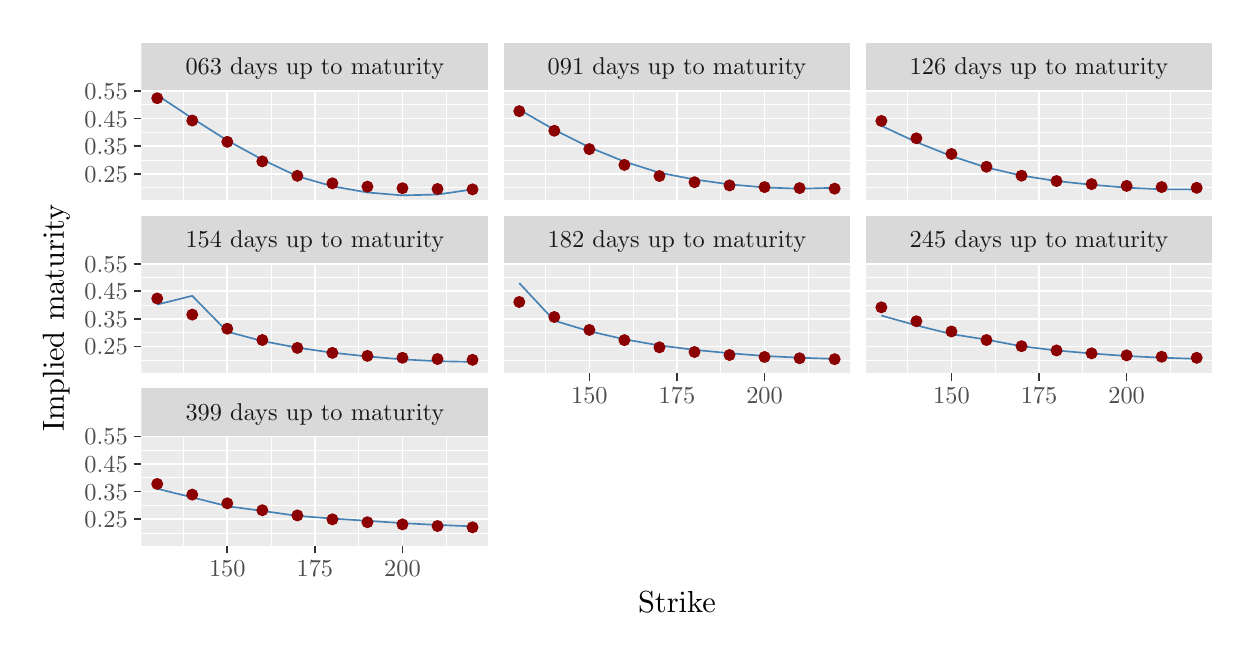
\begin{tikzpicture}[x=1pt,y=1pt]
\definecolor{fillColor}{RGB}{255,255,255}
\path[use as bounding box,fill=fillColor,fill opacity=0.00] (0,0) rectangle (433.62,216.81);
\begin{scope}
\path[clip] (  0.00,  0.00) rectangle (433.62,216.81);
\definecolor{drawColor}{RGB}{255,255,255}
\definecolor{fillColor}{RGB}{255,255,255}

\path[draw=drawColor,line width= 0.6pt,line join=round,line cap=round,fill=fillColor] (  0.00,  0.00) rectangle (433.62,216.81);
\end{scope}
\begin{scope}
\path[clip] ( 41.11,154.40) rectangle (166.45,194.25);
\definecolor{fillColor}{gray}{0.92}

\path[fill=fillColor] ( 41.11,154.40) rectangle (166.45,194.25);
\definecolor{drawColor}{RGB}{255,255,255}

\path[draw=drawColor,line width= 0.3pt,line join=round] ( 41.11,158.99) --
	(166.45,158.99);

\path[draw=drawColor,line width= 0.3pt,line join=round] ( 41.11,168.97) --
	(166.45,168.97);

\path[draw=drawColor,line width= 0.3pt,line join=round] ( 41.11,178.95) --
	(166.45,178.95);

\path[draw=drawColor,line width= 0.3pt,line join=round] ( 41.11,188.93) --
	(166.45,188.93);

\path[draw=drawColor,line width= 0.3pt,line join=round] ( 56.30,154.40) --
	( 56.30,194.25);

\path[draw=drawColor,line width= 0.3pt,line join=round] ( 87.95,154.40) --
	( 87.95,194.25);

\path[draw=drawColor,line width= 0.3pt,line join=round] (119.60,154.40) --
	(119.60,194.25);

\path[draw=drawColor,line width= 0.3pt,line join=round] (151.25,154.40) --
	(151.25,194.25);

\path[draw=drawColor,line width= 0.6pt,line join=round] ( 41.11,163.98) --
	(166.45,163.98);

\path[draw=drawColor,line width= 0.6pt,line join=round] ( 41.11,173.96) --
	(166.45,173.96);

\path[draw=drawColor,line width= 0.6pt,line join=round] ( 41.11,183.94) --
	(166.45,183.94);

\path[draw=drawColor,line width= 0.6pt,line join=round] ( 41.11,193.92) --
	(166.45,193.92);

\path[draw=drawColor,line width= 0.6pt,line join=round] ( 72.13,154.40) --
	( 72.13,194.25);

\path[draw=drawColor,line width= 0.6pt,line join=round] (103.78,154.40) --
	(103.78,194.25);

\path[draw=drawColor,line width= 0.6pt,line join=round] (135.43,154.40) --
	(135.43,194.25);
\definecolor{drawColor}{RGB}{70,130,180}

\path[draw=drawColor,line width= 0.6pt,line join=round] ( 46.81,192.44) --
	( 59.47,184.05) --
	( 72.13,176.06) --
	( 84.79,169.13) --
	( 97.45,163.12) --
	(110.11,159.50) --
	(122.77,157.26) --
	(135.43,156.21) --
	(148.09,156.52) --
	(160.75,158.35);
\definecolor{drawColor}{RGB}{139,0,0}
\definecolor{fillColor}{RGB}{139,0,0}

\path[draw=drawColor,line width= 0.4pt,line join=round,line cap=round,fill=fillColor] ( 46.81,191.32) circle (  1.96);

\path[draw=drawColor,line width= 0.4pt,line join=round,line cap=round,fill=fillColor] ( 59.47,183.25) circle (  1.96);

\path[draw=drawColor,line width= 0.4pt,line join=round,line cap=round,fill=fillColor] ( 72.13,175.56) circle (  1.96);

\path[draw=drawColor,line width= 0.4pt,line join=round,line cap=round,fill=fillColor] ( 84.79,168.49) circle (  1.96);

\path[draw=drawColor,line width= 0.4pt,line join=round,line cap=round,fill=fillColor] ( 97.45,163.27) circle (  1.96);

\path[draw=drawColor,line width= 0.4pt,line join=round,line cap=round,fill=fillColor] (110.11,160.56) circle (  1.96);

\path[draw=drawColor,line width= 0.4pt,line join=round,line cap=round,fill=fillColor] (122.77,159.36) circle (  1.96);

\path[draw=drawColor,line width= 0.4pt,line join=round,line cap=round,fill=fillColor] (135.43,158.80) circle (  1.96);

\path[draw=drawColor,line width= 0.4pt,line join=round,line cap=round,fill=fillColor] (148.09,158.52) circle (  1.96);

\path[draw=drawColor,line width= 0.4pt,line join=round,line cap=round,fill=fillColor] (160.75,158.38) circle (  1.96);
\end{scope}
\begin{scope}
\path[clip] ( 41.11, 91.99) rectangle (166.45,131.84);
\definecolor{fillColor}{gray}{0.92}

\path[fill=fillColor] ( 41.11, 91.99) rectangle (166.45,131.84);
\definecolor{drawColor}{RGB}{255,255,255}

\path[draw=drawColor,line width= 0.3pt,line join=round] ( 41.11, 96.59) --
	(166.45, 96.59);

\path[draw=drawColor,line width= 0.3pt,line join=round] ( 41.11,106.57) --
	(166.45,106.57);

\path[draw=drawColor,line width= 0.3pt,line join=round] ( 41.11,116.55) --
	(166.45,116.55);

\path[draw=drawColor,line width= 0.3pt,line join=round] ( 41.11,126.52) --
	(166.45,126.52);

\path[draw=drawColor,line width= 0.3pt,line join=round] ( 56.30, 91.99) --
	( 56.30,131.84);

\path[draw=drawColor,line width= 0.3pt,line join=round] ( 87.95, 91.99) --
	( 87.95,131.84);

\path[draw=drawColor,line width= 0.3pt,line join=round] (119.60, 91.99) --
	(119.60,131.84);

\path[draw=drawColor,line width= 0.3pt,line join=round] (151.25, 91.99) --
	(151.25,131.84);

\path[draw=drawColor,line width= 0.6pt,line join=round] ( 41.11,101.58) --
	(166.45,101.58);

\path[draw=drawColor,line width= 0.6pt,line join=round] ( 41.11,111.56) --
	(166.45,111.56);

\path[draw=drawColor,line width= 0.6pt,line join=round] ( 41.11,121.54) --
	(166.45,121.54);

\path[draw=drawColor,line width= 0.6pt,line join=round] ( 41.11,131.51) --
	(166.45,131.51);

\path[draw=drawColor,line width= 0.6pt,line join=round] ( 72.13, 91.99) --
	( 72.13,131.84);

\path[draw=drawColor,line width= 0.6pt,line join=round] (103.78, 91.99) --
	(103.78,131.84);

\path[draw=drawColor,line width= 0.6pt,line join=round] (135.43, 91.99) --
	(135.43,131.84);
\definecolor{drawColor}{RGB}{70,130,180}

\path[draw=drawColor,line width= 0.6pt,line join=round] ( 46.81,116.76) --
	( 59.47,119.91) --
	( 72.13,106.96) --
	( 84.79,103.57) --
	( 97.45,101.17) --
	(110.11, 99.36) --
	(122.77, 98.01) --
	(135.43, 96.95) --
	(148.09, 96.29) --
	(160.75, 96.06);
\definecolor{drawColor}{RGB}{139,0,0}
\definecolor{fillColor}{RGB}{139,0,0}

\path[draw=drawColor,line width= 0.4pt,line join=round,line cap=round,fill=fillColor] ( 46.81,118.93) circle (  1.96);

\path[draw=drawColor,line width= 0.4pt,line join=round,line cap=round,fill=fillColor] ( 59.47,113.12) circle (  1.96);

\path[draw=drawColor,line width= 0.4pt,line join=round,line cap=round,fill=fillColor] ( 72.13,108.02) circle (  1.96);

\path[draw=drawColor,line width= 0.4pt,line join=round,line cap=round,fill=fillColor] ( 84.79,103.94) circle (  1.96);

\path[draw=drawColor,line width= 0.4pt,line join=round,line cap=round,fill=fillColor] ( 97.45,101.09) circle (  1.96);

\path[draw=drawColor,line width= 0.4pt,line join=round,line cap=round,fill=fillColor] (110.11, 99.30) circle (  1.96);

\path[draw=drawColor,line width= 0.4pt,line join=round,line cap=round,fill=fillColor] (122.77, 98.21) circle (  1.96);

\path[draw=drawColor,line width= 0.4pt,line join=round,line cap=round,fill=fillColor] (135.43, 97.52) circle (  1.96);

\path[draw=drawColor,line width= 0.4pt,line join=round,line cap=round,fill=fillColor] (148.09, 97.08) circle (  1.96);

\path[draw=drawColor,line width= 0.4pt,line join=round,line cap=round,fill=fillColor] (160.75, 96.78) circle (  1.96);
\end{scope}
\begin{scope}
\path[clip] ( 41.11, 29.59) rectangle (166.45, 69.43);
\definecolor{fillColor}{gray}{0.92}

\path[fill=fillColor] ( 41.11, 29.59) rectangle (166.45, 69.43);
\definecolor{drawColor}{RGB}{255,255,255}

\path[draw=drawColor,line width= 0.3pt,line join=round] ( 41.11, 34.18) --
	(166.45, 34.18);

\path[draw=drawColor,line width= 0.3pt,line join=round] ( 41.11, 44.16) --
	(166.45, 44.16);

\path[draw=drawColor,line width= 0.3pt,line join=round] ( 41.11, 54.14) --
	(166.45, 54.14);

\path[draw=drawColor,line width= 0.3pt,line join=round] ( 41.11, 64.12) --
	(166.45, 64.12);

\path[draw=drawColor,line width= 0.3pt,line join=round] ( 56.30, 29.59) --
	( 56.30, 69.43);

\path[draw=drawColor,line width= 0.3pt,line join=round] ( 87.95, 29.59) --
	( 87.95, 69.43);

\path[draw=drawColor,line width= 0.3pt,line join=round] (119.60, 29.59) --
	(119.60, 69.43);

\path[draw=drawColor,line width= 0.3pt,line join=round] (151.25, 29.59) --
	(151.25, 69.43);

\path[draw=drawColor,line width= 0.6pt,line join=round] ( 41.11, 39.17) --
	(166.45, 39.17);

\path[draw=drawColor,line width= 0.6pt,line join=round] ( 41.11, 49.15) --
	(166.45, 49.15);

\path[draw=drawColor,line width= 0.6pt,line join=round] ( 41.11, 59.13) --
	(166.45, 59.13);

\path[draw=drawColor,line width= 0.6pt,line join=round] ( 41.11, 69.11) --
	(166.45, 69.11);

\path[draw=drawColor,line width= 0.6pt,line join=round] ( 72.13, 29.59) --
	( 72.13, 69.43);

\path[draw=drawColor,line width= 0.6pt,line join=round] (103.78, 29.59) --
	(103.78, 69.43);

\path[draw=drawColor,line width= 0.6pt,line join=round] (135.43, 29.59) --
	(135.43, 69.43);
\definecolor{drawColor}{RGB}{70,130,180}

\path[draw=drawColor,line width= 0.6pt,line join=round] ( 46.81, 50.20) --
	( 59.47, 47.09) --
	( 72.13, 43.89) --
	( 84.79, 42.20) --
	( 97.45, 40.40) --
	(110.11, 39.42) --
	(122.77, 38.61) --
	(135.43, 37.78) --
	(148.09, 37.11) --
	(160.75, 36.62);
\definecolor{drawColor}{RGB}{139,0,0}
\definecolor{fillColor}{RGB}{139,0,0}

\path[draw=drawColor,line width= 0.4pt,line join=round,line cap=round,fill=fillColor] ( 46.81, 51.94) circle (  1.96);

\path[draw=drawColor,line width= 0.4pt,line join=round,line cap=round,fill=fillColor] ( 59.47, 48.07) circle (  1.96);

\path[draw=drawColor,line width= 0.4pt,line join=round,line cap=round,fill=fillColor] ( 72.13, 44.92) circle (  1.96);

\path[draw=drawColor,line width= 0.4pt,line join=round,line cap=round,fill=fillColor] ( 84.79, 42.44) circle (  1.96);

\path[draw=drawColor,line width= 0.4pt,line join=round,line cap=round,fill=fillColor] ( 97.45, 40.56) circle (  1.96);

\path[draw=drawColor,line width= 0.4pt,line join=round,line cap=round,fill=fillColor] (110.11, 39.15) circle (  1.96);

\path[draw=drawColor,line width= 0.4pt,line join=round,line cap=round,fill=fillColor] (122.77, 38.11) circle (  1.96);

\path[draw=drawColor,line width= 0.4pt,line join=round,line cap=round,fill=fillColor] (135.43, 37.32) circle (  1.96);

\path[draw=drawColor,line width= 0.4pt,line join=round,line cap=round,fill=fillColor] (148.09, 36.73) circle (  1.96);

\path[draw=drawColor,line width= 0.4pt,line join=round,line cap=round,fill=fillColor] (160.75, 36.26) circle (  1.96);
\end{scope}
\begin{scope}
\path[clip] (171.95,154.40) rectangle (297.28,194.25);
\definecolor{fillColor}{gray}{0.92}

\path[fill=fillColor] (171.95,154.40) rectangle (297.28,194.25);
\definecolor{drawColor}{RGB}{255,255,255}

\path[draw=drawColor,line width= 0.3pt,line join=round] (171.95,158.99) --
	(297.28,158.99);

\path[draw=drawColor,line width= 0.3pt,line join=round] (171.95,168.97) --
	(297.28,168.97);

\path[draw=drawColor,line width= 0.3pt,line join=round] (171.95,178.95) --
	(297.28,178.95);

\path[draw=drawColor,line width= 0.3pt,line join=round] (171.95,188.93) --
	(297.28,188.93);

\path[draw=drawColor,line width= 0.3pt,line join=round] (187.14,154.40) --
	(187.14,194.25);

\path[draw=drawColor,line width= 0.3pt,line join=round] (218.79,154.40) --
	(218.79,194.25);

\path[draw=drawColor,line width= 0.3pt,line join=round] (250.44,154.40) --
	(250.44,194.25);

\path[draw=drawColor,line width= 0.3pt,line join=round] (282.09,154.40) --
	(282.09,194.25);

\path[draw=drawColor,line width= 0.6pt,line join=round] (171.95,163.98) --
	(297.28,163.98);

\path[draw=drawColor,line width= 0.6pt,line join=round] (171.95,173.96) --
	(297.28,173.96);

\path[draw=drawColor,line width= 0.6pt,line join=round] (171.95,183.94) --
	(297.28,183.94);

\path[draw=drawColor,line width= 0.6pt,line join=round] (171.95,193.92) --
	(297.28,193.92);

\path[draw=drawColor,line width= 0.6pt,line join=round] (202.96,154.40) --
	(202.96,194.25);

\path[draw=drawColor,line width= 0.6pt,line join=round] (234.62,154.40) --
	(234.62,194.25);

\path[draw=drawColor,line width= 0.6pt,line join=round] (266.27,154.40) --
	(266.27,194.25);
\definecolor{drawColor}{RGB}{70,130,180}

\path[draw=drawColor,line width= 0.6pt,line join=round] (177.64,187.21) --
	(190.30,179.91) --
	(202.96,173.56) --
	(215.62,168.42) --
	(228.29,164.40) --
	(240.95,161.96) --
	(253.61,160.18) --
	(266.27,159.07) --
	(278.93,158.62) --
	(291.59,158.94);
\definecolor{drawColor}{RGB}{139,0,0}
\definecolor{fillColor}{RGB}{139,0,0}

\path[draw=drawColor,line width= 0.4pt,line join=round,line cap=round,fill=fillColor] (177.64,186.64) circle (  1.96);

\path[draw=drawColor,line width= 0.4pt,line join=round,line cap=round,fill=fillColor] (190.30,179.55) circle (  1.96);

\path[draw=drawColor,line width= 0.4pt,line join=round,line cap=round,fill=fillColor] (202.96,172.93) circle (  1.96);

\path[draw=drawColor,line width= 0.4pt,line join=round,line cap=round,fill=fillColor] (215.62,167.22) circle (  1.96);

\path[draw=drawColor,line width= 0.4pt,line join=round,line cap=round,fill=fillColor] (228.29,163.21) circle (  1.96);

\path[draw=drawColor,line width= 0.4pt,line join=round,line cap=round,fill=fillColor] (240.95,160.97) circle (  1.96);

\path[draw=drawColor,line width= 0.4pt,line join=round,line cap=round,fill=fillColor] (253.61,159.81) circle (  1.96);

\path[draw=drawColor,line width= 0.4pt,line join=round,line cap=round,fill=fillColor] (266.27,159.20) circle (  1.96);

\path[draw=drawColor,line width= 0.4pt,line join=round,line cap=round,fill=fillColor] (278.93,158.84) circle (  1.96);

\path[draw=drawColor,line width= 0.4pt,line join=round,line cap=round,fill=fillColor] (291.59,158.63) circle (  1.96);
\end{scope}
\begin{scope}
\path[clip] (171.95, 91.99) rectangle (297.28,131.84);
\definecolor{fillColor}{gray}{0.92}

\path[fill=fillColor] (171.95, 91.99) rectangle (297.28,131.84);
\definecolor{drawColor}{RGB}{255,255,255}

\path[draw=drawColor,line width= 0.3pt,line join=round] (171.95, 96.59) --
	(297.28, 96.59);

\path[draw=drawColor,line width= 0.3pt,line join=round] (171.95,106.57) --
	(297.28,106.57);

\path[draw=drawColor,line width= 0.3pt,line join=round] (171.95,116.55) --
	(297.28,116.55);

\path[draw=drawColor,line width= 0.3pt,line join=round] (171.95,126.52) --
	(297.28,126.52);

\path[draw=drawColor,line width= 0.3pt,line join=round] (187.14, 91.99) --
	(187.14,131.84);

\path[draw=drawColor,line width= 0.3pt,line join=round] (218.79, 91.99) --
	(218.79,131.84);

\path[draw=drawColor,line width= 0.3pt,line join=round] (250.44, 91.99) --
	(250.44,131.84);

\path[draw=drawColor,line width= 0.3pt,line join=round] (282.09, 91.99) --
	(282.09,131.84);

\path[draw=drawColor,line width= 0.6pt,line join=round] (171.95,101.58) --
	(297.28,101.58);

\path[draw=drawColor,line width= 0.6pt,line join=round] (171.95,111.56) --
	(297.28,111.56);

\path[draw=drawColor,line width= 0.6pt,line join=round] (171.95,121.54) --
	(297.28,121.54);

\path[draw=drawColor,line width= 0.6pt,line join=round] (171.95,131.51) --
	(297.28,131.51);

\path[draw=drawColor,line width= 0.6pt,line join=round] (202.96, 91.99) --
	(202.96,131.84);

\path[draw=drawColor,line width= 0.6pt,line join=round] (234.62, 91.99) --
	(234.62,131.84);

\path[draw=drawColor,line width= 0.6pt,line join=round] (266.27, 91.99) --
	(266.27,131.84);
\definecolor{drawColor}{RGB}{70,130,180}

\path[draw=drawColor,line width= 0.6pt,line join=round] (177.64,124.51) --
	(190.30,110.93) --
	(202.96,107.13) --
	(215.62,104.20) --
	(228.29,101.98) --
	(240.95,100.40) --
	(253.61, 99.17) --
	(266.27, 98.18) --
	(278.93, 97.55) --
	(291.59, 97.12);
\definecolor{drawColor}{RGB}{139,0,0}
\definecolor{fillColor}{RGB}{139,0,0}

\path[draw=drawColor,line width= 0.4pt,line join=round,line cap=round,fill=fillColor] (177.64,117.69) circle (  1.96);

\path[draw=drawColor,line width= 0.4pt,line join=round,line cap=round,fill=fillColor] (190.30,112.26) circle (  1.96);

\path[draw=drawColor,line width= 0.4pt,line join=round,line cap=round,fill=fillColor] (202.96,107.59) circle (  1.96);

\path[draw=drawColor,line width= 0.4pt,line join=round,line cap=round,fill=fillColor] (215.62,103.90) circle (  1.96);

\path[draw=drawColor,line width= 0.4pt,line join=round,line cap=round,fill=fillColor] (228.29,101.30) circle (  1.96);

\path[draw=drawColor,line width= 0.4pt,line join=round,line cap=round,fill=fillColor] (240.95, 99.61) circle (  1.96);

\path[draw=drawColor,line width= 0.4pt,line join=round,line cap=round,fill=fillColor] (253.61, 98.52) circle (  1.96);

\path[draw=drawColor,line width= 0.4pt,line join=round,line cap=round,fill=fillColor] (266.27, 97.82) circle (  1.96);

\path[draw=drawColor,line width= 0.4pt,line join=round,line cap=round,fill=fillColor] (278.93, 97.35) circle (  1.96);

\path[draw=drawColor,line width= 0.4pt,line join=round,line cap=round,fill=fillColor] (291.59, 97.02) circle (  1.96);
\end{scope}
\begin{scope}
\path[clip] (302.78,154.40) rectangle (428.12,194.25);
\definecolor{fillColor}{gray}{0.92}

\path[fill=fillColor] (302.78,154.40) rectangle (428.12,194.25);
\definecolor{drawColor}{RGB}{255,255,255}

\path[draw=drawColor,line width= 0.3pt,line join=round] (302.78,158.99) --
	(428.12,158.99);

\path[draw=drawColor,line width= 0.3pt,line join=round] (302.78,168.97) --
	(428.12,168.97);

\path[draw=drawColor,line width= 0.3pt,line join=round] (302.78,178.95) --
	(428.12,178.95);

\path[draw=drawColor,line width= 0.3pt,line join=round] (302.78,188.93) --
	(428.12,188.93);

\path[draw=drawColor,line width= 0.3pt,line join=round] (317.98,154.40) --
	(317.98,194.25);

\path[draw=drawColor,line width= 0.3pt,line join=round] (349.63,154.40) --
	(349.63,194.25);

\path[draw=drawColor,line width= 0.3pt,line join=round] (381.28,154.40) --
	(381.28,194.25);

\path[draw=drawColor,line width= 0.3pt,line join=round] (412.93,154.40) --
	(412.93,194.25);

\path[draw=drawColor,line width= 0.6pt,line join=round] (302.78,163.98) --
	(428.12,163.98);

\path[draw=drawColor,line width= 0.6pt,line join=round] (302.78,173.96) --
	(428.12,173.96);

\path[draw=drawColor,line width= 0.6pt,line join=round] (302.78,183.94) --
	(428.12,183.94);

\path[draw=drawColor,line width= 0.6pt,line join=round] (302.78,193.92) --
	(428.12,193.92);

\path[draw=drawColor,line width= 0.6pt,line join=round] (333.80,154.40) --
	(333.80,194.25);

\path[draw=drawColor,line width= 0.6pt,line join=round] (365.45,154.40) --
	(365.45,194.25);

\path[draw=drawColor,line width= 0.6pt,line join=round] (397.10,154.40) --
	(397.10,194.25);
\definecolor{drawColor}{RGB}{70,130,180}

\path[draw=drawColor,line width= 0.6pt,line join=round] (308.48,181.34) --
	(321.14,175.45) --
	(333.80,170.41) --
	(346.46,166.28) --
	(359.12,163.37) --
	(371.78,161.38) --
	(384.44,160.05) --
	(397.10,158.99) --
	(409.76,158.40) --
	(422.42,158.35);
\definecolor{drawColor}{RGB}{139,0,0}
\definecolor{fillColor}{RGB}{139,0,0}

\path[draw=drawColor,line width= 0.4pt,line join=round,line cap=round,fill=fillColor] (308.48,183.11) circle (  1.96);

\path[draw=drawColor,line width= 0.4pt,line join=round,line cap=round,fill=fillColor] (321.14,176.83) circle (  1.96);

\path[draw=drawColor,line width= 0.4pt,line join=round,line cap=round,fill=fillColor] (333.80,171.17) circle (  1.96);

\path[draw=drawColor,line width= 0.4pt,line join=round,line cap=round,fill=fillColor] (346.46,166.54) circle (  1.96);

\path[draw=drawColor,line width= 0.4pt,line join=round,line cap=round,fill=fillColor] (359.12,163.32) circle (  1.96);

\path[draw=drawColor,line width= 0.4pt,line join=round,line cap=round,fill=fillColor] (371.78,161.39) circle (  1.96);

\path[draw=drawColor,line width= 0.4pt,line join=round,line cap=round,fill=fillColor] (384.44,160.28) circle (  1.96);

\path[draw=drawColor,line width= 0.4pt,line join=round,line cap=round,fill=fillColor] (397.10,159.62) circle (  1.96);

\path[draw=drawColor,line width= 0.4pt,line join=round,line cap=round,fill=fillColor] (409.76,159.21) circle (  1.96);

\path[draw=drawColor,line width= 0.4pt,line join=round,line cap=round,fill=fillColor] (422.42,158.94) circle (  1.96);
\end{scope}
\begin{scope}
\path[clip] (302.78, 91.99) rectangle (428.12,131.84);
\definecolor{fillColor}{gray}{0.92}

\path[fill=fillColor] (302.78, 91.99) rectangle (428.12,131.84);
\definecolor{drawColor}{RGB}{255,255,255}

\path[draw=drawColor,line width= 0.3pt,line join=round] (302.78, 96.59) --
	(428.12, 96.59);

\path[draw=drawColor,line width= 0.3pt,line join=round] (302.78,106.57) --
	(428.12,106.57);

\path[draw=drawColor,line width= 0.3pt,line join=round] (302.78,116.55) --
	(428.12,116.55);

\path[draw=drawColor,line width= 0.3pt,line join=round] (302.78,126.52) --
	(428.12,126.52);

\path[draw=drawColor,line width= 0.3pt,line join=round] (317.98, 91.99) --
	(317.98,131.84);

\path[draw=drawColor,line width= 0.3pt,line join=round] (349.63, 91.99) --
	(349.63,131.84);

\path[draw=drawColor,line width= 0.3pt,line join=round] (381.28, 91.99) --
	(381.28,131.84);

\path[draw=drawColor,line width= 0.3pt,line join=round] (412.93, 91.99) --
	(412.93,131.84);

\path[draw=drawColor,line width= 0.6pt,line join=round] (302.78,101.58) --
	(428.12,101.58);

\path[draw=drawColor,line width= 0.6pt,line join=round] (302.78,111.56) --
	(428.12,111.56);

\path[draw=drawColor,line width= 0.6pt,line join=round] (302.78,121.54) --
	(428.12,121.54);

\path[draw=drawColor,line width= 0.6pt,line join=round] (302.78,131.51) --
	(428.12,131.51);

\path[draw=drawColor,line width= 0.6pt,line join=round] (333.80, 91.99) --
	(333.80,131.84);

\path[draw=drawColor,line width= 0.6pt,line join=round] (365.45, 91.99) --
	(365.45,131.84);

\path[draw=drawColor,line width= 0.6pt,line join=round] (397.10, 91.99) --
	(397.10,131.84);
\definecolor{drawColor}{RGB}{70,130,180}

\path[draw=drawColor,line width= 0.6pt,line join=round] (308.48,112.77) --
	(321.14,109.24) --
	(333.80,106.08) --
	(346.46,104.08) --
	(359.12,101.69) --
	(371.78,100.16) --
	(384.44, 99.08) --
	(397.10, 98.16) --
	(409.76, 97.55) --
	(422.42, 97.14);
\definecolor{drawColor}{RGB}{139,0,0}
\definecolor{fillColor}{RGB}{139,0,0}

\path[draw=drawColor,line width= 0.4pt,line join=round,line cap=round,fill=fillColor] (308.48,115.75) circle (  1.96);

\path[draw=drawColor,line width= 0.4pt,line join=round,line cap=round,fill=fillColor] (321.14,110.73) circle (  1.96);

\path[draw=drawColor,line width= 0.4pt,line join=round,line cap=round,fill=fillColor] (333.80,107.03) circle (  1.96);

\path[draw=drawColor,line width= 0.4pt,line join=round,line cap=round,fill=fillColor] (346.46,103.94) circle (  1.96);

\path[draw=drawColor,line width= 0.4pt,line join=round,line cap=round,fill=fillColor] (359.12,101.71) circle (  1.96);

\path[draw=drawColor,line width= 0.4pt,line join=round,line cap=round,fill=fillColor] (371.78,100.18) circle (  1.96);

\path[draw=drawColor,line width= 0.4pt,line join=round,line cap=round,fill=fillColor] (384.44, 99.13) circle (  1.96);

\path[draw=drawColor,line width= 0.4pt,line join=round,line cap=round,fill=fillColor] (397.10, 98.40) circle (  1.96);

\path[draw=drawColor,line width= 0.4pt,line join=round,line cap=round,fill=fillColor] (409.76, 97.89) circle (  1.96);

\path[draw=drawColor,line width= 0.4pt,line join=round,line cap=round,fill=fillColor] (422.42, 97.51) circle (  1.96);
\end{scope}
\begin{scope}
\path[clip] ( 41.11, 69.43) rectangle (166.45, 86.49);
\definecolor{fillColor}{gray}{0.85}

\path[fill=fillColor] ( 41.11, 69.43) rectangle (166.45, 86.49);
\definecolor{drawColor}{gray}{0.10}

\node[text=drawColor,anchor=base,inner sep=0pt, outer sep=0pt, scale=  0.88] at (103.78, 74.93) {399 days up to maturity};
\end{scope}
\begin{scope}
\path[clip] ( 41.11,131.84) rectangle (166.45,148.90);
\definecolor{fillColor}{gray}{0.85}

\path[fill=fillColor] ( 41.11,131.84) rectangle (166.45,148.90);
\definecolor{drawColor}{gray}{0.10}

\node[text=drawColor,anchor=base,inner sep=0pt, outer sep=0pt, scale=  0.88] at (103.78,137.34) {154 days up to maturity};
\end{scope}
\begin{scope}
\path[clip] (171.95,131.84) rectangle (297.28,148.90);
\definecolor{fillColor}{gray}{0.85}

\path[fill=fillColor] (171.95,131.84) rectangle (297.28,148.90);
\definecolor{drawColor}{gray}{0.10}

\node[text=drawColor,anchor=base,inner sep=0pt, outer sep=0pt, scale=  0.88] at (234.62,137.34) {182 days up to maturity};
\end{scope}
\begin{scope}
\path[clip] (302.78,131.84) rectangle (428.12,148.90);
\definecolor{fillColor}{gray}{0.85}

\path[fill=fillColor] (302.78,131.84) rectangle (428.12,148.90);
\definecolor{drawColor}{gray}{0.10}

\node[text=drawColor,anchor=base,inner sep=0pt, outer sep=0pt, scale=  0.88] at (365.45,137.34) {245 days up to maturity};
\end{scope}
\begin{scope}
\path[clip] ( 41.11,194.25) rectangle (166.45,211.31);
\definecolor{fillColor}{gray}{0.85}

\path[fill=fillColor] ( 41.11,194.25) rectangle (166.45,211.31);
\definecolor{drawColor}{gray}{0.10}

\node[text=drawColor,anchor=base,inner sep=0pt, outer sep=0pt, scale=  0.88] at (103.78,199.75) {063 days up to maturity};
\end{scope}
\begin{scope}
\path[clip] (171.95,194.25) rectangle (297.28,211.31);
\definecolor{fillColor}{gray}{0.85}

\path[fill=fillColor] (171.95,194.25) rectangle (297.28,211.31);
\definecolor{drawColor}{gray}{0.10}

\node[text=drawColor,anchor=base,inner sep=0pt, outer sep=0pt, scale=  0.88] at (234.62,199.75) {091 days up to maturity};
\end{scope}
\begin{scope}
\path[clip] (302.78,194.25) rectangle (428.12,211.31);
\definecolor{fillColor}{gray}{0.85}

\path[fill=fillColor] (302.78,194.25) rectangle (428.12,211.31);
\definecolor{drawColor}{gray}{0.10}

\node[text=drawColor,anchor=base,inner sep=0pt, outer sep=0pt, scale=  0.88] at (365.45,199.75) {126 days up to maturity};
\end{scope}
\begin{scope}
\path[clip] (  0.00,  0.00) rectangle (433.62,216.81);
\definecolor{drawColor}{gray}{0.20}

\path[draw=drawColor,line width= 0.6pt,line join=round] ( 72.13, 26.84) --
	( 72.13, 29.59);

\path[draw=drawColor,line width= 0.6pt,line join=round] (103.78, 26.84) --
	(103.78, 29.59);

\path[draw=drawColor,line width= 0.6pt,line join=round] (135.43, 26.84) --
	(135.43, 29.59);
\end{scope}
\begin{scope}
\path[clip] (  0.00,  0.00) rectangle (433.62,216.81);
\definecolor{drawColor}{gray}{0.30}

\node[text=drawColor,anchor=base,inner sep=0pt, outer sep=0pt, scale=  0.88] at ( 72.13, 18.58) {150};

\node[text=drawColor,anchor=base,inner sep=0pt, outer sep=0pt, scale=  0.88] at (103.78, 18.58) {175};

\node[text=drawColor,anchor=base,inner sep=0pt, outer sep=0pt, scale=  0.88] at (135.43, 18.58) {200};
\end{scope}
\begin{scope}
\path[clip] (  0.00,  0.00) rectangle (433.62,216.81);
\definecolor{drawColor}{gray}{0.20}

\path[draw=drawColor,line width= 0.6pt,line join=round] (202.96, 89.24) --
	(202.96, 91.99);

\path[draw=drawColor,line width= 0.6pt,line join=round] (234.62, 89.24) --
	(234.62, 91.99);

\path[draw=drawColor,line width= 0.6pt,line join=round] (266.27, 89.24) --
	(266.27, 91.99);
\end{scope}
\begin{scope}
\path[clip] (  0.00,  0.00) rectangle (433.62,216.81);
\definecolor{drawColor}{gray}{0.30}

\node[text=drawColor,anchor=base,inner sep=0pt, outer sep=0pt, scale=  0.88] at (202.96, 80.98) {150};

\node[text=drawColor,anchor=base,inner sep=0pt, outer sep=0pt, scale=  0.88] at (234.62, 80.98) {175};

\node[text=drawColor,anchor=base,inner sep=0pt, outer sep=0pt, scale=  0.88] at (266.27, 80.98) {200};
\end{scope}
\begin{scope}
\path[clip] (  0.00,  0.00) rectangle (433.62,216.81);
\definecolor{drawColor}{gray}{0.20}

\path[draw=drawColor,line width= 0.6pt,line join=round] (333.80, 89.24) --
	(333.80, 91.99);

\path[draw=drawColor,line width= 0.6pt,line join=round] (365.45, 89.24) --
	(365.45, 91.99);

\path[draw=drawColor,line width= 0.6pt,line join=round] (397.10, 89.24) --
	(397.10, 91.99);
\end{scope}
\begin{scope}
\path[clip] (  0.00,  0.00) rectangle (433.62,216.81);
\definecolor{drawColor}{gray}{0.30}

\node[text=drawColor,anchor=base,inner sep=0pt, outer sep=0pt, scale=  0.88] at (333.80, 80.98) {150};

\node[text=drawColor,anchor=base,inner sep=0pt, outer sep=0pt, scale=  0.88] at (365.45, 80.98) {175};

\node[text=drawColor,anchor=base,inner sep=0pt, outer sep=0pt, scale=  0.88] at (397.10, 80.98) {200};
\end{scope}
\begin{scope}
\path[clip] (  0.00,  0.00) rectangle (433.62,216.81);
\definecolor{drawColor}{gray}{0.30}

\node[text=drawColor,anchor=base east,inner sep=0pt, outer sep=0pt, scale=  0.88] at ( 36.16,160.95) {0.25};

\node[text=drawColor,anchor=base east,inner sep=0pt, outer sep=0pt, scale=  0.88] at ( 36.16,170.93) {0.35};

\node[text=drawColor,anchor=base east,inner sep=0pt, outer sep=0pt, scale=  0.88] at ( 36.16,180.91) {0.45};

\node[text=drawColor,anchor=base east,inner sep=0pt, outer sep=0pt, scale=  0.88] at ( 36.16,190.89) {0.55};
\end{scope}
\begin{scope}
\path[clip] (  0.00,  0.00) rectangle (433.62,216.81);
\definecolor{drawColor}{gray}{0.20}

\path[draw=drawColor,line width= 0.6pt,line join=round] ( 38.36,163.98) --
	( 41.11,163.98);

\path[draw=drawColor,line width= 0.6pt,line join=round] ( 38.36,173.96) --
	( 41.11,173.96);

\path[draw=drawColor,line width= 0.6pt,line join=round] ( 38.36,183.94) --
	( 41.11,183.94);

\path[draw=drawColor,line width= 0.6pt,line join=round] ( 38.36,193.92) --
	( 41.11,193.92);
\end{scope}
\begin{scope}
\path[clip] (  0.00,  0.00) rectangle (433.62,216.81);
\definecolor{drawColor}{gray}{0.30}

\node[text=drawColor,anchor=base east,inner sep=0pt, outer sep=0pt, scale=  0.88] at ( 36.16, 98.55) {0.25};

\node[text=drawColor,anchor=base east,inner sep=0pt, outer sep=0pt, scale=  0.88] at ( 36.16,108.52) {0.35};

\node[text=drawColor,anchor=base east,inner sep=0pt, outer sep=0pt, scale=  0.88] at ( 36.16,118.50) {0.45};

\node[text=drawColor,anchor=base east,inner sep=0pt, outer sep=0pt, scale=  0.88] at ( 36.16,128.48) {0.55};
\end{scope}
\begin{scope}
\path[clip] (  0.00,  0.00) rectangle (433.62,216.81);
\definecolor{drawColor}{gray}{0.20}

\path[draw=drawColor,line width= 0.6pt,line join=round] ( 38.36,101.58) --
	( 41.11,101.58);

\path[draw=drawColor,line width= 0.6pt,line join=round] ( 38.36,111.56) --
	( 41.11,111.56);

\path[draw=drawColor,line width= 0.6pt,line join=round] ( 38.36,121.54) --
	( 41.11,121.54);

\path[draw=drawColor,line width= 0.6pt,line join=round] ( 38.36,131.51) --
	( 41.11,131.51);
\end{scope}
\begin{scope}
\path[clip] (  0.00,  0.00) rectangle (433.62,216.81);
\definecolor{drawColor}{gray}{0.30}

\node[text=drawColor,anchor=base east,inner sep=0pt, outer sep=0pt, scale=  0.88] at ( 36.16, 36.14) {0.25};

\node[text=drawColor,anchor=base east,inner sep=0pt, outer sep=0pt, scale=  0.88] at ( 36.16, 46.12) {0.35};

\node[text=drawColor,anchor=base east,inner sep=0pt, outer sep=0pt, scale=  0.88] at ( 36.16, 56.10) {0.45};

\node[text=drawColor,anchor=base east,inner sep=0pt, outer sep=0pt, scale=  0.88] at ( 36.16, 66.08) {0.55};
\end{scope}
\begin{scope}
\path[clip] (  0.00,  0.00) rectangle (433.62,216.81);
\definecolor{drawColor}{gray}{0.20}

\path[draw=drawColor,line width= 0.6pt,line join=round] ( 38.36, 39.17) --
	( 41.11, 39.17);

\path[draw=drawColor,line width= 0.6pt,line join=round] ( 38.36, 49.15) --
	( 41.11, 49.15);

\path[draw=drawColor,line width= 0.6pt,line join=round] ( 38.36, 59.13) --
	( 41.11, 59.13);

\path[draw=drawColor,line width= 0.6pt,line join=round] ( 38.36, 69.11) --
	( 41.11, 69.11);
\end{scope}
\begin{scope}
\path[clip] (  0.00,  0.00) rectangle (433.62,216.81);
\definecolor{drawColor}{RGB}{0,0,0}

\node[text=drawColor,anchor=base,inner sep=0pt, outer sep=0pt, scale=  1.10] at (234.62,  5.50) {Strike};
\end{scope}
\begin{scope}
\path[clip] (  0.00,  0.00) rectangle (433.62,216.81);
\definecolor{drawColor}{RGB}{0,0,0}

\node[text=drawColor,rotate= 90.00,anchor=base,inner sep=0pt, outer sep=0pt, scale=  1.10] at ( 13.08,111.92) {Implied maturity};
\end{scope}
\end{tikzpicture}

  \caption{Implied volatility of Apple option prices computed with MJD} 
   \floatfoot{\textbf{Notes.} The implied volatilities that represent the above volatility smiles have been computed by using an iterative method on the BSM equation to solve  $\sigma$.
  The parameters given to the function \textit{bsm\_call} were the stock price $S$, the strike price $K$, the riskless rate $r$ and the time to maturity $T$, letting $\sigma$ unknown.
  The method used was to find the root of $C(S(0), K, T, r; \sigma) - C_{K, T}$, where $C_{K, T}$ is either the market price or the price giving by the function \textit{mjd\_call}, and $C(S(0), K, T, r; \sigma)$ is the function \textit{bsm\_call} with $\sigma$ as a cursor.}
  \label{p:methodology:impliedvol:aapl:merton}
\end{figure}


Consequently, for the purpose of that master thesis, the set \ref{eq:methodology:arg:merton:riskneutral} is the one that will be used together with the function \textit{mjd\_call} whenever performing the computation of option prices for the MJD model.





%%%%%%%%%%%%%%%%%%%%%%%%%%%%%%%%%%%%%%%%%%%%%%%%%%%%%%%%%%%%%%%%%%%%%%%%%%%%%%%%
\subsubsection*{Calibration of parameters for time series}

The set \ref{eq:methodology:arg:merton:riskneutral} is calibrated under the risk-neutral world and cannot, therefore, be used as is to simulate the dummy time-series that will serve the analysis aimed to measure the delta hedging performance.
Furthermore, in addition to those parameters, the drift rate $\alpha$ has to be estimated as well. It was not present in the set  \ref{eq:methodology:arg:merton:riskneutral} because it was not taken into account in the computation of the options prices.

\Cref{p:methodology:density:aapl:merton:riskneutral} shows the empirical density curves illustrating the distributions of the log-returns computed either from historical Apple stock data for the blue curve or from dummy time series generated by the function \textit{mjd\_ts()} fed with the risk-neutral parameters\ref{eq:methodology:arg:merton:riskneutral}, for the red one.


\begin{figure}[ht]
  \centering
  % Created by tikzDevice version 0.11 on 2018-07-21 23:11:46
% !TEX encoding = UTF-8 Unicode
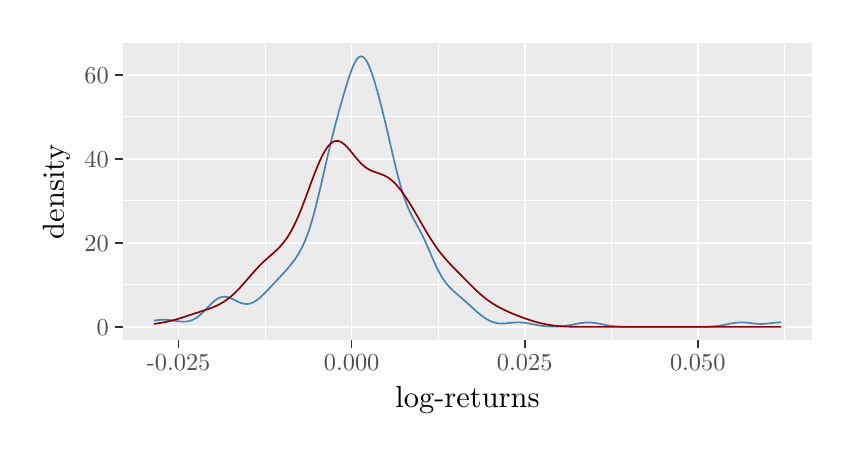
\begin{tikzpicture}[x=1pt,y=1pt]
\definecolor{fillColor}{RGB}{255,255,255}
\path[use as bounding box,fill=fillColor,fill opacity=0.00] (0,0) rectangle (289.08,144.54);
\begin{scope}
\path[clip] (  0.00,  0.00) rectangle (289.08,144.54);
\definecolor{drawColor}{RGB}{255,255,255}
\definecolor{fillColor}{RGB}{255,255,255}

\path[draw=drawColor,line width= 0.6pt,line join=round,line cap=round,fill=fillColor] (  0.00,  0.00) rectangle (289.08,144.54);
\end{scope}
\begin{scope}
\path[clip] ( 34.27, 31.53) rectangle (283.58,139.04);
\definecolor{fillColor}{gray}{0.92}

\path[fill=fillColor] ( 34.27, 31.53) rectangle (283.58,139.04);
\definecolor{drawColor}{RGB}{255,255,255}

\path[draw=drawColor,line width= 0.3pt,line join=round] ( 34.27, 51.60) --
	(283.58, 51.60);

\path[draw=drawColor,line width= 0.3pt,line join=round] ( 34.27, 81.97) --
	(283.58, 81.97);

\path[draw=drawColor,line width= 0.3pt,line join=round] ( 34.27,112.33) --
	(283.58,112.33);

\path[draw=drawColor,line width= 0.3pt,line join=round] ( 85.80, 31.53) --
	( 85.80,139.04);

\path[draw=drawColor,line width= 0.3pt,line join=round] (148.33, 31.53) --
	(148.33,139.04);

\path[draw=drawColor,line width= 0.3pt,line join=round] (210.86, 31.53) --
	(210.86,139.04);

\path[draw=drawColor,line width= 0.3pt,line join=round] (273.40, 31.53) --
	(273.40,139.04);

\path[draw=drawColor,line width= 0.6pt,line join=round] ( 34.27, 36.42) --
	(283.58, 36.42);

\path[draw=drawColor,line width= 0.6pt,line join=round] ( 34.27, 66.78) --
	(283.58, 66.78);

\path[draw=drawColor,line width= 0.6pt,line join=round] ( 34.27, 97.15) --
	(283.58, 97.15);

\path[draw=drawColor,line width= 0.6pt,line join=round] ( 34.27,127.52) --
	(283.58,127.52);

\path[draw=drawColor,line width= 0.6pt,line join=round] ( 54.53, 31.53) --
	( 54.53,139.04);

\path[draw=drawColor,line width= 0.6pt,line join=round] (117.07, 31.53) --
	(117.07,139.04);

\path[draw=drawColor,line width= 0.6pt,line join=round] (179.60, 31.53) --
	(179.60,139.04);

\path[draw=drawColor,line width= 0.6pt,line join=round] (242.13, 31.53) --
	(242.13,139.04);
\definecolor{drawColor}{RGB}{70,130,180}

\path[draw=drawColor,line width= 0.6pt,line join=round] ( 45.60, 38.68) --
	( 46.04, 38.76) --
	( 46.49, 38.82) --
	( 46.93, 38.88) --
	( 47.37, 38.92) --
	( 47.82, 38.96) --
	( 48.26, 38.98) --
	( 48.70, 39.00) --
	( 49.15, 39.00) --
	( 49.59, 38.99) --
	( 50.04, 38.97) --
	( 50.48, 38.94) --
	( 50.92, 38.90) --
	( 51.37, 38.86) --
	( 51.81, 38.81) --
	( 52.25, 38.75) --
	( 52.70, 38.69) --
	( 53.14, 38.62) --
	( 53.58, 38.56) --
	( 54.03, 38.50) --
	( 54.47, 38.44) --
	( 54.91, 38.39) --
	( 55.36, 38.35) --
	( 55.80, 38.32) --
	( 56.25, 38.30) --
	( 56.69, 38.31) --
	( 57.13, 38.33) --
	( 57.58, 38.38) --
	( 58.02, 38.46) --
	( 58.46, 38.56) --
	( 58.91, 38.68) --
	( 59.35, 38.85) --
	( 59.79, 39.04) --
	( 60.24, 39.27) --
	( 60.68, 39.53) --
	( 61.12, 39.82) --
	( 61.57, 40.14) --
	( 62.01, 40.49) --
	( 62.45, 40.87) --
	( 62.90, 41.27) --
	( 63.34, 41.70) --
	( 63.79, 42.14) --
	( 64.23, 42.59) --
	( 64.67, 43.05) --
	( 65.12, 43.52) --
	( 65.56, 43.98) --
	( 66.00, 44.43) --
	( 66.45, 44.86) --
	( 66.89, 45.28) --
	( 67.33, 45.67) --
	( 67.78, 46.03) --
	( 68.22, 46.35) --
	( 68.66, 46.62) --
	( 69.11, 46.85) --
	( 69.55, 47.04) --
	( 69.99, 47.17) --
	( 70.44, 47.27) --
	( 70.88, 47.31) --
	( 71.33, 47.30) --
	( 71.77, 47.25) --
	( 72.21, 47.15) --
	( 72.66, 47.03) --
	( 73.10, 46.87) --
	( 73.54, 46.69) --
	( 73.99, 46.49) --
	( 74.43, 46.27) --
	( 74.87, 46.05) --
	( 75.32, 45.83) --
	( 75.76, 45.61) --
	( 76.20, 45.41) --
	( 76.65, 45.22) --
	( 77.09, 45.05) --
	( 77.53, 44.91) --
	( 77.98, 44.81) --
	( 78.42, 44.73) --
	( 78.87, 44.70) --
	( 79.31, 44.70) --
	( 79.75, 44.73) --
	( 80.20, 44.81) --
	( 80.64, 44.94) --
	( 81.08, 45.10) --
	( 81.53, 45.30) --
	( 81.97, 45.54) --
	( 82.41, 45.81) --
	( 82.86, 46.11) --
	( 83.30, 46.45) --
	( 83.74, 46.81) --
	( 84.19, 47.20) --
	( 84.63, 47.61) --
	( 85.07, 48.04) --
	( 85.52, 48.48) --
	( 85.96, 48.93) --
	( 86.41, 49.39) --
	( 86.85, 49.85) --
	( 87.29, 50.32) --
	( 87.74, 50.80) --
	( 88.18, 51.27) --
	( 88.62, 51.74) --
	( 89.07, 52.22) --
	( 89.51, 52.69) --
	( 89.95, 53.16) --
	( 90.40, 53.63) --
	( 90.84, 54.11) --
	( 91.28, 54.58) --
	( 91.73, 55.06) --
	( 92.17, 55.54) --
	( 92.62, 56.02) --
	( 93.06, 56.51) --
	( 93.50, 57.01) --
	( 93.95, 57.52) --
	( 94.39, 58.04) --
	( 94.83, 58.57) --
	( 95.28, 59.12) --
	( 95.72, 59.68) --
	( 96.16, 60.28) --
	( 96.61, 60.89) --
	( 97.05, 61.54) --
	( 97.49, 62.22) --
	( 97.94, 62.94) --
	( 98.38, 63.71) --
	( 98.82, 64.54) --
	( 99.27, 65.42) --
	( 99.71, 66.36) --
	(100.16, 67.37) --
	(100.60, 68.45) --
	(101.04, 69.61) --
	(101.49, 70.85) --
	(101.93, 72.18) --
	(102.37, 73.59) --
	(102.82, 75.08) --
	(103.26, 76.64) --
	(103.70, 78.28) --
	(104.15, 79.99) --
	(104.59, 81.77) --
	(105.03, 83.60) --
	(105.48, 85.48) --
	(105.92, 87.38) --
	(106.36, 89.32) --
	(106.81, 91.26) --
	(107.25, 93.21) --
	(107.70, 95.15) --
	(108.14, 97.08) --
	(108.58, 98.98) --
	(109.03,100.86) --
	(109.47,102.71) --
	(109.91,104.52) --
	(110.36,106.30) --
	(110.80,108.04) --
	(111.24,109.74) --
	(111.69,111.42) --
	(112.13,113.06) --
	(112.57,114.69) --
	(113.02,116.28) --
	(113.46,117.86) --
	(113.90,119.41) --
	(114.35,120.93) --
	(114.79,122.43) --
	(115.24,123.88) --
	(115.68,125.30) --
	(116.12,126.66) --
	(116.57,127.96) --
	(117.01,129.16) --
	(117.45,130.26) --
	(117.90,131.26) --
	(118.34,132.13) --
	(118.78,132.86) --
	(119.23,133.45) --
	(119.67,133.87) --
	(120.11,134.10) --
	(120.56,134.15) --
	(121.00,134.04) --
	(121.45,133.76) --
	(121.89,133.31) --
	(122.33,132.70) --
	(122.78,131.92) --
	(123.22,130.99) --
	(123.66,129.94) --
	(124.11,128.77) --
	(124.55,127.51) --
	(124.99,126.15) --
	(125.44,124.72) --
	(125.88,123.20) --
	(126.32,121.63) --
	(126.77,120.00) --
	(127.21,118.33) --
	(127.65,116.61) --
	(128.10,114.85) --
	(128.54,113.06) --
	(128.99,111.23) --
	(129.43,109.37) --
	(129.87,107.49) --
	(130.32,105.59) --
	(130.76,103.68) --
	(131.20,101.75) --
	(131.65, 99.83) --
	(132.09, 97.93) --
	(132.53, 96.05) --
	(132.98, 94.21) --
	(133.42, 92.41) --
	(133.86, 90.67) --
	(134.31, 88.99) --
	(134.75, 87.39) --
	(135.19, 85.88) --
	(135.64, 84.45) --
	(136.08, 83.11) --
	(136.53, 81.86) --
	(136.97, 80.69) --
	(137.41, 79.60) --
	(137.86, 78.58) --
	(138.30, 77.64) --
	(138.74, 76.74) --
	(139.19, 75.89) --
	(139.63, 75.06) --
	(140.07, 74.26) --
	(140.52, 73.46) --
	(140.96, 72.65) --
	(141.40, 71.83) --
	(141.85, 70.99) --
	(142.29, 70.13) --
	(142.73, 69.23) --
	(143.18, 68.31) --
	(143.62, 67.36) --
	(144.07, 66.37) --
	(144.51, 65.37) --
	(144.95, 64.35) --
	(145.40, 63.32) --
	(145.84, 62.29) --
	(146.28, 61.27) --
	(146.73, 60.26) --
	(147.17, 59.28) --
	(147.61, 58.32) --
	(148.06, 57.41) --
	(148.50, 56.54) --
	(148.94, 55.70) --
	(149.39, 54.92) --
	(149.83, 54.18) --
	(150.27, 53.50) --
	(150.72, 52.87) --
	(151.16, 52.28) --
	(151.61, 51.72) --
	(152.05, 51.21) --
	(152.49, 50.72) --
	(152.94, 50.27) --
	(153.38, 49.84) --
	(153.82, 49.43) --
	(154.27, 49.03) --
	(154.71, 48.64) --
	(155.15, 48.26) --
	(155.60, 47.88) --
	(156.04, 47.50) --
	(156.48, 47.12) --
	(156.93, 46.73) --
	(157.37, 46.34) --
	(157.82, 45.95) --
	(158.26, 45.56) --
	(158.70, 45.16) --
	(159.15, 44.75) --
	(159.59, 44.35) --
	(160.03, 43.94) --
	(160.48, 43.54) --
	(160.92, 43.13) --
	(161.36, 42.74) --
	(161.81, 42.34) --
	(162.25, 41.95) --
	(162.69, 41.57) --
	(163.14, 41.21) --
	(163.58, 40.85) --
	(164.02, 40.50) --
	(164.47, 40.17) --
	(164.91, 39.86) --
	(165.36, 39.56) --
	(165.80, 39.28) --
	(166.24, 39.03) --
	(166.69, 38.79) --
	(167.13, 38.57) --
	(167.57, 38.38) --
	(168.02, 38.21) --
	(168.46, 38.06) --
	(168.90, 37.94) --
	(169.35, 37.83) --
	(169.79, 37.75) --
	(170.23, 37.70) --
	(170.68, 37.66) --
	(171.12, 37.63) --
	(171.56, 37.63) --
	(172.01, 37.64) --
	(172.45, 37.67) --
	(172.90, 37.70) --
	(173.34, 37.74) --
	(173.78, 37.79) --
	(174.23, 37.84) --
	(174.67, 37.88) --
	(175.11, 37.93) --
	(175.56, 37.97) --
	(176.00, 38.00) --
	(176.44, 38.03) --
	(176.89, 38.04) --
	(177.33, 38.05) --
	(177.77, 38.04) --
	(178.22, 38.02) --
	(178.66, 37.99) --
	(179.10, 37.94) --
	(179.55, 37.89) --
	(179.99, 37.83) --
	(180.44, 37.76) --
	(180.88, 37.68) --
	(181.32, 37.59) --
	(181.77, 37.51) --
	(182.21, 37.42) --
	(182.65, 37.33) --
	(183.10, 37.24) --
	(183.54, 37.16) --
	(183.98, 37.08) --
	(184.43, 37.00) --
	(184.87, 36.93) --
	(185.31, 36.86) --
	(185.76, 36.80) --
	(186.20, 36.74) --
	(186.64, 36.70) --
	(187.09, 36.66) --
	(187.53, 36.62) --
	(187.98, 36.59) --
	(188.42, 36.57) --
	(188.86, 36.55) --
	(189.31, 36.54) --
	(189.75, 36.54) --
	(190.19, 36.54) --
	(190.64, 36.54) --
	(191.08, 36.55) --
	(191.52, 36.57) --
	(191.97, 36.59) --
	(192.41, 36.62) --
	(192.85, 36.65) --
	(193.30, 36.69) --
	(193.74, 36.74) --
	(194.19, 36.79) --
	(194.63, 36.85) --
	(195.07, 36.92) --
	(195.52, 36.99) --
	(195.96, 37.07) --
	(196.40, 37.15) --
	(196.85, 37.23) --
	(197.29, 37.32) --
	(197.73, 37.41) --
	(198.18, 37.50) --
	(198.62, 37.58) --
	(199.06, 37.67) --
	(199.51, 37.74) --
	(199.95, 37.81) --
	(200.39, 37.88) --
	(200.84, 37.93) --
	(201.28, 37.97) --
	(201.73, 38.00) --
	(202.17, 38.02) --
	(202.61, 38.02) --
	(203.06, 38.01) --
	(203.50, 37.99) --
	(203.94, 37.96) --
	(204.39, 37.91) --
	(204.83, 37.85) --
	(205.27, 37.79) --
	(205.72, 37.71) --
	(206.16, 37.63) --
	(206.60, 37.55) --
	(207.05, 37.46) --
	(207.49, 37.37) --
	(207.93, 37.28) --
	(208.38, 37.20) --
	(208.82, 37.11) --
	(209.27, 37.03) --
	(209.71, 36.96) --
	(210.15, 36.89) --
	(210.60, 36.82) --
	(211.04, 36.76) --
	(211.48, 36.71) --
	(211.93, 36.67) --
	(212.37, 36.62) --
	(212.81, 36.59) --
	(213.26, 36.56) --
	(213.70, 36.53) --
	(214.14, 36.51) --
	(214.59, 36.49) --
	(215.03, 36.48) --
	(215.47, 36.46) --
	(215.92, 36.45) --
	(216.36, 36.45) --
	(216.81, 36.44) --
	(217.25, 36.43) --
	(217.69, 36.43) --
	(218.14, 36.43) --
	(218.58, 36.42) --
	(219.02, 36.42) --
	(219.47, 36.42) --
	(219.91, 36.42) --
	(220.35, 36.42) --
	(220.80, 36.42) --
	(221.24, 36.42) --
	(221.68, 36.42) --
	(222.13, 36.42) --
	(222.57, 36.42) --
	(223.02, 36.42) --
	(223.46, 36.42) --
	(223.90, 36.42) --
	(224.35, 36.42) --
	(224.79, 36.42) --
	(225.23, 36.42) --
	(225.68, 36.42) --
	(226.12, 36.42) --
	(226.56, 36.42) --
	(227.01, 36.42) --
	(227.45, 36.42) --
	(227.89, 36.42) --
	(228.34, 36.42) --
	(228.78, 36.42) --
	(229.22, 36.42) --
	(229.67, 36.42) --
	(230.11, 36.42) --
	(230.56, 36.42) --
	(231.00, 36.42) --
	(231.44, 36.42) --
	(231.89, 36.42) --
	(232.33, 36.42) --
	(232.77, 36.42) --
	(233.22, 36.42) --
	(233.66, 36.42) --
	(234.10, 36.42) --
	(234.55, 36.42) --
	(234.99, 36.42) --
	(235.43, 36.42) --
	(235.88, 36.42) --
	(236.32, 36.42) --
	(236.76, 36.42) --
	(237.21, 36.42) --
	(237.65, 36.42) --
	(238.10, 36.42) --
	(238.54, 36.42) --
	(238.98, 36.42) --
	(239.43, 36.42) --
	(239.87, 36.42) --
	(240.31, 36.42) --
	(240.76, 36.42) --
	(241.20, 36.42) --
	(241.64, 36.42) --
	(242.09, 36.43) --
	(242.53, 36.43) --
	(242.97, 36.43) --
	(243.42, 36.44) --
	(243.86, 36.44) --
	(244.30, 36.45) --
	(244.75, 36.46) --
	(245.19, 36.47) --
	(245.64, 36.49) --
	(246.08, 36.51) --
	(246.52, 36.53) --
	(246.97, 36.55) --
	(247.41, 36.58) --
	(247.85, 36.62) --
	(248.30, 36.66) --
	(248.74, 36.71) --
	(249.18, 36.76) --
	(249.63, 36.81) --
	(250.07, 36.88) --
	(250.51, 36.95) --
	(250.96, 37.02) --
	(251.40, 37.10) --
	(251.84, 37.18) --
	(252.29, 37.27) --
	(252.73, 37.36) --
	(253.18, 37.45) --
	(253.62, 37.54) --
	(254.06, 37.62) --
	(254.51, 37.70) --
	(254.95, 37.78) --
	(255.39, 37.85) --
	(255.84, 37.91) --
	(256.28, 37.96) --
	(256.72, 38.00) --
	(257.17, 38.02) --
	(257.61, 38.04) --
	(258.05, 38.04) --
	(258.50, 38.04) --
	(258.94, 38.02) --
	(259.39, 37.99) --
	(259.83, 37.95) --
	(260.27, 37.90) --
	(260.72, 37.85) --
	(261.16, 37.80) --
	(261.60, 37.74) --
	(262.05, 37.69) --
	(262.49, 37.64) --
	(262.93, 37.59) --
	(263.38, 37.55) --
	(263.82, 37.52) --
	(264.26, 37.50) --
	(264.71, 37.48) --
	(265.15, 37.48) --
	(265.59, 37.49) --
	(266.04, 37.51) --
	(266.48, 37.54) --
	(266.93, 37.57) --
	(267.37, 37.62) --
	(267.81, 37.67) --
	(268.26, 37.72) --
	(268.70, 37.78) --
	(269.14, 37.83) --
	(269.59, 37.88) --
	(270.03, 37.93) --
	(270.47, 37.97) --
	(270.92, 38.01) --
	(271.36, 38.03) --
	(271.80, 38.04) --
	(272.25, 38.04);
\definecolor{drawColor}{RGB}{139,0,0}

\path[draw=drawColor,line width= 0.6pt,line join=round] ( 45.60, 37.49) --
	( 46.04, 37.55) --
	( 46.49, 37.61) --
	( 46.93, 37.68) --
	( 47.37, 37.75) --
	( 47.82, 37.82) --
	( 48.26, 37.90) --
	( 48.70, 37.98) --
	( 49.15, 38.06) --
	( 49.59, 38.15) --
	( 50.04, 38.23) --
	( 50.48, 38.33) --
	( 50.92, 38.43) --
	( 51.37, 38.53) --
	( 51.81, 38.63) --
	( 52.25, 38.74) --
	( 52.70, 38.86) --
	( 53.14, 38.98) --
	( 53.58, 39.10) --
	( 54.03, 39.23) --
	( 54.47, 39.36) --
	( 54.91, 39.49) --
	( 55.36, 39.63) --
	( 55.80, 39.77) --
	( 56.25, 39.91) --
	( 56.69, 40.06) --
	( 57.13, 40.20) --
	( 57.58, 40.35) --
	( 58.02, 40.50) --
	( 58.46, 40.64) --
	( 58.91, 40.79) --
	( 59.35, 40.94) --
	( 59.79, 41.09) --
	( 60.24, 41.23) --
	( 60.68, 41.38) --
	( 61.12, 41.52) --
	( 61.57, 41.66) --
	( 62.01, 41.81) --
	( 62.45, 41.95) --
	( 62.90, 42.09) --
	( 63.34, 42.23) --
	( 63.79, 42.38) --
	( 64.23, 42.53) --
	( 64.67, 42.67) --
	( 65.12, 42.83) --
	( 65.56, 42.98) --
	( 66.00, 43.14) --
	( 66.45, 43.31) --
	( 66.89, 43.48) --
	( 67.33, 43.66) --
	( 67.78, 43.86) --
	( 68.22, 44.06) --
	( 68.66, 44.27) --
	( 69.11, 44.49) --
	( 69.55, 44.72) --
	( 69.99, 44.97) --
	( 70.44, 45.23) --
	( 70.88, 45.51) --
	( 71.33, 45.80) --
	( 71.77, 46.10) --
	( 72.21, 46.43) --
	( 72.66, 46.77) --
	( 73.10, 47.12) --
	( 73.54, 47.49) --
	( 73.99, 47.88) --
	( 74.43, 48.28) --
	( 74.87, 48.70) --
	( 75.32, 49.14) --
	( 75.76, 49.58) --
	( 76.20, 50.04) --
	( 76.65, 50.51) --
	( 77.09, 51.00) --
	( 77.53, 51.49) --
	( 77.98, 51.99) --
	( 78.42, 52.50) --
	( 78.87, 53.01) --
	( 79.31, 53.52) --
	( 79.75, 54.04) --
	( 80.20, 54.55) --
	( 80.64, 55.06) --
	( 81.08, 55.57) --
	( 81.53, 56.07) --
	( 81.97, 56.57) --
	( 82.41, 57.06) --
	( 82.86, 57.54) --
	( 83.30, 58.01) --
	( 83.74, 58.47) --
	( 84.19, 58.92) --
	( 84.63, 59.35) --
	( 85.07, 59.78) --
	( 85.52, 60.20) --
	( 85.96, 60.61) --
	( 86.41, 61.01) --
	( 86.85, 61.41) --
	( 87.29, 61.80) --
	( 87.74, 62.19) --
	( 88.18, 62.57) --
	( 88.62, 62.97) --
	( 89.07, 63.36) --
	( 89.51, 63.77) --
	( 89.95, 64.18) --
	( 90.40, 64.62) --
	( 90.84, 65.06) --
	( 91.28, 65.53) --
	( 91.73, 66.03) --
	( 92.17, 66.55) --
	( 92.62, 67.10) --
	( 93.06, 67.69) --
	( 93.50, 68.30) --
	( 93.95, 68.96) --
	( 94.39, 69.66) --
	( 94.83, 70.41) --
	( 95.28, 71.19) --
	( 95.72, 72.01) --
	( 96.16, 72.87) --
	( 96.61, 73.79) --
	( 97.05, 74.74) --
	( 97.49, 75.73) --
	( 97.94, 76.76) --
	( 98.38, 77.82) --
	( 98.82, 78.92) --
	( 99.27, 80.05) --
	( 99.71, 81.20) --
	(100.16, 82.37) --
	(100.60, 83.56) --
	(101.04, 84.76) --
	(101.49, 85.97) --
	(101.93, 87.18) --
	(102.37, 88.38) --
	(102.82, 89.58) --
	(103.26, 90.76) --
	(103.70, 91.91) --
	(104.15, 93.04) --
	(104.59, 94.14) --
	(105.03, 95.20) --
	(105.48, 96.21) --
	(105.92, 97.18) --
	(106.36, 98.09) --
	(106.81, 98.94) --
	(107.25, 99.73) --
	(107.70,100.46) --
	(108.14,101.12) --
	(108.58,101.70) --
	(109.03,102.20) --
	(109.47,102.63) --
	(109.91,102.99) --
	(110.36,103.27) --
	(110.80,103.46) --
	(111.24,103.57) --
	(111.69,103.61) --
	(112.13,103.58) --
	(112.57,103.48) --
	(113.02,103.31) --
	(113.46,103.07) --
	(113.90,102.77) --
	(114.35,102.42) --
	(114.79,102.02) --
	(115.24,101.58) --
	(115.68,101.11) --
	(116.12,100.60) --
	(116.57,100.08) --
	(117.01, 99.54) --
	(117.45, 98.99) --
	(117.90, 98.44) --
	(118.34, 97.89) --
	(118.78, 97.36) --
	(119.23, 96.84) --
	(119.67, 96.33) --
	(120.11, 95.85) --
	(120.56, 95.40) --
	(121.00, 94.99) --
	(121.45, 94.60) --
	(121.89, 94.24) --
	(122.33, 93.92) --
	(122.78, 93.62) --
	(123.22, 93.36) --
	(123.66, 93.12) --
	(124.11, 92.91) --
	(124.55, 92.72) --
	(124.99, 92.54) --
	(125.44, 92.39) --
	(125.88, 92.24) --
	(126.32, 92.09) --
	(126.77, 91.94) --
	(127.21, 91.79) --
	(127.65, 91.63) --
	(128.10, 91.46) --
	(128.54, 91.27) --
	(128.99, 91.07) --
	(129.43, 90.84) --
	(129.87, 90.59) --
	(130.32, 90.30) --
	(130.76, 89.99) --
	(131.20, 89.66) --
	(131.65, 89.29) --
	(132.09, 88.89) --
	(132.53, 88.47) --
	(132.98, 88.01) --
	(133.42, 87.52) --
	(133.86, 87.01) --
	(134.31, 86.47) --
	(134.75, 85.91) --
	(135.19, 85.31) --
	(135.64, 84.70) --
	(136.08, 84.07) --
	(136.53, 83.42) --
	(136.97, 82.75) --
	(137.41, 82.06) --
	(137.86, 81.36) --
	(138.30, 80.64) --
	(138.74, 79.92) --
	(139.19, 79.18) --
	(139.63, 78.43) --
	(140.07, 77.68) --
	(140.52, 76.91) --
	(140.96, 76.15) --
	(141.40, 75.38) --
	(141.85, 74.61) --
	(142.29, 73.84) --
	(142.73, 73.08) --
	(143.18, 72.31) --
	(143.62, 71.56) --
	(144.07, 70.81) --
	(144.51, 70.07) --
	(144.95, 69.34) --
	(145.40, 68.62) --
	(145.84, 67.92) --
	(146.28, 67.23) --
	(146.73, 66.56) --
	(147.17, 65.90) --
	(147.61, 65.27) --
	(148.06, 64.65) --
	(148.50, 64.04) --
	(148.94, 63.46) --
	(149.39, 62.89) --
	(149.83, 62.34) --
	(150.27, 61.80) --
	(150.72, 61.28) --
	(151.16, 60.77) --
	(151.61, 60.28) --
	(152.05, 59.79) --
	(152.49, 59.31) --
	(152.94, 58.85) --
	(153.38, 58.38) --
	(153.82, 57.92) --
	(154.27, 57.47) --
	(154.71, 57.02) --
	(155.15, 56.56) --
	(155.60, 56.11) --
	(156.04, 55.66) --
	(156.48, 55.21) --
	(156.93, 54.76) --
	(157.37, 54.31) --
	(157.82, 53.85) --
	(158.26, 53.40) --
	(158.70, 52.95) --
	(159.15, 52.50) --
	(159.59, 52.05) --
	(160.03, 51.60) --
	(160.48, 51.16) --
	(160.92, 50.72) --
	(161.36, 50.29) --
	(161.81, 49.86) --
	(162.25, 49.45) --
	(162.69, 49.04) --
	(163.14, 48.63) --
	(163.58, 48.24) --
	(164.02, 47.86) --
	(164.47, 47.49) --
	(164.91, 47.12) --
	(165.36, 46.77) --
	(165.80, 46.43) --
	(166.24, 46.10) --
	(166.69, 45.78) --
	(167.13, 45.47) --
	(167.57, 45.17) --
	(168.02, 44.88) --
	(168.46, 44.60) --
	(168.90, 44.33) --
	(169.35, 44.07) --
	(169.79, 43.82) --
	(170.23, 43.57) --
	(170.68, 43.33) --
	(171.12, 43.10) --
	(171.56, 42.88) --
	(172.01, 42.66) --
	(172.45, 42.45) --
	(172.90, 42.24) --
	(173.34, 42.03) --
	(173.78, 41.83) --
	(174.23, 41.64) --
	(174.67, 41.45) --
	(175.11, 41.26) --
	(175.56, 41.08) --
	(176.00, 40.89) --
	(176.44, 40.72) --
	(176.89, 40.54) --
	(177.33, 40.37) --
	(177.77, 40.20) --
	(178.22, 40.03) --
	(178.66, 39.87) --
	(179.10, 39.70) --
	(179.55, 39.55) --
	(179.99, 39.39) --
	(180.44, 39.23) --
	(180.88, 39.08) --
	(181.32, 38.94) --
	(181.77, 38.79) --
	(182.21, 38.65) --
	(182.65, 38.51) --
	(183.10, 38.38) --
	(183.54, 38.25) --
	(183.98, 38.13) --
	(184.43, 38.01) --
	(184.87, 37.89) --
	(185.31, 37.78) --
	(185.76, 37.67) --
	(186.20, 37.57) --
	(186.64, 37.47) --
	(187.09, 37.38) --
	(187.53, 37.29) --
	(187.98, 37.21) --
	(188.42, 37.14) --
	(188.86, 37.07) --
	(189.31, 37.00) --
	(189.75, 36.94) --
	(190.19, 36.88) --
	(190.64, 36.83) --
	(191.08, 36.78) --
	(191.52, 36.74) --
	(191.97, 36.70) --
	(192.41, 36.67) --
	(192.85, 36.63) --
	(193.30, 36.61) --
	(193.74, 36.58) --
	(194.19, 36.56) --
	(194.63, 36.54) --
	(195.07, 36.52) --
	(195.52, 36.50) --
	(195.96, 36.49) --
	(196.40, 36.48) --
	(196.85, 36.47) --
	(197.29, 36.46) --
	(197.73, 36.45) --
	(198.18, 36.45) --
	(198.62, 36.44) --
	(199.06, 36.44) --
	(199.51, 36.43) --
	(199.95, 36.43) --
	(200.39, 36.43) --
	(200.84, 36.43) --
	(201.28, 36.42) --
	(201.73, 36.42) --
	(202.17, 36.42) --
	(202.61, 36.42) --
	(203.06, 36.42) --
	(203.50, 36.42) --
	(203.94, 36.42) --
	(204.39, 36.42) --
	(204.83, 36.42) --
	(205.27, 36.42) --
	(205.72, 36.42) --
	(206.16, 36.42) --
	(206.60, 36.42) --
	(207.05, 36.42) --
	(207.49, 36.42) --
	(207.93, 36.42) --
	(208.38, 36.42) --
	(208.82, 36.42) --
	(209.27, 36.42) --
	(209.71, 36.42) --
	(210.15, 36.42) --
	(210.60, 36.42) --
	(211.04, 36.42) --
	(211.48, 36.42) --
	(211.93, 36.42) --
	(212.37, 36.42) --
	(212.81, 36.42) --
	(213.26, 36.42) --
	(213.70, 36.42) --
	(214.14, 36.42) --
	(214.59, 36.42) --
	(215.03, 36.42) --
	(215.47, 36.42) --
	(215.92, 36.42) --
	(216.36, 36.42) --
	(216.81, 36.42) --
	(217.25, 36.42) --
	(217.69, 36.42) --
	(218.14, 36.42) --
	(218.58, 36.42) --
	(219.02, 36.42) --
	(219.47, 36.42) --
	(219.91, 36.42) --
	(220.35, 36.42) --
	(220.80, 36.42) --
	(221.24, 36.42) --
	(221.68, 36.42) --
	(222.13, 36.42) --
	(222.57, 36.42) --
	(223.02, 36.42) --
	(223.46, 36.42) --
	(223.90, 36.42) --
	(224.35, 36.42) --
	(224.79, 36.42) --
	(225.23, 36.42) --
	(225.68, 36.42) --
	(226.12, 36.42) --
	(226.56, 36.42) --
	(227.01, 36.42) --
	(227.45, 36.42) --
	(227.89, 36.42) --
	(228.34, 36.42) --
	(228.78, 36.42) --
	(229.22, 36.42) --
	(229.67, 36.42) --
	(230.11, 36.42) --
	(230.56, 36.42) --
	(231.00, 36.42) --
	(231.44, 36.42) --
	(231.89, 36.42) --
	(232.33, 36.42) --
	(232.77, 36.42) --
	(233.22, 36.42) --
	(233.66, 36.42) --
	(234.10, 36.42) --
	(234.55, 36.42) --
	(234.99, 36.42) --
	(235.43, 36.42) --
	(235.88, 36.42) --
	(236.32, 36.42) --
	(236.76, 36.42) --
	(237.21, 36.42) --
	(237.65, 36.42) --
	(238.10, 36.42) --
	(238.54, 36.42) --
	(238.98, 36.42) --
	(239.43, 36.42) --
	(239.87, 36.42) --
	(240.31, 36.42) --
	(240.76, 36.42) --
	(241.20, 36.42) --
	(241.64, 36.42) --
	(242.09, 36.42) --
	(242.53, 36.42) --
	(242.97, 36.42) --
	(243.42, 36.42) --
	(243.86, 36.42) --
	(244.30, 36.42) --
	(244.75, 36.42) --
	(245.19, 36.42) --
	(245.64, 36.42) --
	(246.08, 36.42) --
	(246.52, 36.42) --
	(246.97, 36.42) --
	(247.41, 36.42) --
	(247.85, 36.42) --
	(248.30, 36.42) --
	(248.74, 36.42) --
	(249.18, 36.42) --
	(249.63, 36.42) --
	(250.07, 36.42) --
	(250.51, 36.42) --
	(250.96, 36.42) --
	(251.40, 36.42) --
	(251.84, 36.42) --
	(252.29, 36.42) --
	(252.73, 36.42) --
	(253.18, 36.42) --
	(253.62, 36.42) --
	(254.06, 36.42) --
	(254.51, 36.42) --
	(254.95, 36.42) --
	(255.39, 36.42) --
	(255.84, 36.42) --
	(256.28, 36.42) --
	(256.72, 36.42) --
	(257.17, 36.42) --
	(257.61, 36.42) --
	(258.05, 36.42) --
	(258.50, 36.42) --
	(258.94, 36.42) --
	(259.39, 36.42) --
	(259.83, 36.42) --
	(260.27, 36.42) --
	(260.72, 36.42) --
	(261.16, 36.42) --
	(261.60, 36.42) --
	(262.05, 36.42) --
	(262.49, 36.42) --
	(262.93, 36.42) --
	(263.38, 36.42) --
	(263.82, 36.42) --
	(264.26, 36.42) --
	(264.71, 36.42) --
	(265.15, 36.42) --
	(265.59, 36.42) --
	(266.04, 36.42) --
	(266.48, 36.42) --
	(266.93, 36.42) --
	(267.37, 36.42) --
	(267.81, 36.42) --
	(268.26, 36.42) --
	(268.70, 36.42) --
	(269.14, 36.42) --
	(269.59, 36.42) --
	(270.03, 36.42) --
	(270.47, 36.42) --
	(270.92, 36.42) --
	(271.36, 36.42) --
	(271.80, 36.42) --
	(272.25, 36.42);
\end{scope}
\begin{scope}
\path[clip] (  0.00,  0.00) rectangle (289.08,144.54);
\definecolor{drawColor}{gray}{0.30}

\node[text=drawColor,anchor=base east,inner sep=0pt, outer sep=0pt, scale=  0.88] at ( 29.32, 33.39) {0};

\node[text=drawColor,anchor=base east,inner sep=0pt, outer sep=0pt, scale=  0.88] at ( 29.32, 63.75) {20};

\node[text=drawColor,anchor=base east,inner sep=0pt, outer sep=0pt, scale=  0.88] at ( 29.32, 94.12) {40};

\node[text=drawColor,anchor=base east,inner sep=0pt, outer sep=0pt, scale=  0.88] at ( 29.32,124.49) {60};
\end{scope}
\begin{scope}
\path[clip] (  0.00,  0.00) rectangle (289.08,144.54);
\definecolor{drawColor}{gray}{0.20}

\path[draw=drawColor,line width= 0.6pt,line join=round] ( 31.52, 36.42) --
	( 34.27, 36.42);

\path[draw=drawColor,line width= 0.6pt,line join=round] ( 31.52, 66.78) --
	( 34.27, 66.78);

\path[draw=drawColor,line width= 0.6pt,line join=round] ( 31.52, 97.15) --
	( 34.27, 97.15);

\path[draw=drawColor,line width= 0.6pt,line join=round] ( 31.52,127.52) --
	( 34.27,127.52);
\end{scope}
\begin{scope}
\path[clip] (  0.00,  0.00) rectangle (289.08,144.54);
\definecolor{drawColor}{gray}{0.20}

\path[draw=drawColor,line width= 0.6pt,line join=round] ( 54.53, 28.78) --
	( 54.53, 31.53);

\path[draw=drawColor,line width= 0.6pt,line join=round] (117.07, 28.78) --
	(117.07, 31.53);

\path[draw=drawColor,line width= 0.6pt,line join=round] (179.60, 28.78) --
	(179.60, 31.53);

\path[draw=drawColor,line width= 0.6pt,line join=round] (242.13, 28.78) --
	(242.13, 31.53);
\end{scope}
\begin{scope}
\path[clip] (  0.00,  0.00) rectangle (289.08,144.54);
\definecolor{drawColor}{gray}{0.30}

\node[text=drawColor,anchor=base,inner sep=0pt, outer sep=0pt, scale=  0.88] at ( 54.53, 20.52) {-0.025};

\node[text=drawColor,anchor=base,inner sep=0pt, outer sep=0pt, scale=  0.88] at (117.07, 20.52) {0.000};

\node[text=drawColor,anchor=base,inner sep=0pt, outer sep=0pt, scale=  0.88] at (179.60, 20.52) {0.025};

\node[text=drawColor,anchor=base,inner sep=0pt, outer sep=0pt, scale=  0.88] at (242.13, 20.52) {0.050};
\end{scope}
\begin{scope}
\path[clip] (  0.00,  0.00) rectangle (289.08,144.54);
\definecolor{drawColor}{RGB}{0,0,0}

\node[text=drawColor,anchor=base,inner sep=0pt, outer sep=0pt, scale=  1.10] at (158.92,  7.44) {log-returns};
\end{scope}
\begin{scope}
\path[clip] (  0.00,  0.00) rectangle (289.08,144.54);
\definecolor{drawColor}{RGB}{0,0,0}

\node[text=drawColor,rotate= 90.00,anchor=base,inner sep=0pt, outer sep=0pt, scale=  1.10] at ( 13.08, 85.29) {density};
\end{scope}
\end{tikzpicture}

  \caption{Historical and MJD related Apple stock Log-returns distribution}
  \floatfoot{The above blue density curve is constructed over the historical data of the Apple share of stock price evolution from 18th May 2017 to 18th May 2018. while the red curve is constructed from time-series genereated by the function \textit{hsv\_ts} taking the risk-neutral parameters \ref{eq:methodology:arg:merton:riskneutral} as arguments.
  }
  \label{p:methodology:density:aapl:merton:riskneutral}
\end{figure}



The goal of that section is to find the risk-averse parameters that make both the distributions of the log-returns generated from market data or from \textit{mjd\_ts} fit together.

Practically, to do so, an approximation algorithm developed by \citet{MASS} which is directly available in the R language through the function \textit{fitdistr} from the R package \textit{MASS} will be purposely used. 
The goal of that algorithm is the find the parameters of a density function that make it reproduce the distribution of a sample of data.
To do the job, that algorithm needs (i) a density function along with (ii) a sample of random data as a template.
As defined in \citet{matsuda2004}, the density of the log-returns of time-series generated by the MJD model is given by \cref{eq:methodology:density:merton:log}.

\begin{align}
  P_t(x) &= \sum_{i=0}^{\infty} 
    \frac{e^{-\lambda t} (\lambda t)^ i}{i!}
    N\left[ 
      x;
      \left( \alpha - \frac{\sigma^2}{2} - \lambda \kappa \right) t + i \mu,
      \sigma^2 t + i\delta^2
    \right]\label{eq:methodology:density:merton:log} \\
\intertext{where}
  \kappa &= e^{\mu + \frac{1}{2} \delta^2} - 1 \notag 
\end{align}
The term $e^{-\lambda t} (\lambda t)^ i / i!$ gives the probability that $\lambda$ jumps occur during the time period $t$, while $N$ denotes the normal probability density function.

The parameters to be assessed are the drift and variance rates of the stock prices process, namely, $\alpha$ and $\sigma$, the frequency of the jumps occurrence $\lambda$ and their intensity parameters, that is, $\mu$ and $\delta$.
All of those parameters are fully described in \cref{sec:other:merton}.

%%%% HERE %%%%%%
By giving to the optimization function the \cref{eq:methodology:density:merton:log} as a density function, the Apple stock data \cref{appendix} as a template and the set of variables 
$\left\{\alpha, \sigma, \lambda, \mu,  \delta  \right\}\lambda$ 
as a cursor, that algorithm outputs the set \ref{eq:methodology:arg:merton:riskaverse} as the best fit arguments for the real world parameters.

\begin{align}
  \left \{
  \begin{array}{lcl}
    \alpha &= &0.4816753642, \\
    \sigma &= &0.1020368856, \\
    \lambda &= &99.5434345733, \\
    \mu &= &-0.0006791266, \\
    \delta &= &0.0161092106, 
  \end{array}
  \right \}  
  \label{eq:methodology:arg:merton:riskaverse}
\end{align}


\Cref{p:methodology:density:aapl:merton:riskaverse} shows the empirical density curves illustrating the distributions of the log-returns computed either from historical Apple stock data for the blue curve or from dummy time series generated by the function \textit{mjd\_ts()} fed with the risk-averse parameters\ref{eq:methodology:arg:merton:riskaverse}, for the red one.


\begin{figure}[ht]
  \centering
  % Created by tikzDevice version 0.11 on 2018-07-22 11:58:54
% !TEX encoding = UTF-8 Unicode
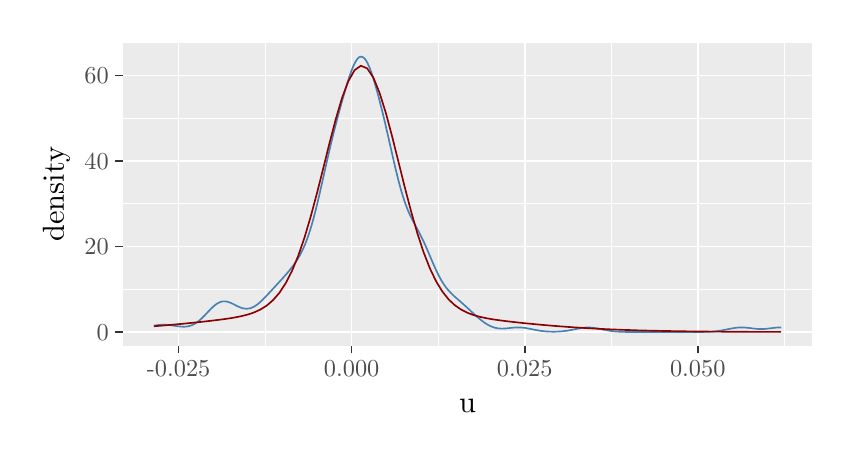
\begin{tikzpicture}[x=1pt,y=1pt]
\definecolor{fillColor}{RGB}{255,255,255}
\path[use as bounding box,fill=fillColor,fill opacity=0.00] (0,0) rectangle (289.08,144.54);
\begin{scope}
\path[clip] (  0.00,  0.00) rectangle (289.08,144.54);
\definecolor{drawColor}{RGB}{255,255,255}
\definecolor{fillColor}{RGB}{255,255,255}

\path[draw=drawColor,line width= 0.6pt,line join=round,line cap=round,fill=fillColor] (  0.00,  0.00) rectangle (289.08,144.54);
\end{scope}
\begin{scope}
\path[clip] ( 34.27, 29.59) rectangle (283.58,139.04);
\definecolor{fillColor}{gray}{0.92}

\path[fill=fillColor] ( 34.27, 29.59) rectangle (283.58,139.04);
\definecolor{drawColor}{RGB}{255,255,255}

\path[draw=drawColor,line width= 0.3pt,line join=round] ( 34.27, 50.02) --
	(283.58, 50.02);

\path[draw=drawColor,line width= 0.3pt,line join=round] ( 34.27, 80.94) --
	(283.58, 80.94);

\path[draw=drawColor,line width= 0.3pt,line join=round] ( 34.27,111.85) --
	(283.58,111.85);

\path[draw=drawColor,line width= 0.3pt,line join=round] ( 85.80, 29.59) --
	( 85.80,139.04);

\path[draw=drawColor,line width= 0.3pt,line join=round] (148.33, 29.59) --
	(148.33,139.04);

\path[draw=drawColor,line width= 0.3pt,line join=round] (210.86, 29.59) --
	(210.86,139.04);

\path[draw=drawColor,line width= 0.3pt,line join=round] (273.40, 29.59) --
	(273.40,139.04);

\path[draw=drawColor,line width= 0.6pt,line join=round] ( 34.27, 34.56) --
	(283.58, 34.56);

\path[draw=drawColor,line width= 0.6pt,line join=round] ( 34.27, 65.48) --
	(283.58, 65.48);

\path[draw=drawColor,line width= 0.6pt,line join=round] ( 34.27, 96.39) --
	(283.58, 96.39);

\path[draw=drawColor,line width= 0.6pt,line join=round] ( 34.27,127.31) --
	(283.58,127.31);

\path[draw=drawColor,line width= 0.6pt,line join=round] ( 54.53, 29.59) --
	( 54.53,139.04);

\path[draw=drawColor,line width= 0.6pt,line join=round] (117.07, 29.59) --
	(117.07,139.04);

\path[draw=drawColor,line width= 0.6pt,line join=round] (179.60, 29.59) --
	(179.60,139.04);

\path[draw=drawColor,line width= 0.6pt,line join=round] (242.13, 29.59) --
	(242.13,139.04);
\definecolor{drawColor}{RGB}{70,130,180}

\path[draw=drawColor,line width= 0.6pt,line join=round] ( 45.60, 36.86) --
	( 46.04, 36.94) --
	( 46.49, 37.01) --
	( 46.93, 37.07) --
	( 47.37, 37.11) --
	( 47.82, 37.15) --
	( 48.26, 37.17) --
	( 48.70, 37.19) --
	( 49.15, 37.19) --
	( 49.59, 37.18) --
	( 50.04, 37.16) --
	( 50.48, 37.13) --
	( 50.92, 37.09) --
	( 51.37, 37.05) --
	( 51.81, 37.00) --
	( 52.25, 36.94) --
	( 52.70, 36.87) --
	( 53.14, 36.81) --
	( 53.58, 36.74) --
	( 54.03, 36.68) --
	( 54.47, 36.62) --
	( 54.91, 36.57) --
	( 55.36, 36.53) --
	( 55.80, 36.50) --
	( 56.25, 36.48) --
	( 56.69, 36.49) --
	( 57.13, 36.51) --
	( 57.58, 36.56) --
	( 58.02, 36.64) --
	( 58.46, 36.74) --
	( 58.91, 36.87) --
	( 59.35, 37.04) --
	( 59.79, 37.24) --
	( 60.24, 37.47) --
	( 60.68, 37.73) --
	( 61.12, 38.02) --
	( 61.57, 38.35) --
	( 62.01, 38.71) --
	( 62.45, 39.09) --
	( 62.90, 39.50) --
	( 63.34, 39.94) --
	( 63.79, 40.38) --
	( 64.23, 40.85) --
	( 64.67, 41.32) --
	( 65.12, 41.79) --
	( 65.56, 42.26) --
	( 66.00, 42.72) --
	( 66.45, 43.16) --
	( 66.89, 43.58) --
	( 67.33, 43.98) --
	( 67.78, 44.35) --
	( 68.22, 44.67) --
	( 68.66, 44.95) --
	( 69.11, 45.18) --
	( 69.55, 45.37) --
	( 69.99, 45.51) --
	( 70.44, 45.61) --
	( 70.88, 45.65) --
	( 71.33, 45.64) --
	( 71.77, 45.59) --
	( 72.21, 45.49) --
	( 72.66, 45.36) --
	( 73.10, 45.20) --
	( 73.54, 45.02) --
	( 73.99, 44.81) --
	( 74.43, 44.59) --
	( 74.87, 44.37) --
	( 75.32, 44.14) --
	( 75.76, 43.92) --
	( 76.20, 43.71) --
	( 76.65, 43.52) --
	( 77.09, 43.35) --
	( 77.53, 43.21) --
	( 77.98, 43.10) --
	( 78.42, 43.03) --
	( 78.87, 42.99) --
	( 79.31, 42.99) --
	( 79.75, 43.03) --
	( 80.20, 43.11) --
	( 80.64, 43.23) --
	( 81.08, 43.40) --
	( 81.53, 43.60) --
	( 81.97, 43.85) --
	( 82.41, 44.12) --
	( 82.86, 44.43) --
	( 83.30, 44.77) --
	( 83.74, 45.15) --
	( 84.19, 45.54) --
	( 84.63, 45.96) --
	( 85.07, 46.39) --
	( 85.52, 46.84) --
	( 85.96, 47.30) --
	( 86.41, 47.77) --
	( 86.85, 48.24) --
	( 87.29, 48.72) --
	( 87.74, 49.20) --
	( 88.18, 49.68) --
	( 88.62, 50.17) --
	( 89.07, 50.65) --
	( 89.51, 51.13) --
	( 89.95, 51.61) --
	( 90.40, 52.09) --
	( 90.84, 52.57) --
	( 91.28, 53.05) --
	( 91.73, 53.54) --
	( 92.17, 54.03) --
	( 92.62, 54.52) --
	( 93.06, 55.02) --
	( 93.50, 55.53) --
	( 93.95, 56.04) --
	( 94.39, 56.57) --
	( 94.83, 57.11) --
	( 95.28, 57.67) --
	( 95.72, 58.25) --
	( 96.16, 58.85) --
	( 96.61, 59.48) --
	( 97.05, 60.14) --
	( 97.49, 60.83) --
	( 97.94, 61.57) --
	( 98.38, 62.35) --
	( 98.82, 63.19) --
	( 99.27, 64.09) --
	( 99.71, 65.05) --
	(100.16, 66.07) --
	(100.60, 67.18) --
	(101.04, 68.35) --
	(101.49, 69.61) --
	(101.93, 70.97) --
	(102.37, 72.40) --
	(102.82, 73.92) --
	(103.26, 75.52) --
	(103.70, 77.19) --
	(104.15, 78.92) --
	(104.59, 80.73) --
	(105.03, 82.60) --
	(105.48, 84.51) --
	(105.92, 86.45) --
	(106.36, 88.42) --
	(106.81, 90.40) --
	(107.25, 92.38) --
	(107.70, 94.36) --
	(108.14, 96.32) --
	(108.58, 98.26) --
	(109.03,100.17) --
	(109.47,102.05) --
	(109.91,103.90) --
	(110.36,105.71) --
	(110.80,107.48) --
	(111.24,109.21) --
	(111.69,110.92) --
	(112.13,112.59) --
	(112.57,114.25) --
	(113.02,115.87) --
	(113.46,117.48) --
	(113.90,119.05) --
	(114.35,120.60) --
	(114.79,122.13) --
	(115.24,123.61) --
	(115.68,125.05) --
	(116.12,126.44) --
	(116.57,127.75) --
	(117.01,128.98) --
	(117.45,130.10) --
	(117.90,131.12) --
	(118.34,132.00) --
	(118.78,132.75) --
	(119.23,133.35) --
	(119.67,133.77) --
	(120.11,134.01) --
	(120.56,134.06) --
	(121.00,133.95) --
	(121.45,133.66) --
	(121.89,133.20) --
	(122.33,132.58) --
	(122.78,131.79) --
	(123.22,130.84) --
	(123.66,129.77) --
	(124.11,128.59) --
	(124.55,127.30) --
	(124.99,125.92) --
	(125.44,124.46) --
	(125.88,122.92) --
	(126.32,121.31) --
	(126.77,119.66) --
	(127.21,117.95) --
	(127.65,116.20) --
	(128.10,114.42) --
	(128.54,112.59) --
	(128.99,110.73) --
	(129.43,108.84) --
	(129.87,106.92) --
	(130.32,104.99) --
	(130.76,103.04) --
	(131.20,101.08) --
	(131.65, 99.13) --
	(132.09, 97.19) --
	(132.53, 95.28) --
	(132.98, 93.40) --
	(133.42, 91.57) --
	(133.86, 89.79) --
	(134.31, 88.08) --
	(134.75, 86.45) --
	(135.19, 84.92) --
	(135.64, 83.46) --
	(136.08, 82.10) --
	(136.53, 80.82) --
	(136.97, 79.63) --
	(137.41, 78.52) --
	(137.86, 77.49) --
	(138.30, 76.53) --
	(138.74, 75.62) --
	(139.19, 74.75) --
	(139.63, 73.91) --
	(140.07, 73.09) --
	(140.52, 72.27) --
	(140.96, 71.45) --
	(141.40, 70.62) --
	(141.85, 69.76) --
	(142.29, 68.88) --
	(142.73, 67.97) --
	(143.18, 67.03) --
	(143.62, 66.06) --
	(144.07, 65.06) --
	(144.51, 64.03) --
	(144.95, 63.00) --
	(145.40, 61.95) --
	(145.84, 60.90) --
	(146.28, 59.86) --
	(146.73, 58.83) --
	(147.17, 57.83) --
	(147.61, 56.86) --
	(148.06, 55.93) --
	(148.50, 55.04) --
	(148.94, 54.20) --
	(149.39, 53.40) --
	(149.83, 52.65) --
	(150.27, 51.96) --
	(150.72, 51.31) --
	(151.16, 50.71) --
	(151.61, 50.15) --
	(152.05, 49.62) --
	(152.49, 49.13) --
	(152.94, 48.66) --
	(153.38, 48.23) --
	(153.82, 47.81) --
	(154.27, 47.40) --
	(154.71, 47.01) --
	(155.15, 46.62) --
	(155.60, 46.23) --
	(156.04, 45.84) --
	(156.48, 45.45) --
	(156.93, 45.06) --
	(157.37, 44.67) --
	(157.82, 44.27) --
	(158.26, 43.87) --
	(158.70, 43.46) --
	(159.15, 43.05) --
	(159.59, 42.64) --
	(160.03, 42.22) --
	(160.48, 41.81) --
	(160.92, 41.40) --
	(161.36, 40.99) --
	(161.81, 40.59) --
	(162.25, 40.20) --
	(162.69, 39.81) --
	(163.14, 39.44) --
	(163.58, 39.07) --
	(164.02, 38.72) --
	(164.47, 38.39) --
	(164.91, 38.06) --
	(165.36, 37.76) --
	(165.80, 37.48) --
	(166.24, 37.22) --
	(166.69, 36.98) --
	(167.13, 36.76) --
	(167.57, 36.56) --
	(168.02, 36.38) --
	(168.46, 36.23) --
	(168.90, 36.11) --
	(169.35, 36.00) --
	(169.79, 35.92) --
	(170.23, 35.86) --
	(170.68, 35.82) --
	(171.12, 35.80) --
	(171.56, 35.80) --
	(172.01, 35.81) --
	(172.45, 35.83) --
	(172.90, 35.87) --
	(173.34, 35.91) --
	(173.78, 35.96) --
	(174.23, 36.01) --
	(174.67, 36.05) --
	(175.11, 36.10) --
	(175.56, 36.14) --
	(176.00, 36.18) --
	(176.44, 36.20) --
	(176.89, 36.22) --
	(177.33, 36.22) --
	(177.77, 36.21) --
	(178.22, 36.19) --
	(178.66, 36.16) --
	(179.10, 36.11) --
	(179.55, 36.06) --
	(179.99, 36.00) --
	(180.44, 35.92) --
	(180.88, 35.84) --
	(181.32, 35.76) --
	(181.77, 35.67) --
	(182.21, 35.58) --
	(182.65, 35.49) --
	(183.10, 35.40) --
	(183.54, 35.31) --
	(183.98, 35.23) --
	(184.43, 35.15) --
	(184.87, 35.08) --
	(185.31, 35.01) --
	(185.76, 34.95) --
	(186.20, 34.89) --
	(186.64, 34.85) --
	(187.09, 34.80) --
	(187.53, 34.77) --
	(187.98, 34.74) --
	(188.42, 34.72) --
	(188.86, 34.70) --
	(189.31, 34.69) --
	(189.75, 34.68) --
	(190.19, 34.68) --
	(190.64, 34.69) --
	(191.08, 34.70) --
	(191.52, 34.71) --
	(191.97, 34.74) --
	(192.41, 34.77) --
	(192.85, 34.80) --
	(193.30, 34.84) --
	(193.74, 34.89) --
	(194.19, 34.94) --
	(194.63, 35.00) --
	(195.07, 35.07) --
	(195.52, 35.14) --
	(195.96, 35.22) --
	(196.40, 35.31) --
	(196.85, 35.39) --
	(197.29, 35.48) --
	(197.73, 35.57) --
	(198.18, 35.66) --
	(198.62, 35.75) --
	(199.06, 35.83) --
	(199.51, 35.91) --
	(199.95, 35.98) --
	(200.39, 36.05) --
	(200.84, 36.10) --
	(201.28, 36.15) --
	(201.73, 36.18) --
	(202.17, 36.19) --
	(202.61, 36.20) --
	(203.06, 36.19) --
	(203.50, 36.16) --
	(203.94, 36.13) --
	(204.39, 36.08) --
	(204.83, 36.02) --
	(205.27, 35.95) --
	(205.72, 35.88) --
	(206.16, 35.80) --
	(206.60, 35.71) --
	(207.05, 35.62) --
	(207.49, 35.53) --
	(207.93, 35.44) --
	(208.38, 35.35) --
	(208.82, 35.27) --
	(209.27, 35.19) --
	(209.71, 35.11) --
	(210.15, 35.04) --
	(210.60, 34.97) --
	(211.04, 34.91) --
	(211.48, 34.86) --
	(211.93, 34.81) --
	(212.37, 34.77) --
	(212.81, 34.74) --
	(213.26, 34.71) --
	(213.70, 34.68) --
	(214.14, 34.66) --
	(214.59, 34.64) --
	(215.03, 34.62) --
	(215.47, 34.61) --
	(215.92, 34.60) --
	(216.36, 34.59) --
	(216.81, 34.58) --
	(217.25, 34.58) --
	(217.69, 34.57) --
	(218.14, 34.57) --
	(218.58, 34.57) --
	(219.02, 34.57) --
	(219.47, 34.57) --
	(219.91, 34.56) --
	(220.35, 34.56) --
	(220.80, 34.56) --
	(221.24, 34.56) --
	(221.68, 34.56) --
	(222.13, 34.56) --
	(222.57, 34.56) --
	(223.02, 34.56) --
	(223.46, 34.56) --
	(223.90, 34.56) --
	(224.35, 34.56) --
	(224.79, 34.56) --
	(225.23, 34.56) --
	(225.68, 34.56) --
	(226.12, 34.56) --
	(226.56, 34.56) --
	(227.01, 34.56) --
	(227.45, 34.56) --
	(227.89, 34.56) --
	(228.34, 34.56) --
	(228.78, 34.56) --
	(229.22, 34.56) --
	(229.67, 34.56) --
	(230.11, 34.56) --
	(230.56, 34.56) --
	(231.00, 34.56) --
	(231.44, 34.56) --
	(231.89, 34.56) --
	(232.33, 34.56) --
	(232.77, 34.56) --
	(233.22, 34.56) --
	(233.66, 34.56) --
	(234.10, 34.56) --
	(234.55, 34.56) --
	(234.99, 34.56) --
	(235.43, 34.56) --
	(235.88, 34.56) --
	(236.32, 34.56) --
	(236.76, 34.56) --
	(237.21, 34.56) --
	(237.65, 34.56) --
	(238.10, 34.56) --
	(238.54, 34.56) --
	(238.98, 34.56) --
	(239.43, 34.56) --
	(239.87, 34.56) --
	(240.31, 34.56) --
	(240.76, 34.57) --
	(241.20, 34.57) --
	(241.64, 34.57) --
	(242.09, 34.57) --
	(242.53, 34.57) --
	(242.97, 34.58) --
	(243.42, 34.58) --
	(243.86, 34.59) --
	(244.30, 34.60) --
	(244.75, 34.61) --
	(245.19, 34.62) --
	(245.64, 34.64) --
	(246.08, 34.65) --
	(246.52, 34.67) --
	(246.97, 34.70) --
	(247.41, 34.73) --
	(247.85, 34.77) --
	(248.30, 34.81) --
	(248.74, 34.85) --
	(249.18, 34.91) --
	(249.63, 34.97) --
	(250.07, 35.03) --
	(250.51, 35.10) --
	(250.96, 35.18) --
	(251.40, 35.26) --
	(251.84, 35.34) --
	(252.29, 35.43) --
	(252.73, 35.52) --
	(253.18, 35.61) --
	(253.62, 35.70) --
	(254.06, 35.79) --
	(254.51, 35.87) --
	(254.95, 35.95) --
	(255.39, 36.02) --
	(255.84, 36.08) --
	(256.28, 36.13) --
	(256.72, 36.17) --
	(257.17, 36.20) --
	(257.61, 36.21) --
	(258.05, 36.22) --
	(258.50, 36.21) --
	(258.94, 36.19) --
	(259.39, 36.16) --
	(259.83, 36.12) --
	(260.27, 36.07) --
	(260.72, 36.02) --
	(261.16, 35.97) --
	(261.60, 35.91) --
	(262.05, 35.85) --
	(262.49, 35.80) --
	(262.93, 35.76) --
	(263.38, 35.71) --
	(263.82, 35.68) --
	(264.26, 35.66) --
	(264.71, 35.65) --
	(265.15, 35.64) --
	(265.59, 35.65) --
	(266.04, 35.67) --
	(266.48, 35.70) --
	(266.93, 35.74) --
	(267.37, 35.78) --
	(267.81, 35.84) --
	(268.26, 35.89) --
	(268.70, 35.95) --
	(269.14, 36.00) --
	(269.59, 36.06) --
	(270.03, 36.10) --
	(270.47, 36.15) --
	(270.92, 36.18) --
	(271.36, 36.20) --
	(271.80, 36.22) --
	(272.25, 36.22);
\definecolor{drawColor}{RGB}{139,0,0}

\path[draw=drawColor,line width= 0.6pt,line join=round] ( 45.60, 36.64) --
	( 47.87, 36.82) --
	( 50.13, 37.01) --
	( 52.40, 37.21) --
	( 54.67, 37.42) --
	( 56.93, 37.63) --
	( 59.20, 37.86) --
	( 61.47, 38.10) --
	( 63.73, 38.34) --
	( 66.00, 38.60) --
	( 68.26, 38.87) --
	( 70.53, 39.16) --
	( 72.80, 39.48) --
	( 75.06, 39.86) --
	( 77.33, 40.32) --
	( 79.60, 40.90) --
	( 81.86, 41.66) --
	( 84.13, 42.71) --
	( 86.40, 44.13) --
	( 88.66, 46.08) --
	( 90.93, 48.69) --
	( 93.20, 52.13) --
	( 95.46, 56.53) --
	( 97.73, 62.01) --
	(100.00, 68.59) --
	(102.26, 76.22) --
	(104.53, 84.70) --
	(106.80, 93.71) --
	(109.06,102.82) --
	(111.33,111.50) --
	(113.59,119.14) --
	(115.86,125.20) --
	(118.13,129.19) --
	(120.39,130.79) --
	(122.66,129.85) --
	(124.93,126.45) --
	(127.19,120.89) --
	(129.46,113.59) --
	(131.73,105.10) --
	(133.99, 96.03) --
	(136.26, 86.90) --
	(138.53, 78.21) --
	(140.79, 70.30) --
	(143.06, 63.40) --
	(145.33, 57.59) --
	(147.59, 52.88) --
	(149.86, 49.17) --
	(152.12, 46.34) --
	(154.39, 44.21) --
	(156.66, 42.65) --
	(158.92, 41.51) --
	(161.19, 40.67) --
	(163.46, 40.04) --
	(165.72, 39.56) --
	(167.99, 39.16) --
	(170.26, 38.83) --
	(172.52, 38.54) --
	(174.79, 38.27) --
	(177.06, 38.02) --
	(179.32, 37.78) --
	(181.59, 37.56) --
	(183.86, 37.34) --
	(186.12, 37.13) --
	(188.39, 36.94) --
	(190.65, 36.75) --
	(192.92, 36.58) --
	(195.19, 36.41) --
	(197.45, 36.25) --
	(199.72, 36.11) --
	(201.99, 35.97) --
	(204.25, 35.84) --
	(206.52, 35.72) --
	(208.79, 35.61) --
	(211.05, 35.51) --
	(213.32, 35.42) --
	(215.59, 35.33) --
	(217.85, 35.26) --
	(220.12, 35.18) --
	(222.39, 35.12) --
	(224.65, 35.06) --
	(226.92, 35.01) --
	(229.18, 34.96) --
	(231.45, 34.92) --
	(233.72, 34.88) --
	(235.98, 34.84) --
	(238.25, 34.81) --
	(240.52, 34.78) --
	(242.78, 34.76) --
	(245.05, 34.73) --
	(247.32, 34.71) --
	(249.58, 34.70) --
	(251.85, 34.68) --
	(254.12, 34.67) --
	(256.38, 34.65) --
	(258.65, 34.64) --
	(260.92, 34.63) --
	(263.18, 34.63) --
	(265.45, 34.62) --
	(267.71, 34.61) --
	(269.98, 34.61) --
	(272.25, 34.60);
\end{scope}
\begin{scope}
\path[clip] (  0.00,  0.00) rectangle (289.08,144.54);
\definecolor{drawColor}{gray}{0.30}

\node[text=drawColor,anchor=base east,inner sep=0pt, outer sep=0pt, scale=  0.88] at ( 29.32, 31.53) {0};

\node[text=drawColor,anchor=base east,inner sep=0pt, outer sep=0pt, scale=  0.88] at ( 29.32, 62.45) {20};

\node[text=drawColor,anchor=base east,inner sep=0pt, outer sep=0pt, scale=  0.88] at ( 29.32, 93.36) {40};

\node[text=drawColor,anchor=base east,inner sep=0pt, outer sep=0pt, scale=  0.88] at ( 29.32,124.28) {60};
\end{scope}
\begin{scope}
\path[clip] (  0.00,  0.00) rectangle (289.08,144.54);
\definecolor{drawColor}{gray}{0.20}

\path[draw=drawColor,line width= 0.6pt,line join=round] ( 31.52, 34.56) --
	( 34.27, 34.56);

\path[draw=drawColor,line width= 0.6pt,line join=round] ( 31.52, 65.48) --
	( 34.27, 65.48);

\path[draw=drawColor,line width= 0.6pt,line join=round] ( 31.52, 96.39) --
	( 34.27, 96.39);

\path[draw=drawColor,line width= 0.6pt,line join=round] ( 31.52,127.31) --
	( 34.27,127.31);
\end{scope}
\begin{scope}
\path[clip] (  0.00,  0.00) rectangle (289.08,144.54);
\definecolor{drawColor}{gray}{0.20}

\path[draw=drawColor,line width= 0.6pt,line join=round] ( 54.53, 26.84) --
	( 54.53, 29.59);

\path[draw=drawColor,line width= 0.6pt,line join=round] (117.07, 26.84) --
	(117.07, 29.59);

\path[draw=drawColor,line width= 0.6pt,line join=round] (179.60, 26.84) --
	(179.60, 29.59);

\path[draw=drawColor,line width= 0.6pt,line join=round] (242.13, 26.84) --
	(242.13, 29.59);
\end{scope}
\begin{scope}
\path[clip] (  0.00,  0.00) rectangle (289.08,144.54);
\definecolor{drawColor}{gray}{0.30}

\node[text=drawColor,anchor=base,inner sep=0pt, outer sep=0pt, scale=  0.88] at ( 54.53, 18.58) {-0.025};

\node[text=drawColor,anchor=base,inner sep=0pt, outer sep=0pt, scale=  0.88] at (117.07, 18.58) {0.000};

\node[text=drawColor,anchor=base,inner sep=0pt, outer sep=0pt, scale=  0.88] at (179.60, 18.58) {0.025};

\node[text=drawColor,anchor=base,inner sep=0pt, outer sep=0pt, scale=  0.88] at (242.13, 18.58) {0.050};
\end{scope}
\begin{scope}
\path[clip] (  0.00,  0.00) rectangle (289.08,144.54);
\definecolor{drawColor}{RGB}{0,0,0}

\node[text=drawColor,anchor=base,inner sep=0pt, outer sep=0pt, scale=  1.10] at (158.92,  5.50) {u};
\end{scope}
\begin{scope}
\path[clip] (  0.00,  0.00) rectangle (289.08,144.54);
\definecolor{drawColor}{RGB}{0,0,0}

\node[text=drawColor,rotate= 90.00,anchor=base,inner sep=0pt, outer sep=0pt, scale=  1.10] at ( 13.08, 84.31) {density};
\end{scope}
\end{tikzpicture}

  \caption{Historical and MJD related Apple stock Log-returns distribution in the risk-averse world}
  \floatfoot{The above blue density curve is constructed over the historical data of the Apple share of stock price evolution from 18th May 2017 to 18th May 2018. while the red curve is constructed from time-series genereated by the function \textit{mjd\_ts} taking the risk-averse parameters \ref{eq:methodology:arg:merton:riskaverse} as arguments.
  }
  \label{p:methodology:density:aapl:merton:riskaverse}
\end{figure}

Consequently, for the purpose of that master thesis, the set \ref{eq:methodology:arg:merton:riskaverse} is the one that will be used together with the function \textit{mjd\_ts()} whenever performing the computation of time series using the MJD model within the real world constraints.











%%%%%%%%%%%%%%%%%%%%%%%%%%%%%%%
%
%
%
% HERE
%
%
%
%%%%%%%%%%%%%%%%%%%%%%%%%%%%%%%%


% SUBSECTION: Heston's model calibration
%%%%%%%%%%%%%%%%%%%%%%%%%%%%%%%%%%%%%%%%%%%%%%%%%%%%%%%%%%%%%%%%%%%%%%%%%%%%%%%%
% Heston
%%%%%%%%%%%%%%%%%%%%%%%%%%%%%%%%%%%%%%%%%%%%%%%%%%%%%%%%%%%%%%%%%%%%%%%%%%%%%%%%
\subsection{Heston's model calibration}
\label{sub:methodology:calibration:heston}

\subsubsection*{Calibration of parameters for option pricing}

In order to use the function \textit{hsv\_call} based on \cref{eq:other:call:heston} to compute the price of European call options on an underlying with increments driven by the HSV model, the parameters $\left\{ V(0), \kappa, \theta, \sigma, \rho \right\}$ must be calibrated with respect to the available market data.
Therefore, the so estimated parameters will be in line with the risk-neutral measure, or more specifically $\kappa$ and $\theta$, which are the only ones needed to be adapted to make \cref{eq:other:hsvvol:riskless} risk-neutral.

To do so and similarly as it was done for the MJD option model, the least-square non-linear analysis will be used together with data on Apple call option as a template.
In that respect, the theoretical models to calibrate are given by \crefrange{eq:other:call:heston}{eq:other:call:heston:pi2} along with \cref{eq:other:heston:psi}, implemented by the R function \textit{hsv\_call}.

Moreover, to stay in a range of acceptable values, the parameters of the HSV model should lie between some defined boundaries. 

De facto, the mean-reversion speed ($\kappa$), the long-run variance ($\theta$) and the volatility of the volatility ($\sigma$) need to take values that together respect the Feller's condition (see \cref{sub:other:heston:feller}). 
Additionally, $\sigma$ must range between 0 and 1 and, according to \citet{cristo2015} $\kappa$ should be positive to avoid mean aversion.
Although the correlation coefficient $\rho$ may take any value from $[-1, 1]$, typically the correlation between the stock price increments and their intrinsic volatility is negative. Consequently, the boundaries of $\rho$ are set as $]0, -1[$.

According to those constraints and due to the presence of multiple local minima, the \textit{lsqnonlin} function returns the \cref{t:methodology:call:heston:estimate1} as the whole sets of parameters that make the function \textit{hsv\_call} better fit with reality.

\begin{table}[ht]
\centering
\begin{tabular}{rrrrr}
  \hline
v0 & theta & sigma & rho & kappa \\ 
  \hline
  0.03851 & 0.05142 & 0.29539 & -0.49338 & 1.99931 \\ 
  0.03774 & 0.04832 & 0.30687 & -0.40213 & 3.00036 \\ 
  0.03910 & 0.04948 & 0.40736 & -0.50193 & 3.00005 \\ 
  0.03798 & 0.04872 & 0.50379 & -0.39878 & 4.00106 \\
  0.03740 & 0.04754 & 0.30583 & -0.60126 & 4.00096 \\ 
  0.03661 & 0.04604 & 0.30659 & -0.40295 & 5.00152 \\ 
  0.03921 & 0.04709 & 0.50753 & -0.50170 & 5.00152 \\ 
   \hline
\end{tabular}
\caption{Best estimates for HSV call option model} 
\label{t:methodology:call:heston:estimate1}
\end{table}

However, the set of arguments \ref{eq:methodology:arg:heston:riskneutral} is the one making respond the model the best with what is observed in reality.
Indeed when passing that set to the R function \textit{call\_heston}, for all strikes and maturities from \cref{t:methodology:strike,t:methodology:maturity}  more than $70\%$ of the so generated prices are within the bid-ask spread of the historical data.

\begin{align}
  \left \{
  \begin{array}{lcl}
    V(0) &= &0.03798218, \\
    \theta &= &0.04871543, \\
    \sigma &= &0.50378803, \\
    \rho &= &-0.39877827, \\
    \kappa &= &4.00105546 
  \end{array}
  \right \}  
  \label{eq:methodology:arg:heston:riskneutral}
\end{align}

\Cref{p:methodology:impliedvol:aapl:heston} confronts the blue colored volatility smiles computed from market data, with those dotted in red, calculated from data provided by the function \textit{hsv\_call} which takes the items of the set \ref{eq:methodology:arg:heston:riskneutral} as parameters.

\begin{figure}[ht]
  \centering
  % Created by tikzDevice version 0.11 on 2018-07-20 21:55:59
% !TEX encoding = UTF-8 Unicode
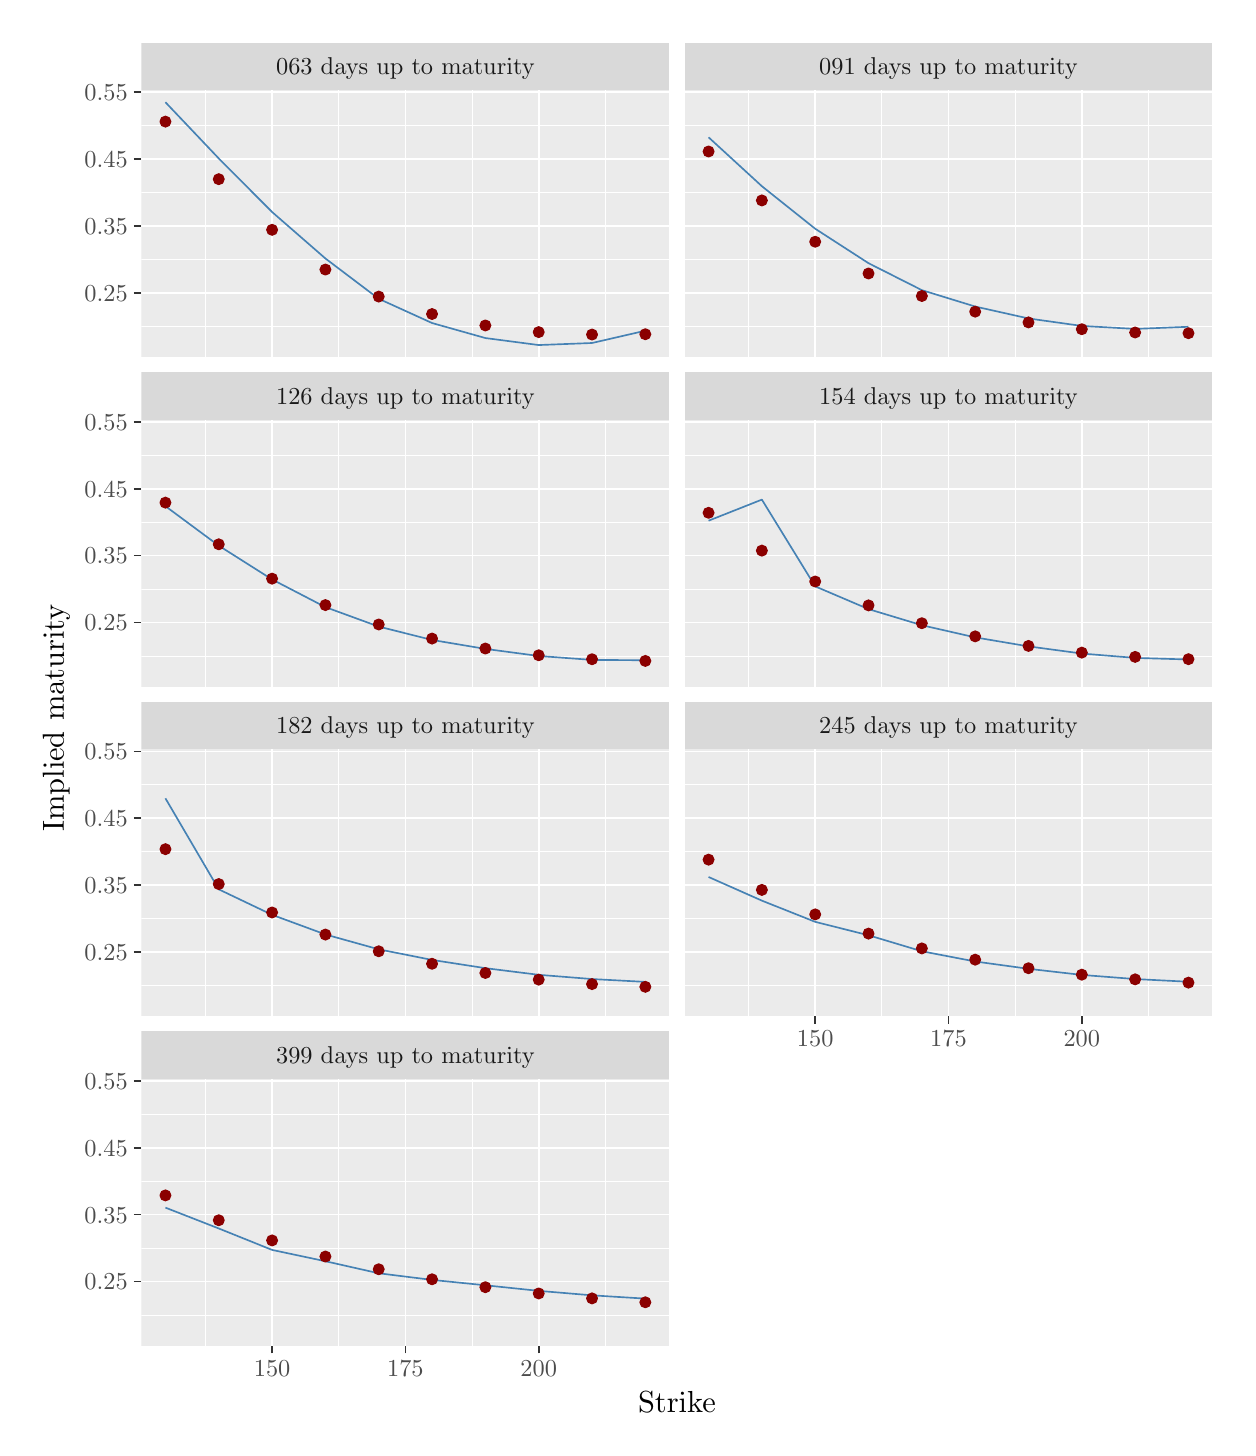
\begin{tikzpicture}[x=1pt,y=1pt]
\definecolor{fillColor}{RGB}{255,255,255}
\path[use as bounding box,fill=fillColor,fill opacity=0.00] (0,0) rectangle (433.62,505.89);
\begin{scope}
\path[clip] (  0.00,  0.00) rectangle (433.62,505.89);
\definecolor{drawColor}{RGB}{255,255,255}
\definecolor{fillColor}{RGB}{255,255,255}

\path[draw=drawColor,line width= 0.6pt,line join=round,line cap=round,fill=fillColor] (  0.00,  0.00) rectangle (433.62,505.89);
\end{scope}
\begin{scope}
\path[clip] ( 41.11,386.81) rectangle (231.87,483.33);
\definecolor{fillColor}{gray}{0.92}

\path[fill=fillColor] ( 41.11,386.81) rectangle (231.87,483.33);
\definecolor{drawColor}{RGB}{255,255,255}

\path[draw=drawColor,line width= 0.3pt,line join=round] ( 41.11,397.93) --
	(231.87,397.93);

\path[draw=drawColor,line width= 0.3pt,line join=round] ( 41.11,422.11) --
	(231.87,422.11);

\path[draw=drawColor,line width= 0.3pt,line join=round] ( 41.11,446.28) --
	(231.87,446.28);

\path[draw=drawColor,line width= 0.3pt,line join=round] ( 41.11,470.45) --
	(231.87,470.45);

\path[draw=drawColor,line width= 0.3pt,line join=round] ( 64.23,386.81) --
	( 64.23,483.33);

\path[draw=drawColor,line width= 0.3pt,line join=round] (112.40,386.81) --
	(112.40,483.33);

\path[draw=drawColor,line width= 0.3pt,line join=round] (160.57,386.81) --
	(160.57,483.33);

\path[draw=drawColor,line width= 0.3pt,line join=round] (208.74,386.81) --
	(208.74,483.33);

\path[draw=drawColor,line width= 0.6pt,line join=round] ( 41.11,410.02) --
	(231.87,410.02);

\path[draw=drawColor,line width= 0.6pt,line join=round] ( 41.11,434.19) --
	(231.87,434.19);

\path[draw=drawColor,line width= 0.6pt,line join=round] ( 41.11,458.37) --
	(231.87,458.37);

\path[draw=drawColor,line width= 0.6pt,line join=round] ( 41.11,482.54) --
	(231.87,482.54);

\path[draw=drawColor,line width= 0.6pt,line join=round] ( 88.32,386.81) --
	( 88.32,483.33);

\path[draw=drawColor,line width= 0.6pt,line join=round] (136.49,386.81) --
	(136.49,483.33);

\path[draw=drawColor,line width= 0.6pt,line join=round] (184.66,386.81) --
	(184.66,483.33);
\definecolor{drawColor}{RGB}{70,130,180}

\path[draw=drawColor,line width= 0.6pt,line join=round] ( 49.78,478.94) --
	( 69.05,458.63) --
	( 88.32,439.27) --
	(107.59,422.48) --
	(126.85,407.92) --
	(146.12,399.16) --
	(165.39,393.73) --
	(184.66,391.20) --
	(203.93,391.94) --
	(223.19,396.38);
\definecolor{drawColor}{RGB}{139,0,0}
\definecolor{fillColor}{RGB}{139,0,0}

\path[draw=drawColor,line width= 0.4pt,line join=round,line cap=round,fill=fillColor] ( 49.78,471.94) circle (  1.96);

\path[draw=drawColor,line width= 0.4pt,line join=round,line cap=round,fill=fillColor] ( 69.05,451.14) circle (  1.96);

\path[draw=drawColor,line width= 0.4pt,line join=round,line cap=round,fill=fillColor] ( 88.32,432.84) circle (  1.96);

\path[draw=drawColor,line width= 0.4pt,line join=round,line cap=round,fill=fillColor] (107.59,418.48) circle (  1.96);

\path[draw=drawColor,line width= 0.4pt,line join=round,line cap=round,fill=fillColor] (126.85,408.72) circle (  1.96);

\path[draw=drawColor,line width= 0.4pt,line join=round,line cap=round,fill=fillColor] (146.12,402.41) circle (  1.96);

\path[draw=drawColor,line width= 0.4pt,line join=round,line cap=round,fill=fillColor] (165.39,398.28) circle (  1.96);

\path[draw=drawColor,line width= 0.4pt,line join=round,line cap=round,fill=fillColor] (184.66,395.88) circle (  1.96);

\path[draw=drawColor,line width= 0.4pt,line join=round,line cap=round,fill=fillColor] (203.93,394.99) circle (  1.96);

\path[draw=drawColor,line width= 0.4pt,line join=round,line cap=round,fill=fillColor] (223.19,395.11) circle (  1.96);
\end{scope}
\begin{scope}
\path[clip] ( 41.11,267.74) rectangle (231.87,364.25);
\definecolor{fillColor}{gray}{0.92}

\path[fill=fillColor] ( 41.11,267.74) rectangle (231.87,364.25);
\definecolor{drawColor}{RGB}{255,255,255}

\path[draw=drawColor,line width= 0.3pt,line join=round] ( 41.11,278.86) --
	(231.87,278.86);

\path[draw=drawColor,line width= 0.3pt,line join=round] ( 41.11,303.03) --
	(231.87,303.03);

\path[draw=drawColor,line width= 0.3pt,line join=round] ( 41.11,327.20) --
	(231.87,327.20);

\path[draw=drawColor,line width= 0.3pt,line join=round] ( 41.11,351.38) --
	(231.87,351.38);

\path[draw=drawColor,line width= 0.3pt,line join=round] ( 64.23,267.74) --
	( 64.23,364.25);

\path[draw=drawColor,line width= 0.3pt,line join=round] (112.40,267.74) --
	(112.40,364.25);

\path[draw=drawColor,line width= 0.3pt,line join=round] (160.57,267.74) --
	(160.57,364.25);

\path[draw=drawColor,line width= 0.3pt,line join=round] (208.74,267.74) --
	(208.74,364.25);

\path[draw=drawColor,line width= 0.6pt,line join=round] ( 41.11,290.95) --
	(231.87,290.95);

\path[draw=drawColor,line width= 0.6pt,line join=round] ( 41.11,315.12) --
	(231.87,315.12);

\path[draw=drawColor,line width= 0.6pt,line join=round] ( 41.11,339.29) --
	(231.87,339.29);

\path[draw=drawColor,line width= 0.6pt,line join=round] ( 41.11,363.46) --
	(231.87,363.46);

\path[draw=drawColor,line width= 0.6pt,line join=round] ( 88.32,267.74) --
	( 88.32,364.25);

\path[draw=drawColor,line width= 0.6pt,line join=round] (136.49,267.74) --
	(136.49,364.25);

\path[draw=drawColor,line width= 0.6pt,line join=round] (184.66,267.74) --
	(184.66,364.25);
\definecolor{drawColor}{RGB}{70,130,180}

\path[draw=drawColor,line width= 0.6pt,line join=round] ( 49.78,332.98) --
	( 69.05,318.71) --
	( 88.32,306.50) --
	(107.59,296.51) --
	(126.85,289.47) --
	(146.12,284.64) --
	(165.39,281.41) --
	(184.66,278.85) --
	(203.93,277.43) --
	(223.19,277.30);
\definecolor{drawColor}{RGB}{139,0,0}
\definecolor{fillColor}{RGB}{139,0,0}

\path[draw=drawColor,line width= 0.4pt,line join=round,line cap=round,fill=fillColor] ( 49.78,334.26) circle (  1.96);

\path[draw=drawColor,line width= 0.4pt,line join=round,line cap=round,fill=fillColor] ( 69.05,319.20) circle (  1.96);

\path[draw=drawColor,line width= 0.4pt,line join=round,line cap=round,fill=fillColor] ( 88.32,306.79) circle (  1.96);

\path[draw=drawColor,line width= 0.4pt,line join=round,line cap=round,fill=fillColor] (107.59,297.24) circle (  1.96);

\path[draw=drawColor,line width= 0.4pt,line join=round,line cap=round,fill=fillColor] (126.85,290.23) circle (  1.96);

\path[draw=drawColor,line width= 0.4pt,line join=round,line cap=round,fill=fillColor] (146.12,285.14) circle (  1.96);

\path[draw=drawColor,line width= 0.4pt,line join=round,line cap=round,fill=fillColor] (165.39,281.54) circle (  1.96);

\path[draw=drawColor,line width= 0.4pt,line join=round,line cap=round,fill=fillColor] (184.66,279.10) circle (  1.96);

\path[draw=drawColor,line width= 0.4pt,line join=round,line cap=round,fill=fillColor] (203.93,277.67) circle (  1.96);

\path[draw=drawColor,line width= 0.4pt,line join=round,line cap=round,fill=fillColor] (223.19,277.06) circle (  1.96);
\end{scope}
\begin{scope}
\path[clip] ( 41.11,148.66) rectangle (231.87,245.18);
\definecolor{fillColor}{gray}{0.92}

\path[fill=fillColor] ( 41.11,148.66) rectangle (231.87,245.18);
\definecolor{drawColor}{RGB}{255,255,255}

\path[draw=drawColor,line width= 0.3pt,line join=round] ( 41.11,159.78) --
	(231.87,159.78);

\path[draw=drawColor,line width= 0.3pt,line join=round] ( 41.11,183.96) --
	(231.87,183.96);

\path[draw=drawColor,line width= 0.3pt,line join=round] ( 41.11,208.13) --
	(231.87,208.13);

\path[draw=drawColor,line width= 0.3pt,line join=round] ( 41.11,232.30) --
	(231.87,232.30);

\path[draw=drawColor,line width= 0.3pt,line join=round] ( 64.23,148.66) --
	( 64.23,245.18);

\path[draw=drawColor,line width= 0.3pt,line join=round] (112.40,148.66) --
	(112.40,245.18);

\path[draw=drawColor,line width= 0.3pt,line join=round] (160.57,148.66) --
	(160.57,245.18);

\path[draw=drawColor,line width= 0.3pt,line join=round] (208.74,148.66) --
	(208.74,245.18);

\path[draw=drawColor,line width= 0.6pt,line join=round] ( 41.11,171.87) --
	(231.87,171.87);

\path[draw=drawColor,line width= 0.6pt,line join=round] ( 41.11,196.04) --
	(231.87,196.04);

\path[draw=drawColor,line width= 0.6pt,line join=round] ( 41.11,220.21) --
	(231.87,220.21);

\path[draw=drawColor,line width= 0.6pt,line join=round] ( 41.11,244.39) --
	(231.87,244.39);

\path[draw=drawColor,line width= 0.6pt,line join=round] ( 88.32,148.66) --
	( 88.32,245.18);

\path[draw=drawColor,line width= 0.6pt,line join=round] (136.49,148.66) --
	(136.49,245.18);

\path[draw=drawColor,line width= 0.6pt,line join=round] (184.66,148.66) --
	(184.66,245.18);
\definecolor{drawColor}{RGB}{70,130,180}

\path[draw=drawColor,line width= 0.6pt,line join=round] ( 49.78,227.41) --
	( 69.05,194.52) --
	( 88.32,185.32) --
	(107.59,178.22) --
	(126.85,172.85) --
	(146.12,169.02) --
	(165.39,166.04) --
	(184.66,163.64) --
	(203.93,162.11) --
	(223.19,161.08);
\definecolor{drawColor}{RGB}{139,0,0}
\definecolor{fillColor}{RGB}{139,0,0}

\path[draw=drawColor,line width= 0.4pt,line join=round,line cap=round,fill=fillColor] ( 49.78,209.04) circle (  1.96);

\path[draw=drawColor,line width= 0.4pt,line join=round,line cap=round,fill=fillColor] ( 69.05,196.43) circle (  1.96);

\path[draw=drawColor,line width= 0.4pt,line join=round,line cap=round,fill=fillColor] ( 88.32,186.16) circle (  1.96);

\path[draw=drawColor,line width= 0.4pt,line join=round,line cap=round,fill=fillColor] (107.59,178.18) circle (  1.96);

\path[draw=drawColor,line width= 0.4pt,line join=round,line cap=round,fill=fillColor] (126.85,172.14) circle (  1.96);

\path[draw=drawColor,line width= 0.4pt,line join=round,line cap=round,fill=fillColor] (146.12,167.63) circle (  1.96);

\path[draw=drawColor,line width= 0.4pt,line join=round,line cap=round,fill=fillColor] (165.39,164.30) circle (  1.96);

\path[draw=drawColor,line width= 0.4pt,line join=round,line cap=round,fill=fillColor] (184.66,161.90) circle (  1.96);

\path[draw=drawColor,line width= 0.4pt,line join=round,line cap=round,fill=fillColor] (203.93,160.28) circle (  1.96);

\path[draw=drawColor,line width= 0.4pt,line join=round,line cap=round,fill=fillColor] (223.19,159.30) circle (  1.96);
\end{scope}
\begin{scope}
\path[clip] ( 41.11, 29.59) rectangle (231.87,126.10);
\definecolor{fillColor}{gray}{0.92}

\path[fill=fillColor] ( 41.11, 29.59) rectangle (231.87,126.10);
\definecolor{drawColor}{RGB}{255,255,255}

\path[draw=drawColor,line width= 0.3pt,line join=round] ( 41.11, 40.71) --
	(231.87, 40.71);

\path[draw=drawColor,line width= 0.3pt,line join=round] ( 41.11, 64.88) --
	(231.87, 64.88);

\path[draw=drawColor,line width= 0.3pt,line join=round] ( 41.11, 89.05) --
	(231.87, 89.05);

\path[draw=drawColor,line width= 0.3pt,line join=round] ( 41.11,113.22) --
	(231.87,113.22);

\path[draw=drawColor,line width= 0.3pt,line join=round] ( 64.23, 29.59) --
	( 64.23,126.10);

\path[draw=drawColor,line width= 0.3pt,line join=round] (112.40, 29.59) --
	(112.40,126.10);

\path[draw=drawColor,line width= 0.3pt,line join=round] (160.57, 29.59) --
	(160.57,126.10);

\path[draw=drawColor,line width= 0.3pt,line join=round] (208.74, 29.59) --
	(208.74,126.10);

\path[draw=drawColor,line width= 0.6pt,line join=round] ( 41.11, 52.79) --
	(231.87, 52.79);

\path[draw=drawColor,line width= 0.6pt,line join=round] ( 41.11, 76.97) --
	(231.87, 76.97);

\path[draw=drawColor,line width= 0.6pt,line join=round] ( 41.11,101.14) --
	(231.87,101.14);

\path[draw=drawColor,line width= 0.6pt,line join=round] ( 41.11,125.31) --
	(231.87,125.31);

\path[draw=drawColor,line width= 0.6pt,line join=round] ( 88.32, 29.59) --
	( 88.32,126.10);

\path[draw=drawColor,line width= 0.6pt,line join=round] (136.49, 29.59) --
	(136.49,126.10);

\path[draw=drawColor,line width= 0.6pt,line join=round] (184.66, 29.59) --
	(184.66,126.10);
\definecolor{drawColor}{RGB}{70,130,180}

\path[draw=drawColor,line width= 0.6pt,line join=round] ( 49.78, 79.51) --
	( 69.05, 71.98) --
	( 88.32, 64.23) --
	(107.59, 60.14) --
	(126.85, 55.79) --
	(146.12, 53.40) --
	(165.39, 51.45) --
	(184.66, 49.44) --
	(203.93, 47.82) --
	(223.19, 46.63);
\definecolor{drawColor}{RGB}{139,0,0}
\definecolor{fillColor}{RGB}{139,0,0}

\path[draw=drawColor,line width= 0.4pt,line join=round,line cap=round,fill=fillColor] ( 49.78, 83.93) circle (  1.96);

\path[draw=drawColor,line width= 0.4pt,line join=round,line cap=round,fill=fillColor] ( 69.05, 74.95) circle (  1.96);

\path[draw=drawColor,line width= 0.4pt,line join=round,line cap=round,fill=fillColor] ( 88.32, 67.66) circle (  1.96);

\path[draw=drawColor,line width= 0.4pt,line join=round,line cap=round,fill=fillColor] (107.59, 61.84) circle (  1.96);

\path[draw=drawColor,line width= 0.4pt,line join=round,line cap=round,fill=fillColor] (126.85, 57.24) circle (  1.96);

\path[draw=drawColor,line width= 0.4pt,line join=round,line cap=round,fill=fillColor] (146.12, 53.62) circle (  1.96);

\path[draw=drawColor,line width= 0.4pt,line join=round,line cap=round,fill=fillColor] (165.39, 50.76) circle (  1.96);

\path[draw=drawColor,line width= 0.4pt,line join=round,line cap=round,fill=fillColor] (184.66, 48.50) circle (  1.96);

\path[draw=drawColor,line width= 0.4pt,line join=round,line cap=round,fill=fillColor] (203.93, 46.72) circle (  1.96);

\path[draw=drawColor,line width= 0.4pt,line join=round,line cap=round,fill=fillColor] (223.19, 45.31) circle (  1.96);
\end{scope}
\begin{scope}
\path[clip] (237.37,386.81) rectangle (428.12,483.33);
\definecolor{fillColor}{gray}{0.92}

\path[fill=fillColor] (237.37,386.81) rectangle (428.12,483.33);
\definecolor{drawColor}{RGB}{255,255,255}

\path[draw=drawColor,line width= 0.3pt,line join=round] (237.37,397.93) --
	(428.12,397.93);

\path[draw=drawColor,line width= 0.3pt,line join=round] (237.37,422.11) --
	(428.12,422.11);

\path[draw=drawColor,line width= 0.3pt,line join=round] (237.37,446.28) --
	(428.12,446.28);

\path[draw=drawColor,line width= 0.3pt,line join=round] (237.37,470.45) --
	(428.12,470.45);

\path[draw=drawColor,line width= 0.3pt,line join=round] (260.49,386.81) --
	(260.49,483.33);

\path[draw=drawColor,line width= 0.3pt,line join=round] (308.66,386.81) --
	(308.66,483.33);

\path[draw=drawColor,line width= 0.3pt,line join=round] (356.83,386.81) --
	(356.83,483.33);

\path[draw=drawColor,line width= 0.3pt,line join=round] (405.00,386.81) --
	(405.00,483.33);

\path[draw=drawColor,line width= 0.6pt,line join=round] (237.37,410.02) --
	(428.12,410.02);

\path[draw=drawColor,line width= 0.6pt,line join=round] (237.37,434.19) --
	(428.12,434.19);

\path[draw=drawColor,line width= 0.6pt,line join=round] (237.37,458.37) --
	(428.12,458.37);

\path[draw=drawColor,line width= 0.6pt,line join=round] (237.37,482.54) --
	(428.12,482.54);

\path[draw=drawColor,line width= 0.6pt,line join=round] (284.57,386.81) --
	(284.57,483.33);

\path[draw=drawColor,line width= 0.6pt,line join=round] (332.74,386.81) --
	(332.74,483.33);

\path[draw=drawColor,line width= 0.6pt,line join=round] (380.91,386.81) --
	(380.91,483.33);
\definecolor{drawColor}{RGB}{70,130,180}

\path[draw=drawColor,line width= 0.6pt,line join=round] (246.04,466.27) --
	(265.30,448.60) --
	(284.57,433.23) --
	(303.84,420.78) --
	(323.11,411.04) --
	(342.38,405.12) --
	(361.64,400.81) --
	(380.91,398.11) --
	(400.18,397.03) --
	(419.45,397.80);
\definecolor{drawColor}{RGB}{139,0,0}
\definecolor{fillColor}{RGB}{139,0,0}

\path[draw=drawColor,line width= 0.4pt,line join=round,line cap=round,fill=fillColor] (246.04,461.14) circle (  1.96);

\path[draw=drawColor,line width= 0.4pt,line join=round,line cap=round,fill=fillColor] (265.30,443.46) circle (  1.96);

\path[draw=drawColor,line width= 0.4pt,line join=round,line cap=round,fill=fillColor] (284.57,428.53) circle (  1.96);

\path[draw=drawColor,line width= 0.4pt,line join=round,line cap=round,fill=fillColor] (303.84,417.06) circle (  1.96);

\path[draw=drawColor,line width= 0.4pt,line join=round,line cap=round,fill=fillColor] (323.11,408.92) circle (  1.96);

\path[draw=drawColor,line width= 0.4pt,line join=round,line cap=round,fill=fillColor] (342.38,403.27) circle (  1.96);

\path[draw=drawColor,line width= 0.4pt,line join=round,line cap=round,fill=fillColor] (361.64,399.38) circle (  1.96);

\path[draw=drawColor,line width= 0.4pt,line join=round,line cap=round,fill=fillColor] (380.91,396.93) circle (  1.96);

\path[draw=drawColor,line width= 0.4pt,line join=round,line cap=round,fill=fillColor] (400.18,395.74) circle (  1.96);

\path[draw=drawColor,line width= 0.4pt,line join=round,line cap=round,fill=fillColor] (419.45,395.48) circle (  1.96);
\end{scope}
\begin{scope}
\path[clip] (237.37,267.74) rectangle (428.12,364.25);
\definecolor{fillColor}{gray}{0.92}

\path[fill=fillColor] (237.37,267.74) rectangle (428.12,364.25);
\definecolor{drawColor}{RGB}{255,255,255}

\path[draw=drawColor,line width= 0.3pt,line join=round] (237.37,278.86) --
	(428.12,278.86);

\path[draw=drawColor,line width= 0.3pt,line join=round] (237.37,303.03) --
	(428.12,303.03);

\path[draw=drawColor,line width= 0.3pt,line join=round] (237.37,327.20) --
	(428.12,327.20);

\path[draw=drawColor,line width= 0.3pt,line join=round] (237.37,351.38) --
	(428.12,351.38);

\path[draw=drawColor,line width= 0.3pt,line join=round] (260.49,267.74) --
	(260.49,364.25);

\path[draw=drawColor,line width= 0.3pt,line join=round] (308.66,267.74) --
	(308.66,364.25);

\path[draw=drawColor,line width= 0.3pt,line join=round] (356.83,267.74) --
	(356.83,364.25);

\path[draw=drawColor,line width= 0.3pt,line join=round] (405.00,267.74) --
	(405.00,364.25);

\path[draw=drawColor,line width= 0.6pt,line join=round] (237.37,290.95) --
	(428.12,290.95);

\path[draw=drawColor,line width= 0.6pt,line join=round] (237.37,315.12) --
	(428.12,315.12);

\path[draw=drawColor,line width= 0.6pt,line join=round] (237.37,339.29) --
	(428.12,339.29);

\path[draw=drawColor,line width= 0.6pt,line join=round] (237.37,363.46) --
	(428.12,363.46);

\path[draw=drawColor,line width= 0.6pt,line join=round] (284.57,267.74) --
	(284.57,364.25);

\path[draw=drawColor,line width= 0.6pt,line join=round] (332.74,267.74) --
	(332.74,364.25);

\path[draw=drawColor,line width= 0.6pt,line join=round] (380.91,267.74) --
	(380.91,364.25);
\definecolor{drawColor}{RGB}{70,130,180}

\path[draw=drawColor,line width= 0.6pt,line join=round] (246.04,327.73) --
	(265.30,335.35) --
	(284.57,304.00) --
	(303.84,295.78) --
	(323.11,289.96) --
	(342.38,285.57) --
	(361.64,282.32) --
	(380.91,279.73) --
	(400.18,278.15) --
	(419.45,277.58);
\definecolor{drawColor}{RGB}{139,0,0}
\definecolor{fillColor}{RGB}{139,0,0}

\path[draw=drawColor,line width= 0.4pt,line join=round,line cap=round,fill=fillColor] (246.04,330.58) circle (  1.96);

\path[draw=drawColor,line width= 0.4pt,line join=round,line cap=round,fill=fillColor] (265.30,316.92) circle (  1.96);

\path[draw=drawColor,line width= 0.4pt,line join=round,line cap=round,fill=fillColor] (284.57,305.76) circle (  1.96);

\path[draw=drawColor,line width= 0.4pt,line join=round,line cap=round,fill=fillColor] (303.84,297.13) circle (  1.96);

\path[draw=drawColor,line width= 0.4pt,line join=round,line cap=round,fill=fillColor] (323.11,290.69) circle (  1.96);

\path[draw=drawColor,line width= 0.4pt,line join=round,line cap=round,fill=fillColor] (342.38,285.94) circle (  1.96);

\path[draw=drawColor,line width= 0.4pt,line join=round,line cap=round,fill=fillColor] (361.64,282.48) circle (  1.96);

\path[draw=drawColor,line width= 0.4pt,line join=round,line cap=round,fill=fillColor] (380.91,280.06) circle (  1.96);

\path[draw=drawColor,line width= 0.4pt,line join=round,line cap=round,fill=fillColor] (400.18,278.52) circle (  1.96);

\path[draw=drawColor,line width= 0.4pt,line join=round,line cap=round,fill=fillColor] (419.45,277.69) circle (  1.96);
\end{scope}
\begin{scope}
\path[clip] (237.37,148.66) rectangle (428.12,245.18);
\definecolor{fillColor}{gray}{0.92}

\path[fill=fillColor] (237.37,148.66) rectangle (428.12,245.18);
\definecolor{drawColor}{RGB}{255,255,255}

\path[draw=drawColor,line width= 0.3pt,line join=round] (237.37,159.78) --
	(428.12,159.78);

\path[draw=drawColor,line width= 0.3pt,line join=round] (237.37,183.96) --
	(428.12,183.96);

\path[draw=drawColor,line width= 0.3pt,line join=round] (237.37,208.13) --
	(428.12,208.13);

\path[draw=drawColor,line width= 0.3pt,line join=round] (237.37,232.30) --
	(428.12,232.30);

\path[draw=drawColor,line width= 0.3pt,line join=round] (260.49,148.66) --
	(260.49,245.18);

\path[draw=drawColor,line width= 0.3pt,line join=round] (308.66,148.66) --
	(308.66,245.18);

\path[draw=drawColor,line width= 0.3pt,line join=round] (356.83,148.66) --
	(356.83,245.18);

\path[draw=drawColor,line width= 0.3pt,line join=round] (405.00,148.66) --
	(405.00,245.18);

\path[draw=drawColor,line width= 0.6pt,line join=round] (237.37,171.87) --
	(428.12,171.87);

\path[draw=drawColor,line width= 0.6pt,line join=round] (237.37,196.04) --
	(428.12,196.04);

\path[draw=drawColor,line width= 0.6pt,line join=round] (237.37,220.21) --
	(428.12,220.21);

\path[draw=drawColor,line width= 0.6pt,line join=round] (237.37,244.39) --
	(428.12,244.39);

\path[draw=drawColor,line width= 0.6pt,line join=round] (284.57,148.66) --
	(284.57,245.18);

\path[draw=drawColor,line width= 0.6pt,line join=round] (332.74,148.66) --
	(332.74,245.18);

\path[draw=drawColor,line width= 0.6pt,line join=round] (380.91,148.66) --
	(380.91,245.18);
\definecolor{drawColor}{RGB}{70,130,180}

\path[draw=drawColor,line width= 0.6pt,line join=round] (246.04,198.99) --
	(265.30,190.44) --
	(284.57,182.78) --
	(303.84,177.93) --
	(323.11,172.15) --
	(342.38,168.45) --
	(361.64,165.81) --
	(380.91,163.60) --
	(400.18,162.11) --
	(419.45,161.13);
\definecolor{drawColor}{RGB}{139,0,0}
\definecolor{fillColor}{RGB}{139,0,0}

\path[draw=drawColor,line width= 0.4pt,line join=round,line cap=round,fill=fillColor] (246.04,205.25) circle (  1.96);

\path[draw=drawColor,line width= 0.4pt,line join=round,line cap=round,fill=fillColor] (265.30,194.32) circle (  1.96);

\path[draw=drawColor,line width= 0.4pt,line join=round,line cap=round,fill=fillColor] (284.57,185.47) circle (  1.96);

\path[draw=drawColor,line width= 0.4pt,line join=round,line cap=round,fill=fillColor] (303.84,178.53) circle (  1.96);

\path[draw=drawColor,line width= 0.4pt,line join=round,line cap=round,fill=fillColor] (323.11,173.18) circle (  1.96);

\path[draw=drawColor,line width= 0.4pt,line join=round,line cap=round,fill=fillColor] (342.38,169.11) circle (  1.96);

\path[draw=drawColor,line width= 0.4pt,line join=round,line cap=round,fill=fillColor] (361.64,166.02) circle (  1.96);

\path[draw=drawColor,line width= 0.4pt,line join=round,line cap=round,fill=fillColor] (380.91,163.69) circle (  1.96);

\path[draw=drawColor,line width= 0.4pt,line join=round,line cap=round,fill=fillColor] (400.18,162.00) circle (  1.96);

\path[draw=drawColor,line width= 0.4pt,line join=round,line cap=round,fill=fillColor] (419.45,160.81) circle (  1.96);
\end{scope}
\begin{scope}
\path[clip] ( 41.11,126.10) rectangle (231.87,143.16);
\definecolor{fillColor}{gray}{0.85}

\path[fill=fillColor] ( 41.11,126.10) rectangle (231.87,143.16);
\definecolor{drawColor}{gray}{0.10}

\node[text=drawColor,anchor=base,inner sep=0pt, outer sep=0pt, scale=  0.88] at (136.49,131.60) {399 days up to maturity};
\end{scope}
\begin{scope}
\path[clip] ( 41.11,245.18) rectangle (231.87,262.24);
\definecolor{fillColor}{gray}{0.85}

\path[fill=fillColor] ( 41.11,245.18) rectangle (231.87,262.24);
\definecolor{drawColor}{gray}{0.10}

\node[text=drawColor,anchor=base,inner sep=0pt, outer sep=0pt, scale=  0.88] at (136.49,250.68) {182 days up to maturity};
\end{scope}
\begin{scope}
\path[clip] (237.37,245.18) rectangle (428.12,262.24);
\definecolor{fillColor}{gray}{0.85}

\path[fill=fillColor] (237.37,245.18) rectangle (428.12,262.24);
\definecolor{drawColor}{gray}{0.10}

\node[text=drawColor,anchor=base,inner sep=0pt, outer sep=0pt, scale=  0.88] at (332.74,250.68) {245 days up to maturity};
\end{scope}
\begin{scope}
\path[clip] ( 41.11,364.25) rectangle (231.87,381.31);
\definecolor{fillColor}{gray}{0.85}

\path[fill=fillColor] ( 41.11,364.25) rectangle (231.87,381.31);
\definecolor{drawColor}{gray}{0.10}

\node[text=drawColor,anchor=base,inner sep=0pt, outer sep=0pt, scale=  0.88] at (136.49,369.75) {126 days up to maturity};
\end{scope}
\begin{scope}
\path[clip] (237.37,364.25) rectangle (428.12,381.31);
\definecolor{fillColor}{gray}{0.85}

\path[fill=fillColor] (237.37,364.25) rectangle (428.12,381.31);
\definecolor{drawColor}{gray}{0.10}

\node[text=drawColor,anchor=base,inner sep=0pt, outer sep=0pt, scale=  0.88] at (332.74,369.75) {154 days up to maturity};
\end{scope}
\begin{scope}
\path[clip] ( 41.11,483.33) rectangle (231.87,500.39);
\definecolor{fillColor}{gray}{0.85}

\path[fill=fillColor] ( 41.11,483.33) rectangle (231.87,500.39);
\definecolor{drawColor}{gray}{0.10}

\node[text=drawColor,anchor=base,inner sep=0pt, outer sep=0pt, scale=  0.88] at (136.49,488.83) {063 days up to maturity};
\end{scope}
\begin{scope}
\path[clip] (237.37,483.33) rectangle (428.12,500.39);
\definecolor{fillColor}{gray}{0.85}

\path[fill=fillColor] (237.37,483.33) rectangle (428.12,500.39);
\definecolor{drawColor}{gray}{0.10}

\node[text=drawColor,anchor=base,inner sep=0pt, outer sep=0pt, scale=  0.88] at (332.74,488.83) {091 days up to maturity};
\end{scope}
\begin{scope}
\path[clip] (  0.00,  0.00) rectangle (433.62,505.89);
\definecolor{drawColor}{gray}{0.20}

\path[draw=drawColor,line width= 0.6pt,line join=round] ( 88.32, 26.84) --
	( 88.32, 29.59);

\path[draw=drawColor,line width= 0.6pt,line join=round] (136.49, 26.84) --
	(136.49, 29.59);

\path[draw=drawColor,line width= 0.6pt,line join=round] (184.66, 26.84) --
	(184.66, 29.59);
\end{scope}
\begin{scope}
\path[clip] (  0.00,  0.00) rectangle (433.62,505.89);
\definecolor{drawColor}{gray}{0.30}

\node[text=drawColor,anchor=base,inner sep=0pt, outer sep=0pt, scale=  0.88] at ( 88.32, 18.58) {150};

\node[text=drawColor,anchor=base,inner sep=0pt, outer sep=0pt, scale=  0.88] at (136.49, 18.58) {175};

\node[text=drawColor,anchor=base,inner sep=0pt, outer sep=0pt, scale=  0.88] at (184.66, 18.58) {200};
\end{scope}
\begin{scope}
\path[clip] (  0.00,  0.00) rectangle (433.62,505.89);
\definecolor{drawColor}{gray}{0.20}

\path[draw=drawColor,line width= 0.6pt,line join=round] (284.57,145.91) --
	(284.57,148.66);

\path[draw=drawColor,line width= 0.6pt,line join=round] (332.74,145.91) --
	(332.74,148.66);

\path[draw=drawColor,line width= 0.6pt,line join=round] (380.91,145.91) --
	(380.91,148.66);
\end{scope}
\begin{scope}
\path[clip] (  0.00,  0.00) rectangle (433.62,505.89);
\definecolor{drawColor}{gray}{0.30}

\node[text=drawColor,anchor=base,inner sep=0pt, outer sep=0pt, scale=  0.88] at (284.57,137.65) {150};

\node[text=drawColor,anchor=base,inner sep=0pt, outer sep=0pt, scale=  0.88] at (332.74,137.65) {175};

\node[text=drawColor,anchor=base,inner sep=0pt, outer sep=0pt, scale=  0.88] at (380.91,137.65) {200};
\end{scope}
\begin{scope}
\path[clip] (  0.00,  0.00) rectangle (433.62,505.89);
\definecolor{drawColor}{gray}{0.30}

\node[text=drawColor,anchor=base east,inner sep=0pt, outer sep=0pt, scale=  0.88] at ( 36.16,406.99) {0.25};

\node[text=drawColor,anchor=base east,inner sep=0pt, outer sep=0pt, scale=  0.88] at ( 36.16,431.16) {0.35};

\node[text=drawColor,anchor=base east,inner sep=0pt, outer sep=0pt, scale=  0.88] at ( 36.16,455.34) {0.45};

\node[text=drawColor,anchor=base east,inner sep=0pt, outer sep=0pt, scale=  0.88] at ( 36.16,479.51) {0.55};
\end{scope}
\begin{scope}
\path[clip] (  0.00,  0.00) rectangle (433.62,505.89);
\definecolor{drawColor}{gray}{0.20}

\path[draw=drawColor,line width= 0.6pt,line join=round] ( 38.36,410.02) --
	( 41.11,410.02);

\path[draw=drawColor,line width= 0.6pt,line join=round] ( 38.36,434.19) --
	( 41.11,434.19);

\path[draw=drawColor,line width= 0.6pt,line join=round] ( 38.36,458.37) --
	( 41.11,458.37);

\path[draw=drawColor,line width= 0.6pt,line join=round] ( 38.36,482.54) --
	( 41.11,482.54);
\end{scope}
\begin{scope}
\path[clip] (  0.00,  0.00) rectangle (433.62,505.89);
\definecolor{drawColor}{gray}{0.30}

\node[text=drawColor,anchor=base east,inner sep=0pt, outer sep=0pt, scale=  0.88] at ( 36.16,287.91) {0.25};

\node[text=drawColor,anchor=base east,inner sep=0pt, outer sep=0pt, scale=  0.88] at ( 36.16,312.09) {0.35};

\node[text=drawColor,anchor=base east,inner sep=0pt, outer sep=0pt, scale=  0.88] at ( 36.16,336.26) {0.45};

\node[text=drawColor,anchor=base east,inner sep=0pt, outer sep=0pt, scale=  0.88] at ( 36.16,360.43) {0.55};
\end{scope}
\begin{scope}
\path[clip] (  0.00,  0.00) rectangle (433.62,505.89);
\definecolor{drawColor}{gray}{0.20}

\path[draw=drawColor,line width= 0.6pt,line join=round] ( 38.36,290.95) --
	( 41.11,290.95);

\path[draw=drawColor,line width= 0.6pt,line join=round] ( 38.36,315.12) --
	( 41.11,315.12);

\path[draw=drawColor,line width= 0.6pt,line join=round] ( 38.36,339.29) --
	( 41.11,339.29);

\path[draw=drawColor,line width= 0.6pt,line join=round] ( 38.36,363.46) --
	( 41.11,363.46);
\end{scope}
\begin{scope}
\path[clip] (  0.00,  0.00) rectangle (433.62,505.89);
\definecolor{drawColor}{gray}{0.30}

\node[text=drawColor,anchor=base east,inner sep=0pt, outer sep=0pt, scale=  0.88] at ( 36.16,168.84) {0.25};

\node[text=drawColor,anchor=base east,inner sep=0pt, outer sep=0pt, scale=  0.88] at ( 36.16,193.01) {0.35};

\node[text=drawColor,anchor=base east,inner sep=0pt, outer sep=0pt, scale=  0.88] at ( 36.16,217.18) {0.45};

\node[text=drawColor,anchor=base east,inner sep=0pt, outer sep=0pt, scale=  0.88] at ( 36.16,241.36) {0.55};
\end{scope}
\begin{scope}
\path[clip] (  0.00,  0.00) rectangle (433.62,505.89);
\definecolor{drawColor}{gray}{0.20}

\path[draw=drawColor,line width= 0.6pt,line join=round] ( 38.36,171.87) --
	( 41.11,171.87);

\path[draw=drawColor,line width= 0.6pt,line join=round] ( 38.36,196.04) --
	( 41.11,196.04);

\path[draw=drawColor,line width= 0.6pt,line join=round] ( 38.36,220.21) --
	( 41.11,220.21);

\path[draw=drawColor,line width= 0.6pt,line join=round] ( 38.36,244.39) --
	( 41.11,244.39);
\end{scope}
\begin{scope}
\path[clip] (  0.00,  0.00) rectangle (433.62,505.89);
\definecolor{drawColor}{gray}{0.30}

\node[text=drawColor,anchor=base east,inner sep=0pt, outer sep=0pt, scale=  0.88] at ( 36.16, 49.76) {0.25};

\node[text=drawColor,anchor=base east,inner sep=0pt, outer sep=0pt, scale=  0.88] at ( 36.16, 73.94) {0.35};

\node[text=drawColor,anchor=base east,inner sep=0pt, outer sep=0pt, scale=  0.88] at ( 36.16, 98.11) {0.45};

\node[text=drawColor,anchor=base east,inner sep=0pt, outer sep=0pt, scale=  0.88] at ( 36.16,122.28) {0.55};
\end{scope}
\begin{scope}
\path[clip] (  0.00,  0.00) rectangle (433.62,505.89);
\definecolor{drawColor}{gray}{0.20}

\path[draw=drawColor,line width= 0.6pt,line join=round] ( 38.36, 52.79) --
	( 41.11, 52.79);

\path[draw=drawColor,line width= 0.6pt,line join=round] ( 38.36, 76.97) --
	( 41.11, 76.97);

\path[draw=drawColor,line width= 0.6pt,line join=round] ( 38.36,101.14) --
	( 41.11,101.14);

\path[draw=drawColor,line width= 0.6pt,line join=round] ( 38.36,125.31) --
	( 41.11,125.31);
\end{scope}
\begin{scope}
\path[clip] (  0.00,  0.00) rectangle (433.62,505.89);
\definecolor{drawColor}{RGB}{0,0,0}

\node[text=drawColor,anchor=base,inner sep=0pt, outer sep=0pt, scale=  1.10] at (234.62,  5.50) {Strike};
\end{scope}
\begin{scope}
\path[clip] (  0.00,  0.00) rectangle (433.62,505.89);
\definecolor{drawColor}{RGB}{0,0,0}

\node[text=drawColor,rotate= 90.00,anchor=base,inner sep=0pt, outer sep=0pt, scale=  1.10] at ( 13.08,256.46) {Implied maturity};
\end{scope}
\end{tikzpicture}

  \caption{Implied volatility of Apple option prices computed with HSV}
  \floatfoot{The blue curves represent the implied volatility computed from the option market data on Apple while the ................
  }
  \label{p:methodology:impliedvol:aapl:heston}
\end{figure}


Consequently, for the purpose of that master thesis, the set \ref{eq:methodology:arg:heston:riskneutral} is the one that will be used together with the function \textit{hsv\_call} function whenever performing the computation of option prices for the HSV model.

%%%%%%%%%%%%%%%%%%%%%%%%%%%%%%%%%%%%%%%%%%%%%%%%%%%%%%%%%%%%%%%%%%%%%%%%%%%%%%%%
\subsubsection*{Calibration of parameters for time series}

The set \ref{eq:methodology:arg:heston:riskneutral} is calibrated under the risk-neutral world and cannot, therefore, be used as is to simulate the dummy time-series that will serve the analysis aimed to measure the delta hedging performance.
Furthermore, in addition to those parameters, the drift rate $\alpha$ has to be estimated as well. It was not present in the set  \ref{eq:methodology:arg:heston:riskneutral} because it was not taken into account in the computation of the options prices.

\Cref{p:methodology:density:aapl:heston:riskneutral} shows the empirical density curves illustrating the distributions of the log-returns computed either from historical Apple stock data for the blue curve or from dummy time-series generated by the function \textit{hsv\_ts()} fed with the risk-neutral parameters\ref{eq:methodology:arg:heston:riskneutral}, for the red one.


\begin{figure}[ht]
  \centering
  % Created by tikzDevice version 0.11 on 2018-07-18 23:13:44
% !TEX encoding = UTF-8 Unicode
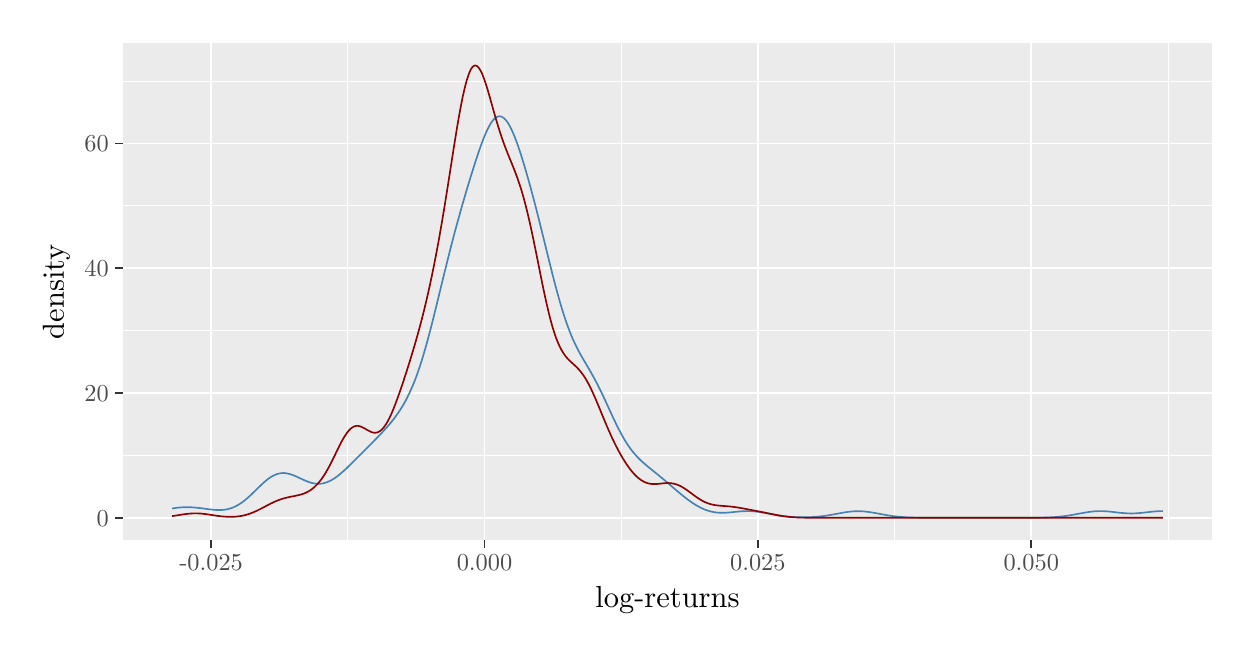
\begin{tikzpicture}[x=1pt,y=1pt]
\definecolor{fillColor}{RGB}{255,255,255}
\path[use as bounding box,fill=fillColor,fill opacity=0.00] (0,0) rectangle (433.62,216.81);
\begin{scope}
\path[clip] (  0.00,  0.00) rectangle (433.62,216.81);
\definecolor{drawColor}{RGB}{255,255,255}
\definecolor{fillColor}{RGB}{255,255,255}

\path[draw=drawColor,line width= 0.6pt,line join=round,line cap=round,fill=fillColor] (  0.00,  0.00) rectangle (433.62,216.81);
\end{scope}
\begin{scope}
\path[clip] ( 34.27, 31.53) rectangle (428.12,211.31);
\definecolor{fillColor}{gray}{0.92}

\path[fill=fillColor] ( 34.27, 31.53) rectangle (428.12,211.31);
\definecolor{drawColor}{RGB}{255,255,255}

\path[draw=drawColor,line width= 0.3pt,line join=round] ( 34.27, 62.24) --
	(428.12, 62.24);

\path[draw=drawColor,line width= 0.3pt,line join=round] ( 34.27,107.32) --
	(428.12,107.32);

\path[draw=drawColor,line width= 0.3pt,line join=round] ( 34.27,152.40) --
	(428.12,152.40);

\path[draw=drawColor,line width= 0.3pt,line join=round] ( 34.27,197.48) --
	(428.12,197.48);

\path[draw=drawColor,line width= 0.3pt,line join=round] (115.67, 31.53) --
	(115.67,211.31);

\path[draw=drawColor,line width= 0.3pt,line join=round] (214.46, 31.53) --
	(214.46,211.31);

\path[draw=drawColor,line width= 0.3pt,line join=round] (313.25, 31.53) --
	(313.25,211.31);

\path[draw=drawColor,line width= 0.3pt,line join=round] (412.03, 31.53) --
	(412.03,211.31);

\path[draw=drawColor,line width= 0.6pt,line join=round] ( 34.27, 39.70) --
	(428.12, 39.70);

\path[draw=drawColor,line width= 0.6pt,line join=round] ( 34.27, 84.78) --
	(428.12, 84.78);

\path[draw=drawColor,line width= 0.6pt,line join=round] ( 34.27,129.86) --
	(428.12,129.86);

\path[draw=drawColor,line width= 0.6pt,line join=round] ( 34.27,174.94) --
	(428.12,174.94);

\path[draw=drawColor,line width= 0.6pt,line join=round] ( 66.28, 31.53) --
	( 66.28,211.31);

\path[draw=drawColor,line width= 0.6pt,line join=round] (165.07, 31.53) --
	(165.07,211.31);

\path[draw=drawColor,line width= 0.6pt,line join=round] (263.85, 31.53) --
	(263.85,211.31);

\path[draw=drawColor,line width= 0.6pt,line join=round] (362.64, 31.53) --
	(362.64,211.31);
\definecolor{drawColor}{RGB}{70,130,180}

\path[draw=drawColor,line width= 0.6pt,line join=round] ( 52.17, 43.06) --
	( 52.87, 43.17) --
	( 53.57, 43.27) --
	( 54.27, 43.36) --
	( 54.97, 43.42) --
	( 55.67, 43.47) --
	( 56.37, 43.51) --
	( 57.07, 43.53) --
	( 57.78, 43.53) --
	( 58.48, 43.52) --
	( 59.18, 43.49) --
	( 59.88, 43.45) --
	( 60.58, 43.39) --
	( 61.28, 43.33) --
	( 61.98, 43.25) --
	( 62.68, 43.17) --
	( 63.38, 43.07) --
	( 64.08, 42.98) --
	( 64.78, 42.88) --
	( 65.48, 42.79) --
	( 66.18, 42.71) --
	( 66.88, 42.63) --
	( 67.59, 42.57) --
	( 68.29, 42.52) --
	( 68.99, 42.50) --
	( 69.69, 42.51) --
	( 70.39, 42.55) --
	( 71.09, 42.62) --
	( 71.79, 42.73) --
	( 72.49, 42.88) --
	( 73.19, 43.07) --
	( 73.89, 43.31) --
	( 74.59, 43.60) --
	( 75.29, 43.94) --
	( 75.99, 44.32) --
	( 76.69, 44.75) --
	( 77.39, 45.22) --
	( 78.10, 45.74) --
	( 78.80, 46.31) --
	( 79.50, 46.91) --
	( 80.20, 47.54) --
	( 80.90, 48.19) --
	( 81.60, 48.87) --
	( 82.30, 49.55) --
	( 83.00, 50.24) --
	( 83.70, 50.92) --
	( 84.40, 51.59) --
	( 85.10, 52.24) --
	( 85.80, 52.86) --
	( 86.50, 53.44) --
	( 87.20, 53.97) --
	( 87.90, 54.44) --
	( 88.61, 54.85) --
	( 89.31, 55.19) --
	( 90.01, 55.47) --
	( 90.71, 55.67) --
	( 91.41, 55.81) --
	( 92.11, 55.87) --
	( 92.81, 55.86) --
	( 93.51, 55.78) --
	( 94.21, 55.64) --
	( 94.91, 55.45) --
	( 95.61, 55.22) --
	( 96.31, 54.95) --
	( 97.01, 54.65) --
	( 97.71, 54.33) --
	( 98.42, 54.00) --
	( 99.12, 53.67) --
	( 99.82, 53.35) --
	(100.52, 53.05) --
	(101.22, 52.77) --
	(101.92, 52.52) --
	(102.62, 52.32) --
	(103.32, 52.16) --
	(104.02, 52.05) --
	(104.72, 51.99) --
	(105.42, 51.99) --
	(106.12, 52.05) --
	(106.82, 52.16) --
	(107.52, 52.35) --
	(108.22, 52.59) --
	(108.93, 52.89) --
	(109.63, 53.24) --
	(110.33, 53.64) --
	(111.03, 54.09) --
	(111.73, 54.59) --
	(112.43, 55.14) --
	(113.13, 55.71) --
	(113.83, 56.32) --
	(114.53, 56.95) --
	(115.23, 57.60) --
	(115.93, 58.27) --
	(116.63, 58.96) --
	(117.33, 59.65) --
	(118.03, 60.35) --
	(118.73, 61.05) --
	(119.44, 61.75) --
	(120.14, 62.46) --
	(120.84, 63.16) --
	(121.54, 63.86) --
	(122.24, 64.56) --
	(122.94, 65.26) --
	(123.64, 65.96) --
	(124.34, 66.67) --
	(125.04, 67.37) --
	(125.74, 68.09) --
	(126.44, 68.81) --
	(127.14, 69.53) --
	(127.84, 70.27) --
	(128.54, 71.03) --
	(129.24, 71.80) --
	(129.95, 72.59) --
	(130.65, 73.40) --
	(131.35, 74.24) --
	(132.05, 75.12) --
	(132.75, 76.04) --
	(133.45, 77.00) --
	(134.15, 78.01) --
	(134.85, 79.08) --
	(135.55, 80.22) --
	(136.25, 81.44) --
	(136.95, 82.75) --
	(137.65, 84.15) --
	(138.35, 85.65) --
	(139.05, 87.26) --
	(139.76, 88.97) --
	(140.46, 90.81) --
	(141.16, 92.79) --
	(141.86, 94.88) --
	(142.56, 97.09) --
	(143.26, 99.42) --
	(143.96,101.85) --
	(144.66,104.39) --
	(145.36,107.03) --
	(146.06,109.75) --
	(146.76,112.53) --
	(147.46,115.36) --
	(148.16,118.23) --
	(148.86,121.12) --
	(149.56,124.01) --
	(150.27,126.90) --
	(150.97,129.75) --
	(151.67,132.58) --
	(152.37,135.37) --
	(153.07,138.11) --
	(153.77,140.80) --
	(154.47,143.44) --
	(155.17,146.02) --
	(155.87,148.55) --
	(156.57,151.04) --
	(157.27,153.49) --
	(157.97,155.89) --
	(158.67,158.27) --
	(159.37,160.60) --
	(160.07,162.90) --
	(160.78,165.16) --
	(161.48,167.38) --
	(162.18,169.55) --
	(162.88,171.65) --
	(163.58,173.67) --
	(164.28,175.59) --
	(164.98,177.37) --
	(165.68,179.02) --
	(166.38,180.49) --
	(167.08,181.79) --
	(167.78,182.88) --
	(168.48,183.75) --
	(169.18,184.37) --
	(169.88,184.71) --
	(170.59,184.79) --
	(171.29,184.62) --
	(171.99,184.20) --
	(172.69,183.53) --
	(173.39,182.63) --
	(174.09,181.47) --
	(174.79,180.10) --
	(175.49,178.53) --
	(176.19,176.81) --
	(176.89,174.93) --
	(177.59,172.91) --
	(178.29,170.78) --
	(178.99,168.54) --
	(179.69,166.20) --
	(180.39,163.78) --
	(181.10,161.30) --
	(181.80,158.75) --
	(182.50,156.14) --
	(183.20,153.48) --
	(183.90,150.77) --
	(184.60,148.01) --
	(185.30,145.21) --
	(186.00,142.39) --
	(186.70,139.55) --
	(187.40,136.70) --
	(188.10,133.85) --
	(188.80,131.02) --
	(189.50,128.23) --
	(190.20,125.49) --
	(190.90,122.83) --
	(191.61,120.24) --
	(192.31,117.75) --
	(193.01,115.37) --
	(193.71,113.13) --
	(194.41,111.01) --
	(195.11,109.02) --
	(195.81,107.16) --
	(196.51,105.42) --
	(197.21,103.80) --
	(197.91,102.30) --
	(198.61,100.90) --
	(199.31, 99.57) --
	(200.01, 98.30) --
	(200.71, 97.07) --
	(201.42, 95.88) --
	(202.12, 94.69) --
	(202.82, 93.49) --
	(203.52, 92.28) --
	(204.22, 91.03) --
	(204.92, 89.74) --
	(205.62, 88.42) --
	(206.32, 87.04) --
	(207.02, 85.63) --
	(207.72, 84.17) --
	(208.42, 82.68) --
	(209.12, 81.16) --
	(209.82, 79.64) --
	(210.52, 78.11) --
	(211.22, 76.59) --
	(211.93, 75.09) --
	(212.63, 73.63) --
	(213.33, 72.22) --
	(214.03, 70.87) --
	(214.73, 69.57) --
	(215.43, 68.33) --
	(216.13, 67.17) --
	(216.83, 66.08) --
	(217.53, 65.07) --
	(218.23, 64.12) --
	(218.93, 63.25) --
	(219.63, 62.43) --
	(220.33, 61.66) --
	(221.03, 60.94) --
	(221.73, 60.27) --
	(222.44, 59.63) --
	(223.14, 59.02) --
	(223.84, 58.43) --
	(224.54, 57.85) --
	(225.24, 57.28) --
	(225.94, 56.71) --
	(226.64, 56.15) --
	(227.34, 55.59) --
	(228.04, 55.01) --
	(228.74, 54.44) --
	(229.44, 53.86) --
	(230.14, 53.27) --
	(230.84, 52.67) --
	(231.54, 52.08) --
	(232.24, 51.48) --
	(232.95, 50.87) --
	(233.65, 50.27) --
	(234.35, 49.67) --
	(235.05, 49.08) --
	(235.75, 48.50) --
	(236.45, 47.92) --
	(237.15, 47.36) --
	(237.85, 46.81) --
	(238.55, 46.28) --
	(239.25, 45.77) --
	(239.95, 45.28) --
	(240.65, 44.81) --
	(241.35, 44.37) --
	(242.05, 43.96) --
	(242.76, 43.58) --
	(243.46, 43.22) --
	(244.16, 42.90) --
	(244.86, 42.61) --
	(245.56, 42.36) --
	(246.26, 42.14) --
	(246.96, 41.96) --
	(247.66, 41.81) --
	(248.36, 41.69) --
	(249.06, 41.60) --
	(249.76, 41.54) --
	(250.46, 41.51) --
	(251.16, 41.50) --
	(251.86, 41.52) --
	(252.56, 41.56) --
	(253.27, 41.61) --
	(253.97, 41.67) --
	(254.67, 41.73) --
	(255.37, 41.81) --
	(256.07, 41.88) --
	(256.77, 41.95) --
	(257.47, 42.01) --
	(258.17, 42.05) --
	(258.87, 42.09) --
	(259.57, 42.12) --
	(260.27, 42.12) --
	(260.97, 42.11) --
	(261.67, 42.08) --
	(262.37, 42.03) --
	(263.07, 41.97) --
	(263.78, 41.89) --
	(264.48, 41.79) --
	(265.18, 41.69) --
	(265.88, 41.57) --
	(266.58, 41.45) --
	(267.28, 41.32) --
	(267.98, 41.19) --
	(268.68, 41.06) --
	(269.38, 40.93) --
	(270.08, 40.80) --
	(270.78, 40.68) --
	(271.48, 40.56) --
	(272.18, 40.46) --
	(272.88, 40.36) --
	(273.59, 40.27) --
	(274.29, 40.19) --
	(274.99, 40.12) --
	(275.69, 40.06) --
	(276.39, 40.01) --
	(277.09, 39.96) --
	(277.79, 39.93) --
	(278.49, 39.90) --
	(279.19, 39.89) --
	(279.89, 39.88) --
	(280.59, 39.88) --
	(281.29, 39.89) --
	(281.99, 39.90) --
	(282.69, 39.93) --
	(283.39, 39.96) --
	(284.10, 40.00) --
	(284.80, 40.05) --
	(285.50, 40.11) --
	(286.20, 40.18) --
	(286.90, 40.26) --
	(287.60, 40.35) --
	(288.30, 40.45) --
	(289.00, 40.55) --
	(289.70, 40.67) --
	(290.40, 40.79) --
	(291.10, 40.91) --
	(291.80, 41.04) --
	(292.50, 41.17) --
	(293.20, 41.30) --
	(293.90, 41.43) --
	(294.61, 41.56) --
	(295.31, 41.67) --
	(296.01, 41.78) --
	(296.71, 41.87) --
	(297.41, 41.95) --
	(298.11, 42.01) --
	(298.81, 42.06) --
	(299.51, 42.08) --
	(300.21, 42.09) --
	(300.91, 42.07) --
	(301.61, 42.04) --
	(302.31, 41.99) --
	(303.01, 41.92) --
	(303.71, 41.83) --
	(304.41, 41.73) --
	(305.12, 41.62) --
	(305.82, 41.50) --
	(306.52, 41.38) --
	(307.22, 41.25) --
	(307.92, 41.12) --
	(308.62, 40.99) --
	(309.32, 40.86) --
	(310.02, 40.73) --
	(310.72, 40.61) --
	(311.42, 40.50) --
	(312.12, 40.40) --
	(312.82, 40.30) --
	(313.52, 40.22) --
	(314.22, 40.14) --
	(314.93, 40.07) --
	(315.63, 40.01) --
	(316.33, 39.96) --
	(317.03, 39.91) --
	(317.73, 39.87) --
	(318.43, 39.84) --
	(319.13, 39.81) --
	(319.83, 39.79) --
	(320.53, 39.77) --
	(321.23, 39.76) --
	(321.93, 39.74) --
	(322.63, 39.73) --
	(323.33, 39.73) --
	(324.03, 39.72) --
	(324.73, 39.72) --
	(325.44, 39.71) --
	(326.14, 39.71) --
	(326.84, 39.71) --
	(327.54, 39.71) --
	(328.24, 39.71) --
	(328.94, 39.70) --
	(329.64, 39.70) --
	(330.34, 39.70) --
	(331.04, 39.70) --
	(331.74, 39.70) --
	(332.44, 39.70) --
	(333.14, 39.70) --
	(333.84, 39.70) --
	(334.54, 39.70) --
	(335.24, 39.70) --
	(335.95, 39.70) --
	(336.65, 39.70) --
	(337.35, 39.70) --
	(338.05, 39.70) --
	(338.75, 39.70) --
	(339.45, 39.70) --
	(340.15, 39.70) --
	(340.85, 39.70) --
	(341.55, 39.70) --
	(342.25, 39.70) --
	(342.95, 39.70) --
	(343.65, 39.70) --
	(344.35, 39.70) --
	(345.05, 39.70) --
	(345.76, 39.70) --
	(346.46, 39.70) --
	(347.16, 39.70) --
	(347.86, 39.70) --
	(348.56, 39.70) --
	(349.26, 39.70) --
	(349.96, 39.70) --
	(350.66, 39.70) --
	(351.36, 39.70) --
	(352.06, 39.70) --
	(352.76, 39.70) --
	(353.46, 39.70) --
	(354.16, 39.70) --
	(354.86, 39.70) --
	(355.56, 39.70) --
	(356.27, 39.70) --
	(356.97, 39.70) --
	(357.67, 39.70) --
	(358.37, 39.70) --
	(359.07, 39.71) --
	(359.77, 39.71) --
	(360.47, 39.71) --
	(361.17, 39.71) --
	(361.87, 39.71) --
	(362.57, 39.72) --
	(363.27, 39.72) --
	(363.97, 39.73) --
	(364.67, 39.73) --
	(365.37, 39.74) --
	(366.07, 39.75) --
	(366.78, 39.77) --
	(367.48, 39.79) --
	(368.18, 39.81) --
	(368.88, 39.84) --
	(369.58, 39.87) --
	(370.28, 39.90) --
	(370.98, 39.95) --
	(371.68, 40.00) --
	(372.38, 40.06) --
	(373.08, 40.13) --
	(373.78, 40.21) --
	(374.48, 40.29) --
	(375.18, 40.38) --
	(375.88, 40.49) --
	(376.58, 40.60) --
	(377.29, 40.72) --
	(377.99, 40.84) --
	(378.69, 40.97) --
	(379.39, 41.10) --
	(380.09, 41.23) --
	(380.79, 41.36) --
	(381.49, 41.49) --
	(382.19, 41.61) --
	(382.89, 41.72) --
	(383.59, 41.83) --
	(384.29, 41.92) --
	(384.99, 41.99) --
	(385.69, 42.05) --
	(386.39, 42.09) --
	(387.10, 42.11) --
	(387.80, 42.12) --
	(388.50, 42.11) --
	(389.20, 42.08) --
	(389.90, 42.03) --
	(390.60, 41.97) --
	(391.30, 41.91) --
	(392.00, 41.83) --
	(392.70, 41.75) --
	(393.40, 41.67) --
	(394.10, 41.59) --
	(394.80, 41.51) --
	(395.50, 41.44) --
	(396.20, 41.38) --
	(396.90, 41.34) --
	(397.61, 41.30) --
	(398.31, 41.28) --
	(399.01, 41.28) --
	(399.71, 41.29) --
	(400.41, 41.32) --
	(401.11, 41.37) --
	(401.81, 41.42) --
	(402.51, 41.49) --
	(403.21, 41.56) --
	(403.91, 41.64) --
	(404.61, 41.72) --
	(405.31, 41.80) --
	(406.01, 41.88) --
	(406.71, 41.95) --
	(407.41, 42.01) --
	(408.12, 42.06) --
	(408.82, 42.10) --
	(409.52, 42.11) --
	(410.22, 42.11);
\definecolor{drawColor}{RGB}{139,0,0}

\path[draw=drawColor,line width= 0.6pt,line join=round] ( 52.17, 40.31) --
	( 52.87, 40.41) --
	( 53.57, 40.51) --
	( 54.27, 40.63) --
	( 54.97, 40.74) --
	( 55.67, 40.85) --
	( 56.37, 40.95) --
	( 57.07, 41.05) --
	( 57.78, 41.14) --
	( 58.48, 41.21) --
	( 59.18, 41.26) --
	( 59.88, 41.30) --
	( 60.58, 41.31) --
	( 61.28, 41.30) --
	( 61.98, 41.27) --
	( 62.68, 41.22) --
	( 63.38, 41.15) --
	( 64.08, 41.07) --
	( 64.78, 40.98) --
	( 65.48, 40.88) --
	( 66.18, 40.77) --
	( 66.88, 40.66) --
	( 67.59, 40.55) --
	( 68.29, 40.45) --
	( 68.99, 40.35) --
	( 69.69, 40.27) --
	( 70.39, 40.19) --
	( 71.09, 40.13) --
	( 71.79, 40.09) --
	( 72.49, 40.06) --
	( 73.19, 40.05) --
	( 73.89, 40.06) --
	( 74.59, 40.09) --
	( 75.29, 40.13) --
	( 75.99, 40.21) --
	( 76.69, 40.30) --
	( 77.39, 40.42) --
	( 78.10, 40.57) --
	( 78.80, 40.74) --
	( 79.50, 40.94) --
	( 80.20, 41.17) --
	( 80.90, 41.43) --
	( 81.60, 41.71) --
	( 82.30, 42.02) --
	( 83.00, 42.34) --
	( 83.70, 42.69) --
	( 84.40, 43.04) --
	( 85.10, 43.41) --
	( 85.80, 43.78) --
	( 86.50, 44.16) --
	( 87.20, 44.52) --
	( 87.90, 44.88) --
	( 88.61, 45.22) --
	( 89.31, 45.54) --
	( 90.01, 45.84) --
	( 90.71, 46.12) --
	( 91.41, 46.37) --
	( 92.11, 46.59) --
	( 92.81, 46.79) --
	( 93.51, 46.97) --
	( 94.21, 47.13) --
	( 94.91, 47.28) --
	( 95.61, 47.42) --
	( 96.31, 47.55) --
	( 97.01, 47.70) --
	( 97.71, 47.85) --
	( 98.42, 48.03) --
	( 99.12, 48.24) --
	( 99.82, 48.48) --
	(100.52, 48.77) --
	(101.22, 49.11) --
	(101.92, 49.51) --
	(102.62, 49.99) --
	(103.32, 50.55) --
	(104.02, 51.18) --
	(104.72, 51.91) --
	(105.42, 52.72) --
	(106.12, 53.63) --
	(106.82, 54.63) --
	(107.52, 55.72) --
	(108.22, 56.92) --
	(108.93, 58.20) --
	(109.63, 59.55) --
	(110.33, 60.95) --
	(111.03, 62.38) --
	(111.73, 63.83) --
	(112.43, 65.26) --
	(113.13, 66.64) --
	(113.83, 67.95) --
	(114.53, 69.14) --
	(115.23, 70.20) --
	(115.93, 71.10) --
	(116.63, 71.83) --
	(117.33, 72.37) --
	(118.03, 72.73) --
	(118.73, 72.91) --
	(119.44, 72.91) --
	(120.14, 72.74) --
	(120.84, 72.47) --
	(121.54, 72.11) --
	(122.24, 71.71) --
	(122.94, 71.30) --
	(123.64, 70.94) --
	(124.34, 70.64) --
	(125.04, 70.45) --
	(125.74, 70.43) --
	(126.44, 70.58) --
	(127.14, 70.92) --
	(127.84, 71.46) --
	(128.54, 72.21) --
	(129.24, 73.15) --
	(129.95, 74.29) --
	(130.65, 75.61) --
	(131.35, 77.10) --
	(132.05, 78.74) --
	(132.75, 80.51) --
	(133.45, 82.37) --
	(134.15, 84.32) --
	(134.85, 86.33) --
	(135.55, 88.41) --
	(136.25, 90.53) --
	(136.95, 92.69) --
	(137.65, 94.90) --
	(138.35, 97.16) --
	(139.05, 99.47) --
	(139.76,101.83) --
	(140.46,104.26) --
	(141.16,106.77) --
	(141.86,109.35) --
	(142.56,112.03) --
	(143.26,114.81) --
	(143.96,117.72) --
	(144.66,120.75) --
	(145.36,123.90) --
	(146.06,127.19) --
	(146.76,130.62) --
	(147.46,134.19) --
	(148.16,137.92) --
	(148.86,141.79) --
	(149.56,145.83) --
	(150.27,150.01) --
	(150.97,154.30) --
	(151.67,158.70) --
	(152.37,163.16) --
	(153.07,167.65) --
	(153.77,172.13) --
	(154.47,176.54) --
	(155.17,180.82) --
	(155.87,184.88) --
	(156.57,188.67) --
	(157.27,192.14) --
	(157.97,195.21) --
	(158.67,197.85) --
	(159.37,199.99) --
	(160.07,201.62) --
	(160.78,202.68) --
	(161.48,203.14) --
	(162.18,203.06) --
	(162.88,202.48) --
	(163.58,201.44) --
	(164.28,199.99) --
	(164.98,198.18) --
	(165.68,196.10) --
	(166.38,193.80) --
	(167.08,191.36) --
	(167.78,188.85) --
	(168.48,186.35) --
	(169.18,183.90) --
	(169.88,181.54) --
	(170.59,179.29) --
	(171.29,177.16) --
	(171.99,175.16) --
	(172.69,173.29) --
	(173.39,171.50) --
	(174.09,169.78) --
	(174.79,168.07) --
	(175.49,166.34) --
	(176.19,164.55) --
	(176.89,162.67) --
	(177.59,160.66) --
	(178.29,158.49) --
	(178.99,156.12) --
	(179.69,153.55) --
	(180.39,150.78) --
	(181.10,147.83) --
	(181.80,144.71) --
	(182.50,141.44) --
	(183.20,138.05) --
	(183.90,134.58) --
	(184.60,131.07) --
	(185.30,127.57) --
	(186.00,124.13) --
	(186.70,120.79) --
	(187.40,117.59) --
	(188.10,114.57) --
	(188.80,111.75) --
	(189.50,109.17) --
	(190.20,106.84) --
	(190.90,104.80) --
	(191.61,103.01) --
	(192.31,101.45) --
	(193.01,100.13) --
	(193.71, 99.00) --
	(194.41, 98.04) --
	(195.11, 97.22) --
	(195.81, 96.50) --
	(196.51, 95.85) --
	(197.21, 95.22) --
	(197.91, 94.57) --
	(198.61, 93.88) --
	(199.31, 93.13) --
	(200.01, 92.28) --
	(200.71, 91.33) --
	(201.42, 90.27) --
	(202.12, 89.09) --
	(202.82, 87.79) --
	(203.52, 86.38) --
	(204.22, 84.88) --
	(204.92, 83.31) --
	(205.62, 81.68) --
	(206.32, 80.01) --
	(207.02, 78.31) --
	(207.72, 76.60) --
	(208.42, 74.91) --
	(209.12, 73.24) --
	(209.82, 71.61) --
	(210.52, 70.03) --
	(211.22, 68.49) --
	(211.93, 67.02) --
	(212.63, 65.60) --
	(213.33, 64.24) --
	(214.03, 62.95) --
	(214.73, 61.73) --
	(215.43, 60.57) --
	(216.13, 59.48) --
	(216.83, 58.45) --
	(217.53, 57.49) --
	(218.23, 56.59) --
	(218.93, 55.77) --
	(219.63, 55.03) --
	(220.33, 54.37) --
	(221.03, 53.79) --
	(221.73, 53.29) --
	(222.44, 52.87) --
	(223.14, 52.53) --
	(223.84, 52.27) --
	(224.54, 52.08) --
	(225.24, 51.96) --
	(225.94, 51.90) --
	(226.64, 51.90) --
	(227.34, 51.93) --
	(228.04, 51.99) --
	(228.74, 52.06) --
	(229.44, 52.14) --
	(230.14, 52.20) --
	(230.84, 52.25) --
	(231.54, 52.26) --
	(232.24, 52.22) --
	(232.95, 52.13) --
	(233.65, 51.99) --
	(234.35, 51.79) --
	(235.05, 51.54) --
	(235.75, 51.22) --
	(236.45, 50.85) --
	(237.15, 50.43) --
	(237.85, 49.97) --
	(238.55, 49.47) --
	(239.25, 48.96) --
	(239.95, 48.44) --
	(240.65, 47.92) --
	(241.35, 47.41) --
	(242.05, 46.92) --
	(242.76, 46.46) --
	(243.46, 46.03) --
	(244.16, 45.66) --
	(244.86, 45.32) --
	(245.56, 45.03) --
	(246.26, 44.79) --
	(246.96, 44.59) --
	(247.66, 44.42) --
	(248.36, 44.29) --
	(249.06, 44.19) --
	(249.76, 44.12) --
	(250.46, 44.06) --
	(251.16, 44.00) --
	(251.86, 43.95) --
	(252.56, 43.90) --
	(253.27, 43.84) --
	(253.97, 43.77) --
	(254.67, 43.69) --
	(255.37, 43.60) --
	(256.07, 43.50) --
	(256.77, 43.39) --
	(257.47, 43.27) --
	(258.17, 43.15) --
	(258.87, 43.02) --
	(259.57, 42.89) --
	(260.27, 42.75) --
	(260.97, 42.62) --
	(261.67, 42.49) --
	(262.37, 42.35) --
	(263.07, 42.22) --
	(263.78, 42.08) --
	(264.48, 41.95) --
	(265.18, 41.81) --
	(265.88, 41.67) --
	(266.58, 41.52) --
	(267.28, 41.37) --
	(267.98, 41.23) --
	(268.68, 41.08) --
	(269.38, 40.94) --
	(270.08, 40.80) --
	(270.78, 40.66) --
	(271.48, 40.53) --
	(272.18, 40.42) --
	(272.88, 40.31) --
	(273.59, 40.21) --
	(274.29, 40.12) --
	(274.99, 40.05) --
	(275.69, 39.98) --
	(276.39, 39.92) --
	(277.09, 39.88) --
	(277.79, 39.84) --
	(278.49, 39.80) --
	(279.19, 39.78) --
	(279.89, 39.76) --
	(280.59, 39.75) --
	(281.29, 39.73) --
	(281.99, 39.72) --
	(282.69, 39.72) --
	(283.39, 39.71) --
	(284.10, 39.71) --
	(284.80, 39.71) --
	(285.50, 39.71) --
	(286.20, 39.70) --
	(286.90, 39.70) --
	(287.60, 39.70) --
	(288.30, 39.70) --
	(289.00, 39.70) --
	(289.70, 39.70) --
	(290.40, 39.70) --
	(291.10, 39.70) --
	(291.80, 39.70) --
	(292.50, 39.70) --
	(293.20, 39.70) --
	(293.90, 39.70) --
	(294.61, 39.70) --
	(295.31, 39.70) --
	(296.01, 39.70) --
	(296.71, 39.70) --
	(297.41, 39.70) --
	(298.11, 39.70) --
	(298.81, 39.70) --
	(299.51, 39.70) --
	(300.21, 39.70) --
	(300.91, 39.70) --
	(301.61, 39.70) --
	(302.31, 39.70) --
	(303.01, 39.70) --
	(303.71, 39.70) --
	(304.41, 39.70) --
	(305.12, 39.70) --
	(305.82, 39.70) --
	(306.52, 39.70) --
	(307.22, 39.70) --
	(307.92, 39.70) --
	(308.62, 39.70) --
	(309.32, 39.70) --
	(310.02, 39.70) --
	(310.72, 39.70) --
	(311.42, 39.70) --
	(312.12, 39.70) --
	(312.82, 39.70) --
	(313.52, 39.70) --
	(314.22, 39.70) --
	(314.93, 39.70) --
	(315.63, 39.70) --
	(316.33, 39.70) --
	(317.03, 39.70) --
	(317.73, 39.70) --
	(318.43, 39.70) --
	(319.13, 39.70) --
	(319.83, 39.70) --
	(320.53, 39.70) --
	(321.23, 39.70) --
	(321.93, 39.70) --
	(322.63, 39.70) --
	(323.33, 39.70) --
	(324.03, 39.70) --
	(324.73, 39.70) --
	(325.44, 39.70) --
	(326.14, 39.70) --
	(326.84, 39.70) --
	(327.54, 39.70) --
	(328.24, 39.70) --
	(328.94, 39.70) --
	(329.64, 39.70) --
	(330.34, 39.70) --
	(331.04, 39.70) --
	(331.74, 39.70) --
	(332.44, 39.70) --
	(333.14, 39.70) --
	(333.84, 39.70) --
	(334.54, 39.70) --
	(335.24, 39.70) --
	(335.95, 39.70) --
	(336.65, 39.70) --
	(337.35, 39.70) --
	(338.05, 39.70) --
	(338.75, 39.70) --
	(339.45, 39.70) --
	(340.15, 39.70) --
	(340.85, 39.70) --
	(341.55, 39.70) --
	(342.25, 39.70) --
	(342.95, 39.70) --
	(343.65, 39.70) --
	(344.35, 39.70) --
	(345.05, 39.70) --
	(345.76, 39.70) --
	(346.46, 39.70) --
	(347.16, 39.70) --
	(347.86, 39.70) --
	(348.56, 39.70) --
	(349.26, 39.70) --
	(349.96, 39.70) --
	(350.66, 39.70) --
	(351.36, 39.70) --
	(352.06, 39.70) --
	(352.76, 39.70) --
	(353.46, 39.70) --
	(354.16, 39.70) --
	(354.86, 39.70) --
	(355.56, 39.70) --
	(356.27, 39.70) --
	(356.97, 39.70) --
	(357.67, 39.70) --
	(358.37, 39.70) --
	(359.07, 39.70) --
	(359.77, 39.70) --
	(360.47, 39.70) --
	(361.17, 39.70) --
	(361.87, 39.70) --
	(362.57, 39.70) --
	(363.27, 39.70) --
	(363.97, 39.70) --
	(364.67, 39.70) --
	(365.37, 39.70) --
	(366.07, 39.70) --
	(366.78, 39.70) --
	(367.48, 39.70) --
	(368.18, 39.70) --
	(368.88, 39.70) --
	(369.58, 39.70) --
	(370.28, 39.70) --
	(370.98, 39.70) --
	(371.68, 39.70) --
	(372.38, 39.70) --
	(373.08, 39.70) --
	(373.78, 39.70) --
	(374.48, 39.70) --
	(375.18, 39.70) --
	(375.88, 39.70) --
	(376.58, 39.70) --
	(377.29, 39.70) --
	(377.99, 39.70) --
	(378.69, 39.70) --
	(379.39, 39.70) --
	(380.09, 39.70) --
	(380.79, 39.70) --
	(381.49, 39.70) --
	(382.19, 39.70) --
	(382.89, 39.70) --
	(383.59, 39.70) --
	(384.29, 39.70) --
	(384.99, 39.70) --
	(385.69, 39.70) --
	(386.39, 39.70) --
	(387.10, 39.70) --
	(387.80, 39.70) --
	(388.50, 39.70) --
	(389.20, 39.70) --
	(389.90, 39.70) --
	(390.60, 39.70) --
	(391.30, 39.70) --
	(392.00, 39.70) --
	(392.70, 39.70) --
	(393.40, 39.70) --
	(394.10, 39.70) --
	(394.80, 39.70) --
	(395.50, 39.70) --
	(396.20, 39.70) --
	(396.90, 39.70) --
	(397.61, 39.70) --
	(398.31, 39.70) --
	(399.01, 39.70) --
	(399.71, 39.70) --
	(400.41, 39.70) --
	(401.11, 39.70) --
	(401.81, 39.70) --
	(402.51, 39.70) --
	(403.21, 39.70) --
	(403.91, 39.70) --
	(404.61, 39.70) --
	(405.31, 39.70) --
	(406.01, 39.70) --
	(406.71, 39.70) --
	(407.41, 39.70) --
	(408.12, 39.70) --
	(408.82, 39.70) --
	(409.52, 39.70) --
	(410.22, 39.70);
\end{scope}
\begin{scope}
\path[clip] (  0.00,  0.00) rectangle (433.62,216.81);
\definecolor{drawColor}{gray}{0.30}

\node[text=drawColor,anchor=base east,inner sep=0pt, outer sep=0pt, scale=  0.88] at ( 29.32, 36.67) {0};

\node[text=drawColor,anchor=base east,inner sep=0pt, outer sep=0pt, scale=  0.88] at ( 29.32, 81.75) {20};

\node[text=drawColor,anchor=base east,inner sep=0pt, outer sep=0pt, scale=  0.88] at ( 29.32,126.83) {40};

\node[text=drawColor,anchor=base east,inner sep=0pt, outer sep=0pt, scale=  0.88] at ( 29.32,171.91) {60};
\end{scope}
\begin{scope}
\path[clip] (  0.00,  0.00) rectangle (433.62,216.81);
\definecolor{drawColor}{gray}{0.20}

\path[draw=drawColor,line width= 0.6pt,line join=round] ( 31.52, 39.70) --
	( 34.27, 39.70);

\path[draw=drawColor,line width= 0.6pt,line join=round] ( 31.52, 84.78) --
	( 34.27, 84.78);

\path[draw=drawColor,line width= 0.6pt,line join=round] ( 31.52,129.86) --
	( 34.27,129.86);

\path[draw=drawColor,line width= 0.6pt,line join=round] ( 31.52,174.94) --
	( 34.27,174.94);
\end{scope}
\begin{scope}
\path[clip] (  0.00,  0.00) rectangle (433.62,216.81);
\definecolor{drawColor}{gray}{0.20}

\path[draw=drawColor,line width= 0.6pt,line join=round] ( 66.28, 28.78) --
	( 66.28, 31.53);

\path[draw=drawColor,line width= 0.6pt,line join=round] (165.07, 28.78) --
	(165.07, 31.53);

\path[draw=drawColor,line width= 0.6pt,line join=round] (263.85, 28.78) --
	(263.85, 31.53);

\path[draw=drawColor,line width= 0.6pt,line join=round] (362.64, 28.78) --
	(362.64, 31.53);
\end{scope}
\begin{scope}
\path[clip] (  0.00,  0.00) rectangle (433.62,216.81);
\definecolor{drawColor}{gray}{0.30}

\node[text=drawColor,anchor=base,inner sep=0pt, outer sep=0pt, scale=  0.88] at ( 66.28, 20.52) {-0.025};

\node[text=drawColor,anchor=base,inner sep=0pt, outer sep=0pt, scale=  0.88] at (165.07, 20.52) {0.000};

\node[text=drawColor,anchor=base,inner sep=0pt, outer sep=0pt, scale=  0.88] at (263.85, 20.52) {0.025};

\node[text=drawColor,anchor=base,inner sep=0pt, outer sep=0pt, scale=  0.88] at (362.64, 20.52) {0.050};
\end{scope}
\begin{scope}
\path[clip] (  0.00,  0.00) rectangle (433.62,216.81);
\definecolor{drawColor}{RGB}{0,0,0}

\node[text=drawColor,anchor=base,inner sep=0pt, outer sep=0pt, scale=  1.10] at (231.19,  7.44) {log-returns};
\end{scope}
\begin{scope}
\path[clip] (  0.00,  0.00) rectangle (433.62,216.81);
\definecolor{drawColor}{RGB}{0,0,0}

\node[text=drawColor,rotate= 90.00,anchor=base,inner sep=0pt, outer sep=0pt, scale=  1.10] at ( 13.08,121.42) {density};
\end{scope}
\end{tikzpicture}

  \caption{Historical and HSV related Apple stock Log-returns distribution}
  \floatfoot{The above blue density curve is constructed over the historical data of the Apple share of stock price evolution from 18th May 2017 to 18th May 2018. while the red curve is constructed from time-series genereated by the function \textit{hsv\_ts} taking the risk-neutral parameters \ref{eq:methodology:arg:heston:riskneutral} as arguments.
  }
  \label{p:methodology:density:aapl:heston:riskneutral}
\end{figure}


The goal of that section is to find the risk-averse parameters that make both the distributions of the log-returns generated from market data or from \textit{hsv\_ts} fit together.
To do so, and according to the differences between \cref{eq:other:hsvstock:riskless,eq:other:hsvvol:riskless} and \cref{eq:other:hsvstock,eq:other:hsvvol}, the parameters to modify are the drift rate $r \to \alpha$, the mean reversion speed $\kappa^{*} \to \kappa$ and the long-run volatility $\theta^* \to \theta$.
Accordingly, the correlation parameter $\rho$ and the volatility of the volatility $\sigma$ stay unchanged from the risk-neutral to risk-averse world.

The drift rate $\alpha$ has been estimated by following the method exhibited at \cref{sec:upstream:logreturn}. From the market empirical log-returns' first and second moments, the value $0.4822917$ has been found for $\alpha$.

According to \cref{eq:other:kappa:riskless,eq:other:theta:riskless}, in order to  calculate $\kappa$ and $\theta$, the risk premium $\lambda$ has to be assessed.
Practically, such as it was the case for the MJD model, the function \textit{fitdistr} from the R package \textit{MASS} will be purposely used. 
As defined in \citet{Adrian}, the density of the log-returns generated by the HSV model is given by \cref{methodology:density:heston:log}.

\begin{align}
P_t(x) &= \frac{1}{2 \pi} \int_{-\infty}^{\infty} e^{i \phi x + F_t(\phi)} d\phi \label{methodology:density:heston:log} \\
\intertext{where}
F_t(\phi) &= \frac{\kappa \theta}{\sigma^2} \gamma t -
  \frac{2 \kappa \theta}{\sigma ^2} \ln\left(
    \cosh \frac{\Omega t}{2} +
    \frac{\Omega^2 - \gamma^2 +2 \kappa \gamma}{2 \kappa \Omega} \sinh \frac{\Omega t}{2}
  \right) \notag \\
\intertext{and}
\Omega &= \sqrt{\gamma^2 + \sigma^2 (\phi^2 - i\phi)}, \notag
\gamma = \kappa + i \rho \phi \sigma \notag
\end{align}

By giving to the optimization function the \cref{methodology:density:heston:log} as a density function, the Apple stock data \cref{appendix} as a template and the variable $\lambda$ as a cursor, that algorithm outputs $\lambda = 5.4883278229$, as the best fit argument, for the risk premium.
The set of the risk-averse parameters is fully described here below in \ref{eq:methodology:arg:heston:riskaverse}.

\begin{align}
  \left \{
  \begin{array}{lcl}
    V(0) &= &0.03798218, \\
    \theta &= &0.02054013, \\
    \sigma &= &0.50378803, \\
    \rho &= &-0.39877827, \\
    \kappa &= &9.489383, \\
    \alpha & = &0.4822917
  \end{array}
  \right \}  
  \label{eq:methodology:arg:heston:riskaverse}
\end{align}


\Cref{p:methodology:density:aapl:heston:riskaverse} shows the empirical density curves illustrating the distributions of the log-returns computed either from historical data for the blue curve or from dummy time-series generated by the function \textit{hsv\_ts()} fed with the risk-averse parameters\ref{eq:methodology:arg:heston:riskaverse}, for the red one.


\begin{figure}[ht]
  \centering
  % Created by tikzDevice version 0.11 on 2018-07-18 23:47:53
% !TEX encoding = UTF-8 Unicode
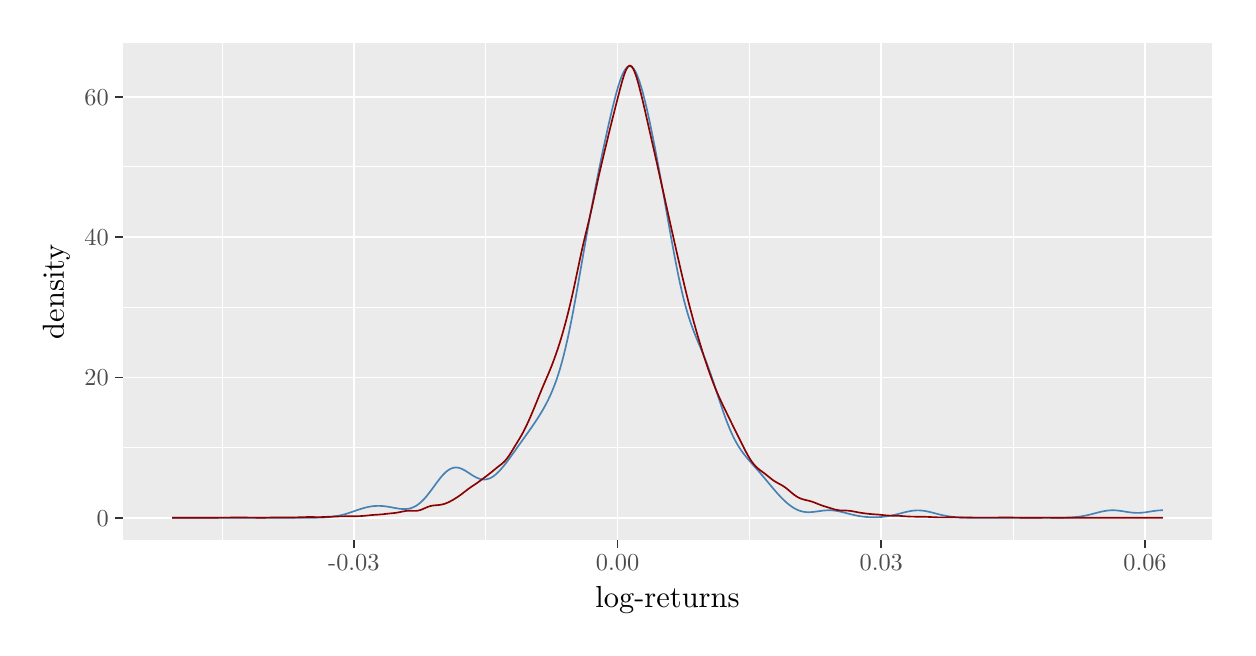
\begin{tikzpicture}[x=1pt,y=1pt]
\definecolor{fillColor}{RGB}{255,255,255}
\path[use as bounding box,fill=fillColor,fill opacity=0.00] (0,0) rectangle (433.62,216.81);
\begin{scope}
\path[clip] (  0.00,  0.00) rectangle (433.62,216.81);
\definecolor{drawColor}{RGB}{255,255,255}
\definecolor{fillColor}{RGB}{255,255,255}

\path[draw=drawColor,line width= 0.6pt,line join=round,line cap=round,fill=fillColor] (  0.00,  0.00) rectangle (433.62,216.81);
\end{scope}
\begin{scope}
\path[clip] ( 34.27, 31.53) rectangle (428.12,211.31);
\definecolor{fillColor}{gray}{0.92}

\path[fill=fillColor] ( 34.27, 31.53) rectangle (428.12,211.31);
\definecolor{drawColor}{RGB}{255,255,255}

\path[draw=drawColor,line width= 0.3pt,line join=round] ( 34.27, 65.06) --
	(428.12, 65.06);

\path[draw=drawColor,line width= 0.3pt,line join=round] ( 34.27,115.78) --
	(428.12,115.78);

\path[draw=drawColor,line width= 0.3pt,line join=round] ( 34.27,166.50) --
	(428.12,166.50);

\path[draw=drawColor,line width= 0.3pt,line join=round] ( 70.24, 31.53) --
	( 70.24,211.31);

\path[draw=drawColor,line width= 0.3pt,line join=round] (165.52, 31.53) --
	(165.52,211.31);

\path[draw=drawColor,line width= 0.3pt,line join=round] (260.81, 31.53) --
	(260.81,211.31);

\path[draw=drawColor,line width= 0.3pt,line join=round] (356.09, 31.53) --
	(356.09,211.31);

\path[draw=drawColor,line width= 0.6pt,line join=round] ( 34.27, 39.70) --
	(428.12, 39.70);

\path[draw=drawColor,line width= 0.6pt,line join=round] ( 34.27, 90.42) --
	(428.12, 90.42);

\path[draw=drawColor,line width= 0.6pt,line join=round] ( 34.27,141.14) --
	(428.12,141.14);

\path[draw=drawColor,line width= 0.6pt,line join=round] ( 34.27,191.86) --
	(428.12,191.86);

\path[draw=drawColor,line width= 0.6pt,line join=round] (117.88, 31.53) --
	(117.88,211.31);

\path[draw=drawColor,line width= 0.6pt,line join=round] (213.17, 31.53) --
	(213.17,211.31);

\path[draw=drawColor,line width= 0.6pt,line join=round] (308.45, 31.53) --
	(308.45,211.31);

\path[draw=drawColor,line width= 0.6pt,line join=round] (403.74, 31.53) --
	(403.74,211.31);
\definecolor{drawColor}{RGB}{70,130,180}

\path[draw=drawColor,line width= 0.6pt,line join=round] ( 52.17, 39.70) --
	( 52.87, 39.70) --
	( 53.57, 39.70) --
	( 54.27, 39.70) --
	( 54.97, 39.70) --
	( 55.67, 39.70) --
	( 56.37, 39.70) --
	( 57.07, 39.70) --
	( 57.78, 39.70) --
	( 58.48, 39.70) --
	( 59.18, 39.70) --
	( 59.88, 39.70) --
	( 60.58, 39.70) --
	( 61.28, 39.70) --
	( 61.98, 39.70) --
	( 62.68, 39.70) --
	( 63.38, 39.70) --
	( 64.08, 39.70) --
	( 64.78, 39.70) --
	( 65.48, 39.70) --
	( 66.18, 39.70) --
	( 66.88, 39.70) --
	( 67.59, 39.70) --
	( 68.29, 39.70) --
	( 68.99, 39.70) --
	( 69.69, 39.70) --
	( 70.39, 39.70) --
	( 71.09, 39.70) --
	( 71.79, 39.70) --
	( 72.49, 39.70) --
	( 73.19, 39.70) --
	( 73.89, 39.70) --
	( 74.59, 39.70) --
	( 75.29, 39.70) --
	( 75.99, 39.70) --
	( 76.69, 39.70) --
	( 77.39, 39.70) --
	( 78.10, 39.70) --
	( 78.80, 39.70) --
	( 79.50, 39.70) --
	( 80.20, 39.70) --
	( 80.90, 39.70) --
	( 81.60, 39.70) --
	( 82.30, 39.70) --
	( 83.00, 39.70) --
	( 83.70, 39.70) --
	( 84.40, 39.70) --
	( 85.10, 39.70) --
	( 85.80, 39.70) --
	( 86.50, 39.70) --
	( 87.20, 39.70) --
	( 87.90, 39.70) --
	( 88.61, 39.70) --
	( 89.31, 39.70) --
	( 90.01, 39.70) --
	( 90.71, 39.70) --
	( 91.41, 39.70) --
	( 92.11, 39.70) --
	( 92.81, 39.70) --
	( 93.51, 39.70) --
	( 94.21, 39.70) --
	( 94.91, 39.70) --
	( 95.61, 39.70) --
	( 96.31, 39.70) --
	( 97.01, 39.70) --
	( 97.71, 39.70) --
	( 98.42, 39.70) --
	( 99.12, 39.70) --
	( 99.82, 39.71) --
	(100.52, 39.71) --
	(101.22, 39.71) --
	(101.92, 39.71) --
	(102.62, 39.72) --
	(103.32, 39.73) --
	(104.02, 39.73) --
	(104.72, 39.75) --
	(105.42, 39.76) --
	(106.12, 39.79) --
	(106.82, 39.82) --
	(107.52, 39.85) --
	(108.22, 39.90) --
	(108.93, 39.95) --
	(109.63, 40.02) --
	(110.33, 40.11) --
	(111.03, 40.21) --
	(111.73, 40.33) --
	(112.43, 40.46) --
	(113.13, 40.62) --
	(113.83, 40.79) --
	(114.53, 40.98) --
	(115.23, 41.18) --
	(115.93, 41.40) --
	(116.63, 41.64) --
	(117.33, 41.88) --
	(118.03, 42.12) --
	(118.73, 42.36) --
	(119.44, 42.60) --
	(120.14, 42.83) --
	(120.84, 43.05) --
	(121.54, 43.26) --
	(122.24, 43.44) --
	(122.94, 43.60) --
	(123.64, 43.74) --
	(124.34, 43.85) --
	(125.04, 43.93) --
	(125.74, 43.98) --
	(126.44, 44.01) --
	(127.14, 44.01) --
	(127.84, 43.98) --
	(128.54, 43.92) --
	(129.24, 43.84) --
	(129.95, 43.75) --
	(130.65, 43.63) --
	(131.35, 43.51) --
	(132.05, 43.37) --
	(132.75, 43.24) --
	(133.45, 43.12) --
	(134.15, 43.01) --
	(134.85, 42.92) --
	(135.55, 42.87) --
	(136.25, 42.86) --
	(136.95, 42.90) --
	(137.65, 42.99) --
	(138.35, 43.15) --
	(139.05, 43.39) --
	(139.76, 43.71) --
	(140.46, 44.10) --
	(141.16, 44.59) --
	(141.86, 45.15) --
	(142.56, 45.79) --
	(143.26, 46.51) --
	(143.96, 47.30) --
	(144.66, 48.15) --
	(145.36, 49.06) --
	(146.06, 50.00) --
	(146.76, 50.96) --
	(147.46, 51.92) --
	(148.16, 52.86) --
	(148.86, 53.77) --
	(149.56, 54.63) --
	(150.27, 55.42) --
	(150.97, 56.12) --
	(151.67, 56.70) --
	(152.37, 57.18) --
	(153.07, 57.53) --
	(153.77, 57.76) --
	(154.47, 57.87) --
	(155.17, 57.86) --
	(155.87, 57.74) --
	(156.57, 57.50) --
	(157.27, 57.19) --
	(157.97, 56.81) --
	(158.67, 56.38) --
	(159.37, 55.93) --
	(160.07, 55.47) --
	(160.78, 55.02) --
	(161.48, 54.60) --
	(162.18, 54.24) --
	(162.88, 53.94) --
	(163.58, 53.71) --
	(164.28, 53.58) --
	(164.98, 53.53) --
	(165.68, 53.59) --
	(166.38, 53.75) --
	(167.08, 54.01) --
	(167.78, 54.38) --
	(168.48, 54.85) --
	(169.18, 55.41) --
	(169.88, 56.06) --
	(170.59, 56.78) --
	(171.29, 57.57) --
	(171.99, 58.41) --
	(172.69, 59.29) --
	(173.39, 60.22) --
	(174.09, 61.17) --
	(174.79, 62.14) --
	(175.49, 63.11) --
	(176.19, 64.09) --
	(176.89, 65.08) --
	(177.59, 66.06) --
	(178.29, 67.04) --
	(178.99, 68.02) --
	(179.69, 69.01) --
	(180.39, 69.99) --
	(181.10, 70.98) --
	(181.80, 71.98) --
	(182.50, 72.99) --
	(183.20, 74.02) --
	(183.90, 75.08) --
	(184.60, 76.16) --
	(185.30, 77.29) --
	(186.00, 78.46) --
	(186.70, 79.69) --
	(187.40, 80.99) --
	(188.10, 82.37) --
	(188.80, 83.85) --
	(189.50, 85.45) --
	(190.20, 87.18) --
	(190.90, 89.06) --
	(191.61, 91.13) --
	(192.31, 93.39) --
	(193.01, 95.84) --
	(193.71, 98.50) --
	(194.41,101.37) --
	(195.11,104.44) --
	(195.81,107.72) --
	(196.51,111.18) --
	(197.21,114.84) --
	(197.91,118.64) --
	(198.61,122.55) --
	(199.31,126.53) --
	(200.01,130.56) --
	(200.71,134.61) --
	(201.42,138.64) --
	(202.12,142.64) --
	(202.82,146.56) --
	(203.52,150.40) --
	(204.22,154.16) --
	(204.92,157.82) --
	(205.62,161.40) --
	(206.32,164.89) --
	(207.02,168.31) --
	(207.72,171.67) --
	(208.42,174.96) --
	(209.12,178.18) --
	(209.82,181.34) --
	(210.52,184.42) --
	(211.22,187.39) --
	(211.93,190.23) --
	(212.63,192.91) --
	(213.33,195.37) --
	(214.03,197.57) --
	(214.73,199.42) --
	(215.43,200.91) --
	(216.13,202.01) --
	(216.83,202.68) --
	(217.53,202.92) --
	(218.23,202.70) --
	(218.93,202.04) --
	(219.63,200.95) --
	(220.33,199.40) --
	(221.03,197.48) --
	(221.73,195.24) --
	(222.44,192.72) --
	(223.14,189.95) --
	(223.84,186.97) --
	(224.54,183.82) --
	(225.24,180.50) --
	(225.94,177.05) --
	(226.64,173.48) --
	(227.34,169.81) --
	(228.04,166.05) --
	(228.74,162.21) --
	(229.44,158.31) --
	(230.14,154.36) --
	(230.84,150.38) --
	(231.54,146.39) --
	(232.24,142.44) --
	(232.95,138.55) --
	(233.65,134.76) --
	(234.35,131.10) --
	(235.05,127.60) --
	(235.75,124.30) --
	(236.45,121.20) --
	(237.15,118.33) --
	(237.85,115.71) --
	(238.55,113.30) --
	(239.25,111.10) --
	(239.95,109.07) --
	(240.65,107.18) --
	(241.35,105.40) --
	(242.05,103.69) --
	(242.76,102.03) --
	(243.46,100.36) --
	(244.16, 98.65) --
	(244.86, 96.89) --
	(245.56, 95.06) --
	(246.26, 93.15) --
	(246.96, 91.17) --
	(247.66, 89.12) --
	(248.36, 87.01) --
	(249.06, 84.88) --
	(249.76, 82.74) --
	(250.46, 80.63) --
	(251.16, 78.56) --
	(251.86, 76.56) --
	(252.56, 74.65) --
	(253.27, 72.85) --
	(253.97, 71.16) --
	(254.67, 69.61) --
	(255.37, 68.18) --
	(256.07, 66.88) --
	(256.77, 65.68) --
	(257.47, 64.59) --
	(258.17, 63.58) --
	(258.87, 62.64) --
	(259.57, 61.76) --
	(260.27, 60.92) --
	(260.97, 60.11) --
	(261.67, 59.31) --
	(262.37, 58.53) --
	(263.07, 57.73) --
	(263.78, 56.94) --
	(264.48, 56.13) --
	(265.18, 55.31) --
	(265.88, 54.49) --
	(266.58, 53.65) --
	(267.28, 52.81) --
	(267.98, 51.97) --
	(268.68, 51.13) --
	(269.38, 50.30) --
	(270.08, 49.48) --
	(270.78, 48.68) --
	(271.48, 47.90) --
	(272.18, 47.16) --
	(272.88, 46.44) --
	(273.59, 45.77) --
	(274.29, 45.13) --
	(274.99, 44.55) --
	(275.69, 44.01) --
	(276.39, 43.53) --
	(277.09, 43.10) --
	(277.79, 42.73) --
	(278.49, 42.42) --
	(279.19, 42.18) --
	(279.89, 41.99) --
	(280.59, 41.85) --
	(281.29, 41.77) --
	(281.99, 41.73) --
	(282.69, 41.74) --
	(283.39, 41.78) --
	(284.10, 41.85) --
	(284.80, 41.94) --
	(285.50, 42.03) --
	(286.20, 42.13) --
	(286.90, 42.23) --
	(287.60, 42.31) --
	(288.30, 42.37) --
	(289.00, 42.41) --
	(289.70, 42.42) --
	(290.40, 42.40) --
	(291.10, 42.35) --
	(291.80, 42.27) --
	(292.50, 42.16) --
	(293.20, 42.03) --
	(293.90, 41.87) --
	(294.61, 41.71) --
	(295.31, 41.53) --
	(296.01, 41.34) --
	(296.71, 41.16) --
	(297.41, 40.98) --
	(298.11, 40.81) --
	(298.81, 40.65) --
	(299.51, 40.50) --
	(300.21, 40.37) --
	(300.91, 40.25) --
	(301.61, 40.16) --
	(302.31, 40.08) --
	(303.01, 40.01) --
	(303.71, 39.96) --
	(304.41, 39.93) --
	(305.12, 39.90) --
	(305.82, 39.90) --
	(306.52, 39.90) --
	(307.22, 39.93) --
	(307.92, 39.97) --
	(308.62, 40.02) --
	(309.32, 40.09) --
	(310.02, 40.17) --
	(310.72, 40.27) --
	(311.42, 40.39) --
	(312.12, 40.52) --
	(312.82, 40.67) --
	(313.52, 40.83) --
	(314.22, 41.00) --
	(314.93, 41.18) --
	(315.63, 41.36) --
	(316.33, 41.55) --
	(317.03, 41.73) --
	(317.73, 41.89) --
	(318.43, 42.04) --
	(319.13, 42.17) --
	(319.83, 42.27) --
	(320.53, 42.34) --
	(321.23, 42.38) --
	(321.93, 42.38) --
	(322.63, 42.36) --
	(323.33, 42.29) --
	(324.03, 42.20) --
	(324.73, 42.08) --
	(325.44, 41.93) --
	(326.14, 41.77) --
	(326.84, 41.60) --
	(327.54, 41.41) --
	(328.24, 41.23) --
	(328.94, 41.05) --
	(329.64, 40.87) --
	(330.34, 40.70) --
	(331.04, 40.55) --
	(331.74, 40.41) --
	(332.44, 40.29) --
	(333.14, 40.18) --
	(333.84, 40.09) --
	(334.54, 40.01) --
	(335.24, 39.94) --
	(335.95, 39.89) --
	(336.65, 39.84) --
	(337.35, 39.81) --
	(338.05, 39.78) --
	(338.75, 39.76) --
	(339.45, 39.75) --
	(340.15, 39.73) --
	(340.85, 39.72) --
	(341.55, 39.72) --
	(342.25, 39.71) --
	(342.95, 39.71) --
	(343.65, 39.71) --
	(344.35, 39.71) --
	(345.05, 39.70) --
	(345.76, 39.70) --
	(346.46, 39.70) --
	(347.16, 39.70) --
	(347.86, 39.70) --
	(348.56, 39.70) --
	(349.26, 39.70) --
	(349.96, 39.70) --
	(350.66, 39.70) --
	(351.36, 39.70) --
	(352.06, 39.70) --
	(352.76, 39.70) --
	(353.46, 39.70) --
	(354.16, 39.70) --
	(354.86, 39.70) --
	(355.56, 39.70) --
	(356.27, 39.70) --
	(356.97, 39.70) --
	(357.67, 39.70) --
	(358.37, 39.70) --
	(359.07, 39.70) --
	(359.77, 39.70) --
	(360.47, 39.70) --
	(361.17, 39.70) --
	(361.87, 39.70) --
	(362.57, 39.70) --
	(363.27, 39.70) --
	(363.97, 39.70) --
	(364.67, 39.70) --
	(365.37, 39.70) --
	(366.07, 39.70) --
	(366.78, 39.70) --
	(367.48, 39.70) --
	(368.18, 39.70) --
	(368.88, 39.71) --
	(369.58, 39.71) --
	(370.28, 39.71) --
	(370.98, 39.71) --
	(371.68, 39.72) --
	(372.38, 39.72) --
	(373.08, 39.73) --
	(373.78, 39.74) --
	(374.48, 39.75) --
	(375.18, 39.77) --
	(375.88, 39.80) --
	(376.58, 39.83) --
	(377.29, 39.87) --
	(377.99, 39.92) --
	(378.69, 39.98) --
	(379.39, 40.06) --
	(380.09, 40.14) --
	(380.79, 40.25) --
	(381.49, 40.36) --
	(382.19, 40.50) --
	(382.89, 40.64) --
	(383.59, 40.81) --
	(384.29, 40.98) --
	(384.99, 41.16) --
	(385.69, 41.34) --
	(386.39, 41.53) --
	(387.10, 41.71) --
	(387.80, 41.88) --
	(388.50, 42.03) --
	(389.20, 42.16) --
	(389.90, 42.27) --
	(390.60, 42.35) --
	(391.30, 42.40) --
	(392.00, 42.42) --
	(392.70, 42.41) --
	(393.40, 42.37) --
	(394.10, 42.30) --
	(394.80, 42.21) --
	(395.50, 42.11) --
	(396.20, 42.00) --
	(396.90, 41.88) --
	(397.61, 41.77) --
	(398.31, 41.67) --
	(399.01, 41.59) --
	(399.71, 41.52) --
	(400.41, 41.49) --
	(401.11, 41.48) --
	(401.81, 41.50) --
	(402.51, 41.54) --
	(403.21, 41.61) --
	(403.91, 41.69) --
	(404.61, 41.80) --
	(405.31, 41.91) --
	(406.01, 42.02) --
	(406.71, 42.13) --
	(407.41, 42.23) --
	(408.12, 42.32) --
	(408.82, 42.38) --
	(409.52, 42.41) --
	(410.22, 42.42);
\definecolor{drawColor}{RGB}{139,0,0}

\path[draw=drawColor,line width= 0.6pt,line join=round] ( 52.17, 39.73) --
	( 52.87, 39.73) --
	( 53.57, 39.73) --
	( 54.27, 39.72) --
	( 54.97, 39.72) --
	( 55.67, 39.72) --
	( 56.37, 39.72) --
	( 57.07, 39.72) --
	( 57.78, 39.72) --
	( 58.48, 39.73) --
	( 59.18, 39.73) --
	( 59.88, 39.73) --
	( 60.58, 39.73) --
	( 61.28, 39.73) --
	( 61.98, 39.72) --
	( 62.68, 39.72) --
	( 63.38, 39.71) --
	( 64.08, 39.71) --
	( 64.78, 39.71) --
	( 65.48, 39.71) --
	( 66.18, 39.71) --
	( 66.88, 39.72) --
	( 67.59, 39.73) --
	( 68.29, 39.74) --
	( 68.99, 39.75) --
	( 69.69, 39.76) --
	( 70.39, 39.77) --
	( 71.09, 39.77) --
	( 71.79, 39.78) --
	( 72.49, 39.78) --
	( 73.19, 39.78) --
	( 73.89, 39.79) --
	( 74.59, 39.80) --
	( 75.29, 39.80) --
	( 75.99, 39.81) --
	( 76.69, 39.81) --
	( 77.39, 39.80) --
	( 78.10, 39.80) --
	( 78.80, 39.79) --
	( 79.50, 39.78) --
	( 80.20, 39.78) --
	( 80.90, 39.77) --
	( 81.60, 39.76) --
	( 82.30, 39.75) --
	( 83.00, 39.74) --
	( 83.70, 39.74) --
	( 84.40, 39.73) --
	( 85.10, 39.74) --
	( 85.80, 39.74) --
	( 86.50, 39.76) --
	( 87.20, 39.77) --
	( 87.90, 39.79) --
	( 88.61, 39.81) --
	( 89.31, 39.82) --
	( 90.01, 39.82) --
	( 90.71, 39.82) --
	( 91.41, 39.82) --
	( 92.11, 39.81) --
	( 92.81, 39.80) --
	( 93.51, 39.80) --
	( 94.21, 39.80) --
	( 94.91, 39.81) --
	( 95.61, 39.82) --
	( 96.31, 39.83) --
	( 97.01, 39.85) --
	( 97.71, 39.87) --
	( 98.42, 39.90) --
	( 99.12, 39.92) --
	( 99.82, 39.94) --
	(100.52, 39.96) --
	(101.22, 39.98) --
	(101.92, 39.98) --
	(102.62, 39.98) --
	(103.32, 39.97) --
	(104.02, 39.95) --
	(104.72, 39.94) --
	(105.42, 39.95) --
	(106.12, 39.96) --
	(106.82, 39.98) --
	(107.52, 40.02) --
	(108.22, 40.06) --
	(108.93, 40.09) --
	(109.63, 40.12) --
	(110.33, 40.15) --
	(111.03, 40.17) --
	(111.73, 40.18) --
	(112.43, 40.20) --
	(113.13, 40.21) --
	(113.83, 40.22) --
	(114.53, 40.24) --
	(115.23, 40.25) --
	(115.93, 40.26) --
	(116.63, 40.26) --
	(117.33, 40.26) --
	(118.03, 40.26) --
	(118.73, 40.27) --
	(119.44, 40.29) --
	(120.14, 40.31) --
	(120.84, 40.36) --
	(121.54, 40.41) --
	(122.24, 40.48) --
	(122.94, 40.55) --
	(123.64, 40.62) --
	(124.34, 40.69) --
	(125.04, 40.75) --
	(125.74, 40.79) --
	(126.44, 40.83) --
	(127.14, 40.88) --
	(127.84, 40.94) --
	(128.54, 41.01) --
	(129.24, 41.09) --
	(129.95, 41.17) --
	(130.65, 41.25) --
	(131.35, 41.32) --
	(132.05, 41.39) --
	(132.75, 41.46) --
	(133.45, 41.56) --
	(134.15, 41.69) --
	(134.85, 41.83) --
	(135.55, 41.98) --
	(136.25, 42.11) --
	(136.95, 42.20) --
	(137.65, 42.24) --
	(138.35, 42.24) --
	(139.05, 42.21) --
	(139.76, 42.19) --
	(140.46, 42.22) --
	(141.16, 42.32) --
	(141.86, 42.50) --
	(142.56, 42.76) --
	(143.26, 43.07) --
	(143.96, 43.38) --
	(144.66, 43.67) --
	(145.36, 43.91) --
	(146.06, 44.07) --
	(146.76, 44.17) --
	(147.46, 44.24) --
	(148.16, 44.29) --
	(148.86, 44.37) --
	(149.56, 44.48) --
	(150.27, 44.65) --
	(150.97, 44.87) --
	(151.67, 45.15) --
	(152.37, 45.48) --
	(153.07, 45.85) --
	(153.77, 46.24) --
	(154.47, 46.67) --
	(155.17, 47.11) --
	(155.87, 47.59) --
	(156.57, 48.09) --
	(157.27, 48.62) --
	(157.97, 49.16) --
	(158.67, 49.71) --
	(159.37, 50.23) --
	(160.07, 50.73) --
	(160.78, 51.20) --
	(161.48, 51.67) --
	(162.18, 52.14) --
	(162.88, 52.64) --
	(163.58, 53.15) --
	(164.28, 53.67) --
	(164.98, 54.20) --
	(165.68, 54.72) --
	(166.38, 55.25) --
	(167.08, 55.80) --
	(167.78, 56.36) --
	(168.48, 56.94) --
	(169.18, 57.51) --
	(169.88, 58.07) --
	(170.59, 58.61) --
	(171.29, 59.17) --
	(171.99, 59.78) --
	(172.69, 60.51) --
	(173.39, 61.38) --
	(174.09, 62.39) --
	(174.79, 63.50) --
	(175.49, 64.65) --
	(176.19, 65.80) --
	(176.89, 66.95) --
	(177.59, 68.09) --
	(178.29, 69.28) --
	(178.99, 70.55) --
	(179.69, 71.90) --
	(180.39, 73.36) --
	(181.10, 74.89) --
	(181.80, 76.49) --
	(182.50, 78.14) --
	(183.20, 79.83) --
	(183.90, 81.54) --
	(184.60, 83.28) --
	(185.30, 85.00) --
	(186.00, 86.69) --
	(186.70, 88.35) --
	(187.40, 89.97) --
	(188.10, 91.60) --
	(188.80, 93.28) --
	(189.50, 95.05) --
	(190.20, 96.90) --
	(190.90, 98.86) --
	(191.61,100.93) --
	(192.31,103.11) --
	(193.01,105.41) --
	(193.71,107.85) --
	(194.41,110.42) --
	(195.11,113.12) --
	(195.81,115.95) --
	(196.51,118.93) --
	(197.21,122.05) --
	(197.91,125.30) --
	(198.61,128.64) --
	(199.31,132.00) --
	(200.01,135.28) --
	(200.71,138.41) --
	(201.42,141.40) --
	(202.12,144.29) --
	(202.82,147.18) --
	(203.52,150.19) --
	(204.22,153.33) --
	(204.92,156.57) --
	(205.62,159.82) --
	(206.32,163.01) --
	(207.02,166.07) --
	(207.72,169.04) --
	(208.42,171.96) --
	(209.12,174.86) --
	(209.82,177.78) --
	(210.52,180.68) --
	(211.22,183.53) --
	(211.93,186.33) --
	(212.63,189.09) --
	(213.33,191.82) --
	(214.03,194.52) --
	(214.73,197.11) --
	(215.43,199.46) --
	(216.13,201.37) --
	(216.83,202.65) --
	(217.53,203.14) --
	(218.23,202.82) --
	(218.93,201.74) --
	(219.63,200.03) --
	(220.33,197.82) --
	(221.03,195.27) --
	(221.73,192.47) --
	(222.44,189.53) --
	(223.14,186.50) --
	(223.84,183.42) --
	(224.54,180.33) --
	(225.24,177.23) --
	(225.94,174.14) --
	(226.64,171.04) --
	(227.34,167.92) --
	(228.04,164.80) --
	(228.74,161.65) --
	(229.44,158.50) --
	(230.14,155.34) --
	(230.84,152.18) --
	(231.54,149.02) --
	(232.24,145.85) --
	(232.95,142.70) --
	(233.65,139.57) --
	(234.35,136.47) --
	(235.05,133.39) --
	(235.75,130.34) --
	(236.45,127.32) --
	(237.15,124.35) --
	(237.85,121.44) --
	(238.55,118.62) --
	(239.25,115.89) --
	(239.95,113.24) --
	(240.65,110.66) --
	(241.35,108.15) --
	(242.05,105.69) --
	(242.76,103.29) --
	(243.46,100.96) --
	(244.16, 98.71) --
	(244.86, 96.54) --
	(245.56, 94.44) --
	(246.26, 92.43) --
	(246.96, 90.48) --
	(247.66, 88.61) --
	(248.36, 86.82) --
	(249.06, 85.13) --
	(249.76, 83.52) --
	(250.46, 81.99) --
	(251.16, 80.51) --
	(251.86, 79.06) --
	(252.56, 77.62) --
	(253.27, 76.18) --
	(253.97, 74.73) --
	(254.67, 73.30) --
	(255.37, 71.89) --
	(256.07, 70.49) --
	(256.77, 69.09) --
	(257.47, 67.68) --
	(258.17, 66.26) --
	(258.87, 64.86) --
	(259.57, 63.49) --
	(260.27, 62.21) --
	(260.97, 61.03) --
	(261.67, 59.98) --
	(262.37, 59.07) --
	(263.07, 58.28) --
	(263.78, 57.62) --
	(264.48, 57.04) --
	(265.18, 56.52) --
	(265.88, 56.01) --
	(266.58, 55.48) --
	(267.28, 54.92) --
	(267.98, 54.36) --
	(268.68, 53.80) --
	(269.38, 53.27) --
	(270.08, 52.81) --
	(270.78, 52.40) --
	(271.48, 52.02) --
	(272.18, 51.65) --
	(272.88, 51.24) --
	(273.59, 50.78) --
	(274.29, 50.25) --
	(274.99, 49.66) --
	(275.69, 49.06) --
	(276.39, 48.47) --
	(277.09, 47.92) --
	(277.79, 47.44) --
	(278.49, 47.03) --
	(279.19, 46.71) --
	(279.89, 46.45) --
	(280.59, 46.26) --
	(281.29, 46.09) --
	(281.99, 45.93) --
	(282.69, 45.75) --
	(283.39, 45.54) --
	(284.10, 45.29) --
	(284.80, 45.01) --
	(285.50, 44.73) --
	(286.20, 44.46) --
	(286.90, 44.20) --
	(287.60, 43.96) --
	(288.30, 43.74) --
	(289.00, 43.53) --
	(289.70, 43.31) --
	(290.40, 43.09) --
	(291.10, 42.87) --
	(291.80, 42.68) --
	(292.50, 42.52) --
	(293.20, 42.42) --
	(293.90, 42.36) --
	(294.61, 42.34) --
	(295.31, 42.33) --
	(296.01, 42.31) --
	(296.71, 42.26) --
	(297.41, 42.17) --
	(298.11, 42.06) --
	(298.81, 41.92) --
	(299.51, 41.78) --
	(300.21, 41.65) --
	(300.91, 41.53) --
	(301.61, 41.43) --
	(302.31, 41.33) --
	(303.01, 41.24) --
	(303.71, 41.16) --
	(304.41, 41.08) --
	(305.12, 41.02) --
	(305.82, 40.97) --
	(306.52, 40.93) --
	(307.22, 40.88) --
	(307.92, 40.82) --
	(308.62, 40.74) --
	(309.32, 40.66) --
	(310.02, 40.59) --
	(310.72, 40.53) --
	(311.42, 40.49) --
	(312.12, 40.47) --
	(312.82, 40.47) --
	(313.52, 40.46) --
	(314.22, 40.45) --
	(314.93, 40.41) --
	(315.63, 40.36) --
	(316.33, 40.30) --
	(317.03, 40.25) --
	(317.73, 40.20) --
	(318.43, 40.16) --
	(319.13, 40.14) --
	(319.83, 40.12) --
	(320.53, 40.11) --
	(321.23, 40.10) --
	(321.93, 40.09) --
	(322.63, 40.09) --
	(323.33, 40.08) --
	(324.03, 40.06) --
	(324.73, 40.05) --
	(325.44, 40.02) --
	(326.14, 39.99) --
	(326.84, 39.95) --
	(327.54, 39.92) --
	(328.24, 39.89) --
	(328.94, 39.86) --
	(329.64, 39.85) --
	(330.34, 39.85) --
	(331.04, 39.86) --
	(331.74, 39.87) --
	(332.44, 39.88) --
	(333.14, 39.89) --
	(333.84, 39.89) --
	(334.54, 39.89) --
	(335.24, 39.87) --
	(335.95, 39.86) --
	(336.65, 39.84) --
	(337.35, 39.83) --
	(338.05, 39.82) --
	(338.75, 39.82) --
	(339.45, 39.81) --
	(340.15, 39.80) --
	(340.85, 39.79) --
	(341.55, 39.78) --
	(342.25, 39.77) --
	(342.95, 39.76) --
	(343.65, 39.76) --
	(344.35, 39.75) --
	(345.05, 39.75) --
	(345.76, 39.75) --
	(346.46, 39.75) --
	(347.16, 39.76) --
	(347.86, 39.76) --
	(348.56, 39.77) --
	(349.26, 39.77) --
	(349.96, 39.78) --
	(350.66, 39.78) --
	(351.36, 39.79) --
	(352.06, 39.79) --
	(352.76, 39.80) --
	(353.46, 39.80) --
	(354.16, 39.80) --
	(354.86, 39.80) --
	(355.56, 39.79) --
	(356.27, 39.78) --
	(356.97, 39.77) --
	(357.67, 39.76) --
	(358.37, 39.75) --
	(359.07, 39.74) --
	(359.77, 39.73) --
	(360.47, 39.73) --
	(361.17, 39.72) --
	(361.87, 39.71) --
	(362.57, 39.71) --
	(363.27, 39.71) --
	(363.97, 39.72) --
	(364.67, 39.72) --
	(365.37, 39.73) --
	(366.07, 39.74) --
	(366.78, 39.75) --
	(367.48, 39.76) --
	(368.18, 39.76) --
	(368.88, 39.76) --
	(369.58, 39.75) --
	(370.28, 39.74) --
	(370.98, 39.73) --
	(371.68, 39.72) --
	(372.38, 39.72) --
	(373.08, 39.71) --
	(373.78, 39.71) --
	(374.48, 39.70) --
	(375.18, 39.70) --
	(375.88, 39.70) --
	(376.58, 39.70) --
	(377.29, 39.70) --
	(377.99, 39.70) --
	(378.69, 39.70) --
	(379.39, 39.70) --
	(380.09, 39.70) --
	(380.79, 39.70) --
	(381.49, 39.70) --
	(382.19, 39.70) --
	(382.89, 39.70) --
	(383.59, 39.70) --
	(384.29, 39.70) --
	(384.99, 39.70) --
	(385.69, 39.70) --
	(386.39, 39.70) --
	(387.10, 39.70) --
	(387.80, 39.70) --
	(388.50, 39.70) --
	(389.20, 39.70) --
	(389.90, 39.70) --
	(390.60, 39.70) --
	(391.30, 39.70) --
	(392.00, 39.70) --
	(392.70, 39.70) --
	(393.40, 39.70) --
	(394.10, 39.70) --
	(394.80, 39.70) --
	(395.50, 39.70) --
	(396.20, 39.70) --
	(396.90, 39.70) --
	(397.61, 39.70) --
	(398.31, 39.70) --
	(399.01, 39.70) --
	(399.71, 39.70) --
	(400.41, 39.70) --
	(401.11, 39.70) --
	(401.81, 39.70) --
	(402.51, 39.70) --
	(403.21, 39.70) --
	(403.91, 39.70) --
	(404.61, 39.70) --
	(405.31, 39.70) --
	(406.01, 39.70) --
	(406.71, 39.70) --
	(407.41, 39.70) --
	(408.12, 39.70) --
	(408.82, 39.70) --
	(409.52, 39.70) --
	(410.22, 39.70);
\end{scope}
\begin{scope}
\path[clip] (  0.00,  0.00) rectangle (433.62,216.81);
\definecolor{drawColor}{gray}{0.30}

\node[text=drawColor,anchor=base east,inner sep=0pt, outer sep=0pt, scale=  0.88] at ( 29.32, 36.67) {0};

\node[text=drawColor,anchor=base east,inner sep=0pt, outer sep=0pt, scale=  0.88] at ( 29.32, 87.39) {20};

\node[text=drawColor,anchor=base east,inner sep=0pt, outer sep=0pt, scale=  0.88] at ( 29.32,138.11) {40};

\node[text=drawColor,anchor=base east,inner sep=0pt, outer sep=0pt, scale=  0.88] at ( 29.32,188.83) {60};
\end{scope}
\begin{scope}
\path[clip] (  0.00,  0.00) rectangle (433.62,216.81);
\definecolor{drawColor}{gray}{0.20}

\path[draw=drawColor,line width= 0.6pt,line join=round] ( 31.52, 39.70) --
	( 34.27, 39.70);

\path[draw=drawColor,line width= 0.6pt,line join=round] ( 31.52, 90.42) --
	( 34.27, 90.42);

\path[draw=drawColor,line width= 0.6pt,line join=round] ( 31.52,141.14) --
	( 34.27,141.14);

\path[draw=drawColor,line width= 0.6pt,line join=round] ( 31.52,191.86) --
	( 34.27,191.86);
\end{scope}
\begin{scope}
\path[clip] (  0.00,  0.00) rectangle (433.62,216.81);
\definecolor{drawColor}{gray}{0.20}

\path[draw=drawColor,line width= 0.6pt,line join=round] (117.88, 28.78) --
	(117.88, 31.53);

\path[draw=drawColor,line width= 0.6pt,line join=round] (213.17, 28.78) --
	(213.17, 31.53);

\path[draw=drawColor,line width= 0.6pt,line join=round] (308.45, 28.78) --
	(308.45, 31.53);

\path[draw=drawColor,line width= 0.6pt,line join=round] (403.74, 28.78) --
	(403.74, 31.53);
\end{scope}
\begin{scope}
\path[clip] (  0.00,  0.00) rectangle (433.62,216.81);
\definecolor{drawColor}{gray}{0.30}

\node[text=drawColor,anchor=base,inner sep=0pt, outer sep=0pt, scale=  0.88] at (117.88, 20.52) {-0.03};

\node[text=drawColor,anchor=base,inner sep=0pt, outer sep=0pt, scale=  0.88] at (213.17, 20.52) {0.00};

\node[text=drawColor,anchor=base,inner sep=0pt, outer sep=0pt, scale=  0.88] at (308.45, 20.52) {0.03};

\node[text=drawColor,anchor=base,inner sep=0pt, outer sep=0pt, scale=  0.88] at (403.74, 20.52) {0.06};
\end{scope}
\begin{scope}
\path[clip] (  0.00,  0.00) rectangle (433.62,216.81);
\definecolor{drawColor}{RGB}{0,0,0}

\node[text=drawColor,anchor=base,inner sep=0pt, outer sep=0pt, scale=  1.10] at (231.19,  7.44) {log-returns};
\end{scope}
\begin{scope}
\path[clip] (  0.00,  0.00) rectangle (433.62,216.81);
\definecolor{drawColor}{RGB}{0,0,0}

\node[text=drawColor,rotate= 90.00,anchor=base,inner sep=0pt, outer sep=0pt, scale=  1.10] at ( 13.08,121.42) {density};
\end{scope}
\end{tikzpicture}

  \caption{Historical and HSV related Apple stock Log-returns distribution in the risk-averse world}
  \floatfoot{The above blue density curve is constructed over the historical data of the Apple share of stock price evolution from 18th May 2017 to 18th May 2018. while the red curve is constructed from time-series genereated by the function \textit{hsv\_ts} taking the risk-averse parameters \ref{eq:methodology:arg:heston:riskaverse} as arguments.
  }
  \label{p:methodology:density:aapl:heston:riskaverse}
\end{figure}

Consequently, for the purpose of that master thesis, the set \ref{eq:methodology:arg:heston:riskaverse} is the one that will be used together with the function \textit{hsv\_ts()} whenever performing the computation of time series using the HSV model within the real world constraints.



%%%%%%%%%%%%%%%%%%%%%%%%%%%%%%%%%%%%%%%%%%%%%%%%%%%%%%%%%%%%%%%%%%%%%%%%%%%%%%%%
% SEC: DELTA HEDGING
%%%%%%%%%%%%%%%%%%%%%%%%%%%%%%%%%%%%%%%%%%%%%%%%%%%%%%%%%%%%%%%%%%%%%%%%%%%%%%%%
\section{Delta hedging}
\label{sec:methodology:delta}

In order to measure the hedging performance of the MJD and HSV models, I will (i) compute the prices of some options and then virtually sell them at that price, (ii)  construct the delta-neutral portfolio at time zero and thereafter continuously rebalance it, in accordance with the underlying asset price evolutions and (iii) measure the overall cost of the hedge as a performance indicator.




%%%%%%%%%%%%%%%%%%%%%%%%%%%%%%%%%%%%%%%%%%%%%%%%%%%%%%%%%%%%%%%%%%%%%%%%%%%%%%%%
% SUB: Determination of the option price
%%%%%%%%%%%%%%%%%%%%%%%%%%%%%%%%%%%%%%%%%%%%%%%%%%%%%%%%%%%%%%%%%%%%%%%%%%%%%%%%
\subsection{Determination of the option price}
\label{sec:methodology:determination}

The computation of the option price at time zero will depend on the underlying model to be hedged.
Indeed, the function \textit{mjd\_call} will be used to price options for which the underlying asset price evolution is driven by the MDJ model, whereas \textit{mjd\_call} will be used for HSV processes.

As explain as an introduction, I will virtually sell the options I price.
Therefore, as the writer of the options, I will raise \$ $X(0) = C_K^{m \oplus h} (0)$.
That cash will directly be put into a money market account to make it grow at a constant riskless rate all along the duration of the hedging process, namely, during the whole life of the option.

The T-bills will serve as riskless rate. According to the available data on \url{https://www.treasury.gov/}, quotes of these are given by \cref{tab:methodology:Tbill}.

\begin{table}[ht]
\centering
\begin{tabular}{cccc}
  \hline
  \multicolumn{4}{c}{T-bills} \\
  \hline
  4 weeks & 13 weeks & 26 weeks & 52 weeks \\
  1.66\% & 1.90\% & 2.09\% & 2.30\% \\
  \hline
\end{tabular}
\caption{Treasury bill quotes on 18 May 2018} 
\label{tab:methodology:Tbill}
\end{table}

The rates of \cref{tab:methodology:Tbill} are annual-base, consequently to get their countinuously compounded counterpart, EQUATION X can be used to give those given by \cref{tab:methodology:Tbill:compound}.


\begin{table}[ht]
\centering
\begin{tabular}{cccc}
  \hline
  \multicolumn{4}{c}{T-bills} \\
  \hline
  4 weeks & 13 weeks & 26 weeks & 52 weeks \\
  1.659\% & 1.896\% & 2.068\% & 2.274\% \\
  \hline
\end{tabular}
\caption{Treasury bill quotes on 18 May 2018} 
\label{tab:methodology:Tbill:compound}
\end{table}

Thereafter by applying the bootstrap method along with linear interpolation, one can find the maturity-wise related riskless rates of the Apple call option used for the current analysis. Those rates are given by \cref{tab:methodology:tbill:maturity}.

\begin{table}[ht]
\centering
\begin{tabular}{l|ccccccc}

  \hline
Maturity(in days) & 63   & 91   & 126  & 154    & 182  & 245    & 399 \\ 
Riskless rate     &  1.817\% & 1.896\% & 1.962\% & 2.015\%  & 2.068\%  & 2.139\%   & 2.311\% \\
   \hline
\end{tabular}
\caption{Maturities explored during the hedging performance measurement} 
\label{tab:methodology:tbill:maturity}
\end{table}




%%%%%%%%%%%%%%%%%%%%%%%%%%%%%%%%%%%%%%%%%%%%%%%%%%%%%%%%%%%%%%%%%%%%%%%%%%%%%%%%
% SUB: Determination of the option price
%%%%%%%%%%%%%%%%%%%%%%%%%%%%%%%%%%%%%%%%%%%%%%%%%%%%%%%%%%%%%%%%%%%%%%%%%%%%%%%%
\subsection{Construction of the delta-neutral portfolio}
\label{sec:methodology:construction}

At time zero, the built of the delta-neutral portfolio is achieved by the purchase of $\Delta(0)$ share of stock multiplying by the number of assets involving in the derivative product.
Simply put, if one wants to construct such a portfolio to cover against the possible losses incurred by the selling of a call option on one hundred shares, the number of underlying to buy at that time would be of $\Delta(t) \times 100$.
For the sake of clarity, in the analysis I will perform, it is implicit that any European call option involves the purchase of only one underlying at maturity, though.
Consequently, at time zero, the cost of such a portfolio is given by \cref{methodology:porfolio:cost:0}.

\begin{align}
p(t_0) = \Delta^{m \oplus h}(t_0) S(t_0) \label{methodology:porfolio:cost:0}
\end{align}
Where the superscripts m (Merton) and h (Heston) respectively stand for the computation of MJD and HSV delta.

The objective of that portfolio is to accurately replicate the reverse position taken in a derivative, i.e., to reproduce a position in a long European call in the case that matters for that analysis.
To be efficient in that role, it must be frequently rebalanced.

Accordingly, in order to do so, I will observe the underlying's time-series at every period of time $\delta t = 1 days$ and compute the updated value of $\Delta(t)$  at each of those observational timesteps.
Therefore, the requisite expenses aimed to keep the portfolio delta-neutral will evolve over time, as shown here below by \cref{methodology:porfolio:cost:i}.

\begin{align}
p(t_i) & = \Delta^{m \oplus h}(t_i - t_{i - 1}) S(t_i) 
,\forall i \in \mathbb{Z} : i \in \left \{1, T \right \}\label{methodology:porfolio:cost:i}
\end{align}

The aforementioned time-series that will be daily scrutinized are obviously hypothetical. They will be generated by the functions \textit{mjd\_ts} and \textit{hsv\_ts} for which the risk-averse parameters will be passed in.





%%%%%%%%%%%%%%%%%%%%%%%%%%%%%%%%%%%%%%%%%%%%%%%%%%%%%%%%%%%%%%%%%%%%%%%%%%%%%%%%
% SUB: Computation of the delta
%%%%%%%%%%%%%%%%%%%%%%%%%%%%%%%%%%%%%%%%%%%%%%%%%%%%%%%%%%%%%%%%%%%%%%%%%%%%%%%%
\subsection{Computation of the delta}
\label{sec:methodology:computation:delta}

By definition, the delta is the first derivative of the option's pricing function with respect to the stock price. It consequently, represents the instantaneous rate of change in the option value as the price of its underlying evolves, such so illustrated by \cref{eq:bsm:call}.

Although \citet{bs} gives to delta the value $\N{\dsub{+}}$, with $d_{+}$ explained by \cref{eq:dpm}, latter can only be used within the framework developed by \citet{bs}, that is, if the underlying is driven by a geometric Brownian motion, the volatility is deterministic, or if no jump occurs.
Accordingly, the solution to compute the delta provided by \citet{bs} cannot be used for such the MJD and HSV models.

By following the definition of delta and because the pricing function of a European call option, for which the underlying asset price evolution is driven by either the MDJ or HSV models, is given by \cref{eq:other:call:heston}, then, the \cref{eq:methodology:delta:mh} gives the solution to compute the delta for such models.

\begin{align}
&\Delta^{m \oplus h}\left(t, S(t)\right)  =
  P_1^{m \oplus h} + 
  S(t) \frac{\partial P_1^{m \oplus h}}{\partial S(t)} - 
  e^{-r(T-t)} K \frac{\partial P_2^{m \oplus h}}{\partial S(t)}
\label{eq:methodology:delta:mh}
\intertext{where}
&\frac{\partial P_1^{m \oplus h}}{\partial S(t)} = 
  \frac{1}{\pi}
  \int_0^{\infty} Re \left[
    \frac{i \phi \exp\left( -i\phi\ln K \right)} {- \phi^2 \psi^{m \oplus h}(-i)^2}  \right. \notag\\
    &\left.
    \mspace{150mu} \times \left(
      \frac{\partial\psi^{m \oplus h}(\phi - i)}{\partial S(t)} \psi^{m \oplus h}(-i) -
      \psi^{m \oplus h}(\phi-i) \frac{\partial\psi^{m \oplus h}(-i)}{\partial S(t)}
    \right)
  \right] d\phi \label{eq:methodology:delta:p1} \\
\intertext{and}
&\frac{\partial P_2^{m \oplus h}}{\partial S(t)} =
\frac{1}{\pi}
  \int_0^{\infty} Re \left(
    \frac{\exp\left( -i \phi \ln K \right)}{i \phi}
    \frac{\partial \psi^{m \oplus h}(\phi)}{\partial S(t)}
  \right)d\phi \label{eq:methodology:delta:p2}
\end{align}

Hence, the \cref{eq:methodology:delta:mh} is the one to solve for both MJD and HSV models to find them the delta at time t.
\Cref{eq:methodology:delta:p1,eq:methodology:delta:p2} can be solved by finding the first derivatives of the characteristic functions of MJD and HSV processes with respect to the stock price. 
By the way, it turns out that both of these have the same form.
\Cref{eq:methodology:psi:derivative:1} gives the solution of these derivatives, the term $\psi^{m \oplus h}(x)$ have to be replaced by the appropriate characteristic function.

\begin{align}
  \frac{\partial\psi^{m \oplus h}(x)}{\partial S(t)} =
    \psi^{m \oplus h}{(x)} \frac{ix}{S(t)} 
    \label{eq:methodology:psi:derivative:1}
\end{align}

By replacing all the derivative operations inside \cref{eq:methodology:delta:p1,eq:methodology:delta:p2} by \cref{eq:methodology:psi:derivative:1}, one finds the solved version given by \cref{eq:methodology:delta:p1:solved,eq:methodology:delta:p2:solved}. 

\begin{align}
&\frac{\partial P_1^{m \oplus h}}{\partial S(t)} = 
  \frac{1}{\pi}
  \int_0^{\infty} Re \left[
    \frac{\exp\left( -i \phi \ln K \right) \psi^{m \oplus h}(\phi -i)}
      {S(t)\psi^{m \oplus h}(-i)}
  \right] d\phi \label{eq:methodology:delta:p1:solved} \\
% \intertext{and}
&\frac{\partial P_2^{m \oplus h}}{\partial S(t)} =
\frac{1}{\pi}
  \int_0^{\infty} Re \left[
    \frac{\exp\left( -i \phi \ln K \right) \psi^{m \oplus h}(\phi)}
      {S(t)}
  \right]d\phi \label{eq:methodology:delta:p2:solved}
\end{align}

Consequently, in the extent that the term $\psi^{m \oplus h}(\phi)$ is replaced by the appropriate characteristic function, substituting \cref{eq:methodology:delta:p2:solved,eq:methodology:delta:p2:solved} into \ref{eq:methodology:delta:mh} gives \ref{eq:methodology:delta:full} that allows the computation of the delta of an option for which the underlying asset is driven by either a MJD or HSV process.


\begin{align}
  \Delta^{m \oplus h}\left(t, S(t)\right)  =
  P_1^{m \oplus h} + 
  \frac{S(t)}{\pi}
    \int_0^{\infty} Re \left[
    \frac{\exp\left( -i \phi \ln K \right) \psi^{m \oplus h}(\phi -i)}
      {S(t)\psi^{m \oplus h}(-i)}
  \right] \notag\\
    \mspace{150mu}
  - \frac{e^{-r(T-t)} K}{\pi}
    \int_0^{\infty} Re \left[
    \frac{\exp\left( -i \phi \ln K \right) \psi^{m \oplus h}(\phi)}
      {S(t)}
  \right]
\label{eq:methodology:delta:full}
\end{align}

In that respect, the R functions \textit{mjd\_delta} and \textit{hsv\_delta}, respectively compute the MJD and HSV related deltas at time $t$ by taking the risk-neutral parameters.




%%%%%%%%%%%%%%%%%%%%%%%%%%%%%%%%%%%%%%%%%%%%%%%%%%%%%%%%%%%%%%%%%%%%%%%%%%%%%%%%
% SUB: Measuring the hedging performation
%%%%%%%%%%%%%%%%%%%%%%%%%%%%%%%%%%%%%%%%%%%%%%%%%%%%%%%%%%%%%%%%%%%%%%%%%%%%%%%%
\subsection{Measuring the hedging performation}
\label{sec:methodology:measuring}

Finally, to analyze how much the hedging works, one method is to measure its overall cost.
To do so, the really first thing is to value at maturity all the buying and selling operations carried out in order to keep delta-neutral the previously constructed portfolio and add them together.

\begin{align}
  p_{tot} = \sum_{i = 0}^T p(t_i) e^{T-t_i} ,
  \forall i \in \mathbb{Z} : i \in \left \{1, T \right \}
  \label{methodology:porfolio:cost:tot}
\end{align}

On the other hand, at maturity, the amount of money $X(0)$ received when entering into the contract at time zero will have continuously grown up at the constant riskless rate $r$, as described by \cref{eq:methodology:xt}.

\begin{align}
  X(T) = X(0) * e^{rT} \label{eq:methodology:xt}
\end{align}

Incidentally, if the option is in-the-market at  maturity date, it first implies that it will be exercised, so increasing the wealth of the short position in the derivative by $K$, and then that $\Delta(T) = 1$, meaning that the writer of the option has exactly one share of stock in his / her portfolio to honour the transaction.
Otherwise, the option is out-of-the-market, inducing that no transaction occurs and that $\Delta(T) = 0$.
Consequently, at maturity, someone with a short position in the derivative, i.e., the one tempting to be replicated in the current analysis, will receive a positive cash inflow of $X(T) + \Delta(T) K$.

Hence, if the hedge works well, the relation exhibited by \ref{eq:methodology:hedge:neutral} should be respected.

\begin{align}
 \sum_{i = 0}^{n = T} P(i) \cong X(T) + \Delta(T) * k \label{eq:methodology:hedge:neutral}
\end{align}

Because the position could vary, we have to adapt the relation above (REF) in order to remove all unit from the comparison.
According to hull, a measure of performance of the hedge could be to take the ratio of the standard deviation of the cost to hedge to the option price. In that case, the measure could be comparated among themselve even if the position taken into the underlying difer.

\begin{align}
  \frac{sd(hedge)}{C_0 e ^{r T}}
  \label{bsm:delta:hedge:perf}
\end{align}
where hedge is a vector containing $n$ sample generated, and $C_0$ is the price of the call option at time zero value up to maturity.




















% \SweaveInput{analysis.Rnw}
% \SweaveInput{appendix}









\bibliography{bibl}
\bibliographystyle{plainnat}
\end{document}
